\documentclass[a4paper, 12pt]{article} % La fuente debe ser de 12pt
\usepackage[utf8]{inputenc}
\usepackage[T1]{fontenc}
\usepackage{hyperref}
\usepackage[left=3cm, right=3cm, top=3.5cm, bottom=3.5cm]{geometry} % Márgenes recomendados
\usepackage{times} % La fuente debe ser Times New Romans
\usepackage[english]{babel}
\usepackage[english]{translator}
\usepackage[style=ieee, backend=biber]{biblatex} % Bibliografía en formato IEEE
\usepackage{sectsty}
\usepackage{cover-page}
\usepackage{amsmath}
\usepackage{float}
\usepackage{minted}
\usepackage[onelanguage]{algorithm2e} %for psuedo code
\usepackage{booktabs}
\usepackage{threeparttable}
\usepackage{rotating}
\usepackage{longtable}
\usepackage{multirow}
\usepackage{multicol}
\usepackage{tablefootnote}
\usepackage{csquotes}
\usepackage{graphicx}
\usepackage{subfig}
\usepackage{cprotect}
\usepackage{subfigure}
\usepackage{pgfplots}


\usepackage[acronym]{glossaries}
\makeglossaries
% \newacronym{nn}{NN}{Neural Network}
% \newacronym{rnn}{RNN}{Recurrent Neural Network}
% \newacronym{rnns}{RNNs}{Recurrent Neural Networks}
% \newacronym{srnn}{SRNN}{Simple Recurrent Neural Network}
% \newacronym{ar}{AR}{Autoregressive}
% \newacronym{lstm}{LSTM}{Long-Short Term Memory}

% \newacronym{pss}{PSS}{Product Service System}

% \newacronym{sql}{SQL}{Structured Query Language}


% \newacronym{ai}{AI}{Artificial Intelligence}
% \newacronym{ml}{ML}{Machine Learning}
% \newacronym{dl}{DL}{Deep Learning}
% \newacronym{nlp}{NLP}{Natural Language Processing}
% \newacronym{svm}{SVM}{Support Vector Machine}


% \newacronym{xor}{XOR}{Exclusive Or}
% \newacronym{ols}{OLS}{Ordinary Least Square}


% \newacronym{csv}{CSV}{Comma-Separated Values}
% \newacronym{df}{DF}{DataFrame}


% \newacronym{relu}{ReLU}{Rectified Linear Unit}

% \newacronym{mae}{MAE}{Mean Absolute Error}
% \newacronym{mse}{MSE}{Mean Squared Error}
% \newacronym{rmse}{RMSE}{Root Mean Squared Error}
% \newacronym{msle}{MSLE}{Mean Squared Logarithmic Error}
% \newacronym{rmsle}{RMSLE}{Root Mean Squared Logarithmic Error}
% \newacronym{mape}{MAPE}{Mean Absolute Percentage Error}
% \newacronym{mpe}{MPE}{Mean Percentage Error}


% \newacronym{lr}{LR}{Learning Rate}
% \newacronym{sgd}{SGD}{Stochastic gradient descent}
% \newacronym{rmsprop}{RMSProp}{Root Mean Square Propagation}
% \newacronym{hs}{HS}{Hidden State}

% \newacronym{co2}{CO$_2$}{Carbon dioxide}

\newacronym{nn}{NN}{Red neuronal}
\newacronym{rnn}{RNN}{Red neuronal recurrente}
\newacronym{srnn}{SRNN}{Red neuronal recurrente simple}
\newacronym{ar}{AR}{Autoregressivo}
\newacronym{lstm}{LSTM}{\textit{Long-Short Term Memory}}

\newacronym{pss}{PSS}{\textit{Product Service System}}

\newacronym{sql}{SQL}{\textit{Structured Query Language}}


\newacronym{ai}{IA}{Inteligencia Artificial}
\newacronym{ml}{ML}{\textit{Machine Learning}}
\newacronym{dl}{DL}{Aprendizaje profundo}
\newacronym{nlp}{NLP}{Procesado del Lenguaje Natural}
\newacronym{svm}{SVM}{Support Vector Machine}


\newacronym{xor}{XOR}{Exclusive Or}
\newacronym{ols}{OLS}{Mínimo Cuadrado Ordinarios}


\newacronym{csv}{CSV}{\textit{Comma-Separated Values}}
\newacronym{df}{DF}{DataFrame}


\newacronym{relu}{ReLU}{Rectificador de Unidad Lineal}

\newacronym{mae}{MAE}{Error Absoluto Medio}
\newacronym{mse}{MSE}{Error cuadrático medio}
\newacronym{rmse}{RMSE}{Root Mean Squared Error}
\newacronym{msle}{MSLE}{Raíz del error medio cuadrático}
\newacronym{rmsle}{RMSLE}{Error logarítmico medio cuadrático}
\newacronym{mape}{MAPE}{Porcentaje medio de error absoluto}
\newacronym{mpe}{MPE}{Porcentaje medio de error}


\newacronym{lr}{LR}{Tasa de aprendizaje}
\newacronym{sgd}{SGD}{Descenso de gradiente estocástico}
\newacronym{rmsprop}{RMSProp}{Root Mean Square Propagation}

\newacronym{co2}{CO$_2$}{Dióxido de carbono}
\newacronym{eoc}{EOC}{En Otro Caso}


%https://tex.stackexchange.com/questions/272924/how-can-i-add-a-list-of-mathematical-variables-to-my-appendix





\selectlanguage{english} 





\DeclareMathOperator*{\argmin}{argmin}

\sectionfont{\MakeUppercase}

\addbibresource{references/ai.bib}
\addbibresource{references/nn.bib}
\addbibresource{references/python-libs.bib}
\addbibresource{references/solution.bib}
\addbibresource{references/other-projects.bib}

\Director{Antonio García Dopico}
%\Lugar{Bilbao} % Por omisión: Madrid
%\Grado{Graduado en Matemáticas e Informática} % Por omisión: Graduado en Ingeniería Informática
%\Trabajo{TRABAJO FIN DE MÁSTER} % Por omisión: TRABAJO FIN DE GRADO
\Trabajo{Bachelor's thesis}
\author{Máximo García Martínez}
\date{January, 2021}
\title{Bike Sharing Demand Forecasting using Recurrent Neural Networks}

\begin{document}

\pagenumbering{roman}
\maketitle
\null
\newpage

%% Índice de contenidos
\tableofcontents
\newpage

\listoffigures
\newpage
\listoftables

\newpage


\cleardoublepage


\begin{abstract}
  \normalsize
  Las \gls{rnnes} son un tipo de redes neuronales que utilizan conexiones de retroalimentación. Se utilizan varios tipos de modelos de RNN para pronosticar series temporales. Este proyecto se llevó a cabo para estudiarlos teóricamente y desarrollar modelos para predecir el uso de la bicicleta en la ciudad de Chicago basados en el enfoque de las Redes Neuronales Recurrentes (RNN) y para medir la precisión de los modelos desarrollados y comparar los resultados con otras redes neuronales utilizando la técnica del \textit{pass forward} o proyectos similares. En los modelos de construcción se emplearon las técnicas de \textit{Feedforward}, \textit{Simple Recurrent Neural Network} (SRNN), \textit{Long Short Term Memory} (LSTM) y arquitecturas auto-regresivas. Los modelos predicen en base a una ventana corrediza de intervalos de 1 hora. La salida de los modelos es un vector con valores con la predicción de cada estación de la ciudad para un determinado intervalo. La fecha y la hora es la única entrada que la red neuronal y con ella se han calculado resultados sobresalientes. La métrica utilizada para medir la precisión del modelo está en la misma línea que las redes de LSTM y AR de los proyectos de última generación, que generalmente producen menores errores en comparación con las redes de alimentación, pero en algunas ocasiones, el error es mayor que las redes de alimentación, pero depende de las entradas que se espera.
\newline

  \textbf{Palabras clave:} Redes neuronales, redes neuronales recurrentes, predicción, series de tiempo, alquiler de bicicletas.
\end{abstract}
\newpage
\begin{otherlanguage}{english}
  \begin{abstract}
    \normalsize
    Recurrent Neural Networks (RNNs) is a type of neural networks that use feedback connections. Several types of RNN models are used for forecasting time series. This project was conducted to study them theorically and develop models to predict bike usage in Chicago city based on Recurrent Neural Network (RNN) Approach and to measure the accuracy of the models developed and compare the results with other neural networks using pass-forward tecnique or similar projects. Feedforward, Simple Recurrent Neural Network (SRNN), Long Short Term Memory (LSTM) and auto-regressive architectures were employed in building models. The models predict based on a sliding windows of intervals of 1 hour. The output of the models is a vector with values with the prediction of every station in the city for a certain interval. Datetime is the only input that the neural network and with only that, out-standing results have been calculated. The metrics used to measure the model's precission is in the same line as state-of-the-art project   LSTM and AR networks generally produce lower errors compared with feedforward networks but in some occasions, the error is higher than feed forward networks but depends on the inputs which is expected.
\newline

    \textbf{Keywords:} Neural network, recurrent neural network, forecasting, time series, bike sharing.
  \end{abstract}
\end{otherlanguage}
\newpage

\pagenumbering{arabic} % Iniciamos la numeración árabe en la primera sección

\newpage
\section{Introducción al proyecto}
\subsection{Introducción}
\subsubsection{Bikesharing}
Desde mediados del siglo XX, el vehículo privado ha sido el medio de trasporte imperante en la mayoría de las ciudades europeas, constituyendo ello, probablemente, el principal factor del diseño urbano hoy en día. Es un trasporte rápido y eficaz que ha traído impactos negativos tanto al medio ambiente como a sus habitantes: congestión, contaminación, ruido, gran consumo de energía por persona trasportada, accidentes que suman gran cantidad de años de vida perdidos y discapacidades, contribución al aumento de CO$_2$... Todo esto está favoreciendo que cada vez sea más atractivo el uso de transporte más sostenible. Estos efectos negativos han provocado preocupaciones y promovido el transporte público, bicicleta o, simplemente, caminar. Asimismo, es sabido que el crecimiento económico de un territorio está estrechamente relacionado con las capacidades de movilidad de éste, por lo que, es esencial, que exista un cambio hacia modos de trasporte más sostenibles y eficientes con su uso integrados de forma óptima en el devenir de una ciudad. La bicicleta, actualmente, se encuentra en el foco de interés por parte Organismos Públicos por ser el vehículo más sostenible, barato y fácil de implementar como forma de trasporte en las ciudades.
\newline

En la sociedad del mundo occidental está surgiendo un cambio de paradigma hacia una economía colaborativa donde se permite el acceso a un bien antes que a su propiedad. Es una economía que está prosperando considerablemente esta última década debido al apogeo de las redes sociales, de las tecnologías en tiempo real, de los nuevos patrones de consumo y de las preocupaciones medioambientales. Los \textit{Product Service Systems} (PSS) son un resultado de este modelo de economía y se basan en que no se ha de poseer un producto para disfrutar de la necesidad que satisface. Los sistemas de movilidad también han evolucionado y ocupado su sitio como PSS y fruto de ello ha sido la aparición de nuevas empresas de \textit{carsharing}, \textit{bikesharing} o \textit{ridesharing}.
\newline

En la mayoría de los casos, el negocio de \textit{bikesharing} consiste en colocar numerosas estaciones repartidas por grandes ciudades. El uso de estas bicicletas es simple: Un usuario desea ir de un punto a otro punto de la ciudad, con una app instalada en su móvil alquila una bicicleta en alguna de estas estaciones. Una vez verificado por parte de la empresa de bicicletas que este usuario tiene fondos económicos suficientes, se desbloquea una de las bicicletas. El usuario comenzará a pagar por cada minuto de uso, una tasa que depende de la empresa. O bien, la empresa ofrece un modo de pago en forma de tasa mensual o anual. Una vez que el usuario llega al destino, aparcará la bicicleta en alguna plaza disponible para ello y la bloqueará. Las empresas que gestionan y mantienen estos servicios suelen disponer de herramientas para facilitar el uso a los ciudadanos, en forma de servicios de atención al cliente, páginas webs o aplicaciones móviles que informan de la disponibilidad en tiempo real. No disponen de información sobre la predicción de disponibilidad en un futuro cercano, al menos como servicio al ciudadano. En este aspecto, es donde este trabajo de fin de grado toma su sentido y su ser.
\newline



\subsubsection{Big Data}
El avance de las tecnologías de información ha generado nuevos requisitos que las herramientas tradicionales son incapaces de proporcionar. Encontrar respuestas con procesos "tradicionales" con la ingente cantidad de datos que hoy en día se trabajan serían procesos muy lentos y caros. Estos problemas se pueden resolver usando nuevos algoritmos basados en la búsqueda de patrones en los datos usando técnicas de \textit{data mining} y \textit{machine learning}. El dueño de los datos puede hacer un análisis y entender más haya allá de lo que las herramientas convencionales creando nuevas oportunidades de negocio que puede aprovechar.
\newline

La definición de \textit{Big data} es la de los sistemas de almacenamientos de grandes volúmenes de datos. Uno de los primeros ejemplos del uso de esta tecnología se puede atribuir a \textit{Alan Turing}, cuando en la 2º guerra mundial trabajo en la máquina \textit{Enigma}. Esta máquina consiguió descifrar el código que empleaba el ejército alemán para el cifrado de sus mensajes. Se considera como tal ya que la cantidad de datos para poder cumplir su objetivo fue gigantesca. Desde entonces este campo no ha parado de crecer y su evolución ha estado siempre ligado con la Inteligencia Artificial. Para la detección de patrones comentados anteriormente, hace falta el uso de métodos que la Inteligencia Artificial propone.
\newline

Pero no ha sido hasta el nacimiento de Internet y en concreto de las redes sociales cuando ha habido una revolución de los datos. Esto ha provocado la generación de datos masivos que, junto al aumento de la capacidad de cómputo, nuevas industrias han surgido alrededor de esta tecnología. Esta cantidad de datos ha facilitado también que nuevos métodos de Aprendizaje Automático se hayan inventado convirtiendo el campo de la Inteligencia Artificial un campo en auge y que está proponiendo gran cantidad de soluciones.
\newline

\subsubsection{Resumen del trabajo}
Comentado los conceptos de \textit{bikesharing} y \textit{Big data}, el presente trabajo aúna ambas nociones. Este trabajo práctico pretende demostrar las capacidades que tienen las redes neuronales para realizar tareas de predicción y el estudio de su funcionamiento, comportamiento y optimización.
\newline

El problema que se quiere resolver es la predicción de uso de bicicletas en las distintas estaciones en una ciudad. Se trata de optimizar el servicio, la satisfacción del cliente y la rentabilidad. Con el análisis de datos se preverá dónde harán falta bicicletas, en estado adecuado para su uso, en un futuro inmediato. Además, muchas de las bicicletas que se alquilan son eléctricas y si estas no son cargadas en la estación, la empresa a de hacerse cargo de ellas llevándolas a un punto de carga y reubicándola en la ciudad. Con la ayuda de un modelo que prediga donde habrá más demanda en el futuro cercano, se podría ubicar las bicicletas optimizando su oferta.
\newline

Para el desarrollo de este proyecto se ha elegido un problema simple que se resolverá con distintas arquitecturas de redes neuronales y se irá mejorando progresivamente añadiendo más conceptos y complejidad en cada iteración. Se estudiará y se comparará distintas arquitecturas de redes neuronales y sus diferentes patrones. Usaremos arquitecturas como \textit{feed-forward}, recurrentes, convunocionales y LSTM. Se explicará el motivo de uso de cada una de estas redes y los resultados obtenidos.
\newline

Se trabajará con un \textit{dataset} facilitado por el ayuntamiento de Chicago y la empresa \textit{Wibee}. Este \textit{dataset} contiene información crucial respecto a todos los viajes que se alquilaron durante los años 2014 y 2019. La ciudad de Chicago cuenta con más de 600 estaciones de esta empresa y fueron más de 26 millones de viajes los que se realizaron durante este periodo.
\newline

\subsection{Metodología y desarrollo}
El presente trabajo consiste en una parte teórica, sobre el estudio de redes neuronales, centrándose en las recurrentes y por otro lado en una parte práctica. Ambas partes irán confluyendo, complementándose y con ayuda del tutor se irán resolviendo dudas o sugerencias de mejora.

\subsection{Objetivos}
Los objetivos a lograr son los siguientes:
\subsubsection{Objetivos generales}
\begin{itemize}
    \item Estudio sobre redes neuronales: Entendimiento de las redes neuronales, su funcionamiento y algoritmos usados en ellas.
    \item Permitir a los responsables de la toma de decisiones del sistema de bicicletas compartidas reequilibrar proactivamente la actuación y asistencia prestada en las estaciones de servicio basadas en predicciones precisas del futuro flujo de bicicletas.
\end{itemize}

\subsubsection{Objetivos específicos}
\begin{itemize}
    \item Redacción del presente documento referenciando todo el proceso llevado a cabo al igual que una explicación de los conceptos aprendidos.
    \item Uso de librerías de Python 3 de \textit{data mining} como pueden ser: NumPy o Pandas.
    \item Uso de librerías de Python 3 de \textit{machine learning} como pueden ser: tensorflow o Keras.
    \item Creación de una red neuronal de tipo \textit{feed-forward} y estudiar su comportamiento con diferentes valores para sus hiperparámetros.
    \item Creación de una red neuronal recurrente y estudiar su comportamiento con diferentes valores para sus hiperparámetros.
    \item Creación de una red neuronal convolucional y estudiar su comportamiento con diferentes valores para sus hiperparámetros.
    \item Creación de una red neuronal LSTM y estudiar su comportamiento con diferentes valores para sus hiperparámetros.
    \item Comparar resultados de los distintos modelos e intentar justificar su funcionamiento.
\end{itemize}
\newpage
\section{Estado del arte}

\subsection{Inteligencia artifical}

La Inteligencia Artificial pertenece al ámbito de las Ciencias de la Computación que durante la última década ha logrado gran reconocimiento y popularidad. A pesar de ser una disciplina que se ha desarrollado en el último lustro prácticamente, ya ha conseguido dar solución a gran cantidad de problemas que en el pasado se consideraban irresolubles o de gran complejidad. Logros como transcripción de voz a texto \cite{voice2text} o viceversa \cite{text2voice}, automatización de procesos con robots \cite{robots}, conducción automática \cite{automaticdriving}, transferencia de estilo \cite{styletransfer} son algunos de los ejemplos más famosos. Los problemas que intenta solucionar la Inteligencia Artificial abarcan a problemas que afectan a cualquier ámbito de la vida.
\newline

Dar una definición exacta de lo que es la Inteligencia Artificial es algo difícil, ya que es un concepto que depende de la propia definición de inteligencia que hoy en día tiene múltiples interpretaciones. Muchos autores proponen su propia definición de Inteligencia Artificial \cite{haugeland, bellman, charniak, winston, kurzweil, knight, nilsson} y si tomamos todas ellas, podríamos extraer una idea común: la inteligencia artificial es una disciplina de la informática que tiene como objetivo crear entidades que puedan \textbf{imitar} comportamientos inteligentes, desde analizar patrones, clasificar elementos en una imagen, predecir valores hasta reconocer voces, conducir, comercializar en bolsa y muchas entidades más en las que un sistema puede simular un comportamiento inteligente. 
\newline


Principalmente la forma de definir el concepto de Inteligencia Artificial se puede agrupar en alguno de los siguientes enfoques \cite{amodernapproach}:
\begin{enumerate}
\item Sistemas que piensan como humanos \cite{haugeland, bellman}: Las capacidades del sistema deben ser propias de seres humanos. Alan Turing (1950) propuso la Prueba de Turing \cite{turing}, la cual pretende poner a prueba estas capacidades y de ser superada, quedaría demostrado que el sistema tendría un comportamiento similar al de un ser humano. La fiabilidad de esta prueba es cuestionable dado que es fácil crear un sistema que imite el comportamiento humano. Imitar no es tener inteligencia propia. \cite{amodernapproach}
\item Sistemas que actúan como humanos \cite{kurzweil, knight}: La prueba de Turing no tenía en cuenta la persona física sino únicamente su inteligencia. Hanard (1991) propuso la prueba total de Turing\cite{harnad} que tiene en cuenta todo tipo de estímulos externos, habilidades de percepción y manipulación de objetos. O sea, añade nuevos requisitos al sistema: visión por computador y robótica que precisan nuevas capacidades: robótica, procesamiento de lenguaje natural, representación del conocimiento, razonamiento automatizado y aprendizaje automático. Estas seis disciplinas son seis de las disciplinas de la inteligencia artificial que en la actualidad son objeto de estudio como se explicará más adelante. \cite{amodernapproach}
\item Sistemas que piensan racionalmente \cite{charniak, winston}: El sistema trataría de imitar la estructura y procesado de la información a como lo haría un ser humano. Para ello, habría que investigar y tener mayor desarrollo de teoría precisa sobre la mente, para así poder plasmar dicha teoría en un sistema. Esto se podría hacer o bien mediante un estudio introspectivo individual o mediante experimentos psicológicos que sirvan para realizar distintas definiciones y requisitos para que el sistema se pueda programar. Para llevar a cabo una prueba, se facilitarían los mismos datos con una estructura y se medirían los tiempos de reacción. Si la estructura y datos de salida, junto al tiempo de reacción son similares a los de un humano, existe evidencia que algunos de los mecanismos del programa se pueden comparar con los que utiliza un ser humano y, por tanto, considerarse inteligente. \cite{amodernapproach}  
\item Sistemas que actúan racionalmente \cite{poole, nilsson}: Ya no serían sistemas los que se construirían sino agentes. Un agente es algo que razona (agente viene del latín \textit{agere}, hacer). De este agente se espera que actúe con la intención de alcanzar el mejor resultado incluso pudiendo tomar la decisión de inacción, si lo considera oportuno en situaciones de incertidumbre. 
\newline

Se considera que este agente debe ser capaz de realizar inferencias a la hora de establecer qué acciones ayudarán a la consecución del objetivo buscado. Para obtener una correcta inferencia no solo depende de la racionalidad, ya que, en ocasiones, la mejor decisión no será consecuencia de un lento proceso de deliberación sino de un acto reflejo o incluso situaciones que no hay nada correcto que hacer y en las que hay que tomar una decisión. Este enfoque, es el más general y complejo a nivel técnico, porque propone el desarrollo de distintas partes: una parte racional que es común al resto de enfoques y una parte de inferencia lógica. Por otro lado, es más sencillo llevar a cabo pruebas con estos agentes ya que la racionalidad está bien definida matemáticamente, y, por lo tanto, se puede descomponer para diseñar agentes que puedan lograrlo de forma comprobable.  \cite{amodernapproach}
\end{enumerate}


Actualmente, las inteligencias artificiales creadas son lo que se conocen de tipo débil. Estos, son sistemas que pueden superar las capacidades de un humano en alguna tarea. Ahora bien, si se selecciona uno de estos sistemas que sobresalen en un dominio muy específico y se intenta que realice otra tarea, el resultado de esta será mucho peor que el de un ser humano. Esta capacidad de poder hacer múltiples tareas al mismo tiempo es una característica muy codiciada en la actualidad que se sigue investigando en todos los departamentos de Inteligencia Artificial. Por el momento, solo existen Inteligencias Artificiales débiles, capaces de hacer extraordinariamente una o varios grupos de tareas. Por el contrario, los sistemas con Inteligencia Artificial fuertes son sistemas que pueden llevar a cabo tareas de distintos dominios, pero aún no existe ejemplo de este tipo de sistemas \cite{amodernapproach}.
\newline

Es importante mencionar que algunos de los cuatro enfoques sobre la definición de Inteligencia Artificial explicados anteriormente tienen como objetivo imitar comportamientos inteligentes. Tratar de imitar un comportamiento puede ser relativamente fácil. Por ejemplo, se puede programar a un sistema para que juegue al ajedrez siguiendo una serie de reglas y predicados. Al ser una máquina podrá haber memorizado partidas similares que hubo en el pasado y saber cuales fueron las estrategias que tomó su contricante y de ese modo tener acceso a mucha más información que su rival. De ese modo, el sistema podrá escoger la mejor decisión en cada movimiento y será imbatible, pero si tratamos de que intente jugar con alguna estrategia que no haya visto antes, no será capaz de usar una estrategia que tenga válida tacticamente hablando, es decir, no funcionará para otro casos porque el sistema solo está imitando y no aprendiendo.
\newline

Imitar no significa que dicho comportamiento sea en esencia un comportamiento cognitivo, sin embargo, según la definición que se ha dado de inteligencia Artificial, el sistema que juega al ajedrez se consideraría un sistema con Inteligencia Artificial, aunque las mecánicas del movimiento se haya memorizado. Es por ello por lo que dentro de este campo de la informática podemos encontrarnos diferentes subcategorías que responden a diferentes comportamientos inteligentes. Estas subcategorías son:
\begin{itemize}
\item Robótica
\item Visión por computador
\item Procesamiento de lenguaje natural 
\item Representación del conocimiento
\item Razonamiento automático
\item Aprendizaje automático
\end{itemize}

Por encima de todo, si hay una categoría que nos define como agentes inteligentes es la capacidad de aprender. Esta capacidad es la que se centra este trabajo y es objeto de estudio del aprendizaje automático que vamos a ver en más detalle a continuación.
\newline
\subsection{Aprendizaje automático}

El aprendizaje automático (\textit{machine learning} en inglés) es la rama de la inteligencia artificial que estudia como dotar a las máquinas de capacidad de aprendizaje entendiendo a éste como la generalización del conocimiento a partir de un conjunto de experiencias. Este aprendizaje puede dividirse en \cite{amodernapproach}:
\begin{itemize}
\item Supervisado
\item No supervisado
\item Reforzado
\end{itemize}
El aprendizaje automático es la rama principal de la Inteligencia Artificial, ya que el resto de las categorías o bien imitan comportamientos o bien aprenden de experiencias, es decir, usan \textit{machine learning} para realizar la tarea que se les encomienda. Una cosa es programar una máquina para que pueda moverse y otra cosa es que la máquina aprenda a moverse. Igualmente, no es lo mismo programar que componentes forman una cara de una persona que automáticamente aprender que es una cara. Este cambio de paradigma es lo que diferencia el \textit{machine learning} de la Inteligencia Artificial, y es por ello por lo que no se debe pensar que son los mismos conceptos.
\newline

El aprendizaje automático es el estudio sistemático de algoritmos y sistemas que mejoran su conocimiento o desempeño con experiencia. En esta subcategoría existen diferentes tipos de aplicaciones siendo algunos de ellos \cite{amodernapproach}:
\begin{itemize}
\item Modelos de regresión: Son modelos que predicen el valor de una o más variables dado un vector de entrada. Una función lineal es el modelo de regresión más simple, pero los modelos de regresión más complejos están formados por un conjunto fijo de funciones no lineales, conocidas como funciones base \cite{flach}. Algoritmos como SVM o las redes neuronal se basan en este tipo de modelos. Este último, será el usado en el presente trabajo.
\newline

\item Árboles de decisión
\newline

\item Modelos de clasificación
\newline
\item Técnicas de agrupación
\newline
\end{itemize}

\subsubsection{Modelos}\label{models}
El universo que se conoce está en constante evolución y es complejo, caótico y enigmático, sin embargo, la inteligencia del ser humano consigue dar sentido a todo ese caos en una búsqueda por la elegancia y la simetría que se esconde entre los patrones que identifica en nuestra realidad. La habilidad de detectar patrones y usarlo para nuestro bien ha sido una de las principales razones para el desarrollo de la especie humana. La ciencia nos ha permitido entender, observar y simplificar el mundo convirtiendo todo este enigma en conocimiento, es decir, reconstruyendo la realidad a través de modelos \cite{marlie}.
\newline

Un modelo es una construcción conceptual y simplificada de una realidad compleja permitiendo entender mejor dicha realidad. Existen multitud de modelos que usamos diariamente, por ejemplo, un mapa. Un mapa nos permite reflejar un mundo tridimensional en una superficie bidimensional eliminando información que no necesitamos procesar como puede ser artefactos del entorno o tipo de vegetación. Otro ejemplo, es una ecuación física, donde se relacionan distintas constantes y valores y de ese modo poder aproximar el comportamiento físico de la realidad. Una partitura también es otro ejemplo de modelo. En este se refleja información de como distintos instrumentos deben coordinarse para poder producir siempre la misma canción. Se podría usar el espectro de frecuencias de la canción para poder representar mejor la realidad, pero esto obviamente, es mucho más complejo de interpretar siendo un ser humano. En resumen, un modelo busca el equilibrio entre representar correctamente la realidad y ser simple para que pueda ser usado \cite{kuhne}.
\newline

Imaginemos que se quiere modelar la meteorología. Para ello se recopilan diferentes evidencias y tras observar se pueden enunciar un primer modelo:

\begin{displayquote}
“El verano será soleado, caluroso y despejado. El invierno será frío, nublado y lloverá.”
\end{displayquote}

Si se sigue recopilando evidencias pronto uno se dará cuenta de que este modelo es muy simple ya que habrá días que hará frío en verano y calor en invierno. Habrá tormentas en verano y días despejados en invierno. Esto provocará mejoras en el modelo en cada iteración. 
\newline

Pero si se sigue estudiando otras evidencias en algún trópico o en algún polo, por ejemplo, se llegará a la conclusión de que el modelo era muy simple y por lo tanto, se tendrá que añadir más reglas para que este modelo se asemeje mejor a la realidad en cualquier parte del mundo.
\newline

Al final, se obtendrá un modelo muy complejo con todas las excepciones y condiciones. Una alternativa a esto es hacer uso de la probabilidad para poder decir matemáticamente que la mayoría de las veces un día de verano será soleado y no un modelo tan complejo del que depender. 
\newline

La probabilidad es la herramienta perfecta para acotar la incertidumbre sobre un tema por falta de conocimientos o datos o para evitar el trabajo de realizar un modelo complejo que conllevaría menor comprensión para la mente humana y dispersión en su aproximación. Poder usar una probabilidad es mucho más fácil que tener que estudiar todas las condiciones físicas de un entorno y el comportamiento de sus entidades para poder saber a ciencia cierta lo que va a ocurrir. Utilizar la probabilidad para construir modelos da como resultado los modelos probabilísticos. Estos modelos comprimen en base a probabilidades muchas de la variabilidad de nuestra realidad siendo más sencillo de gestionar la información que recibimos del entorno \cite{kuhne}.
\newline

Nuestro cerebro aplica esquemas similares a estos modelos probabilísticos y gracias a ellos es que tenemos capacidades como la de conceptualizar, predecir, generalizar, razonar o aprender. Por esto mismo, descubrir cuales son estos modelos es uno de los objetivos básicos del campo del \textit{machine learning} y una de las herramientas fundamentales de la Inteligencia Artificial.
\newline

\subsection{Redes neuronales cerebrales humanas}

Las redes neuronales "artificiales" están inspiradas en el cerebro orgánico de los seres humanos llevado a los ordenadores. No es una perfecta comparación, pero donde más similitudes hay entre una red neuronal del cerebro y una artificial es en las neuronas que lo forman\cite{kinsley}. Las neuronas son las partes más simples de la red neuronal y juntando varias de ellas se pueden formar las redes. En los siguientes párrafos se verá el funcionamiento básico de una neurona y alguno de los procesos del cerebro humano para que se pueda comparar con el funcionamiento de una red neuronal artificial.
\newline

Las neuronas son un tipo específico de célula encargadas de enviar información usando señales eléctricas  denominadas impulsos nerviosos a otras neuronas o a órganos efectores. Su estudio se remonta a 1888, cuando Ramón y Cajal comenzó a postular una teoría conocida como "la doctrina de la neurona" \cite{cajal}. En ella se destaca la concepción de la neurona como una unidad discreta y la ley de la polarización dinámica, modelo capaz de explicar la transmisión unidireccional del impulso nervioso. Posteriormente, publicó múltiples múltiples trabajos, entre otras aportaciones describió la hendidura sináptica, sugiriendo que la comunicación entre neuronas se hacía mediante moléculas químicamente bien definidas, llamadas neurotransmisores, sirva como ejemplo una de las moléculas más conocidas, la acetilcolina\cite{loewi}. Los seres vivos son capaces de reaccionar a las modificaciones del medio. En los seres pluricelulares la captación de estos cambios y la respuesta o falta de la misma es la función del tejido nervioso, formado por neuronas. El ejemplo más fácilmente “entendible” es la respuesta ante un estímulo sea un movimiento producido por una contracción muscular.\cite{robertis}
\newline

Las tareas de una neurona son:
\begin{itemize}
\item Conducción y trasmisión de impulsos nerviosos. El mecanismo más simple de acción nerviosa está representado por el arco reflejo monosináptico, que consiste en un circuito neuronal formado por dos neuronas: Una neurona sensorial posee un receptor en una terminación para recibir el estímulo (en las neuronas más “clásicas” está en las dendritas). La información se propaga a lo largo del axón mediante variaciones transitorias del potencial de reposo. Esto es, un cambio del potencial eléctrico transmembrana celular que, produce una onda de excitación que se inicia en el extremo que percibe y se agota en el final del axón con la liberación del neurotransmisor a la hendidura sináptica. Este neurotransmisor será el que provoque otro potencial eléctrico en la siguiente neurona (que lo captará en sus dendritas) o un efecto si es un órgano efector el que está al otro lado de la hendidura. El potencial eléctrico que se desencadena es del tipo todo o nada en una neurona. La gradación de más o menos intensidad de una respuesta dependerá del reclutamiento de neuronas conseguido por la intensidad y tipo de estímulo y la trasmisión de la información a otras neuronas dependerá de la cantidad de neurotrasmisor liberado que estimulará a una o a muchas neuronas (o a ninguna, una o muchas células efectoras)\cite{noback}.
\item Almacenar información instintiva y adquirida. La adaptación a las funciones especializadas se efectúa por medio de diferentes tipos de prolongaciones \cite{noback}. A diferencia de la memoria que hoy en día tenemos en discos duros, la memoria en el cerebro no se puede guardar como tal en elementos tangibles, es decir, en las neuronas no se guardan los recuerdos. Las memorias son señales. Una memoria a corto plazo es un patrón de señales en el cerebro que ocurren en unas neuronas específicas en el córtex prefrontal. Esa señal comienza como un potencial eléctrico creado por los iones entrando y saliendo de las células en un extremo de la neurona creando una señal eléctrica la cual desencadena una liberación de sustancias químicas que producirá en la siguiente neurona un cambio de su potencial eléctrico en su membrana celular, la trasferencia de información es liberación de una molécula que produce un cambio eléctrico en la siguiente neurona. Básicamente, la electricidad y la química son las responsables de que una señal sea transportada a través de muchas neuronas \cite{brainmemory}.\newline

En resumen, una memoria es una reacción en cadena y como se ha mencionado antes, una neurona está conectada como mínimo a miles de neuronas. Por lo que la cantidad de combinaciones y patrones únicos que se pueden generar a partir de las conexiones entre neuronas son casi infinitas\cite{brainmemory}. 
\newline

Para que se cree un nuevo recuerdo, primero debe de existir un estímulo. Esos estímulos son captados por alguna de las neuronas y envían esa señal a otras neuronas con un patrón en específico. Esa memoria recién creada es totalmente única y, por lo tanto, esa memoria es el conjunto de unas neuronas activadas con una actividad especifica entre ellas. En el futuro, si ese patrón vuelve a vuelve a activarse producirá que vuelva la memoria en forma de recuerdos a la persona. Si se reactiva una y otra vez (o hay estímulos acompañantes, importantes para el sujeto receptor, entre otros detalles) el patrón será almacenado en el área de memoria a largo plazo en el hipocampo. En esta área, las neuronas están más juntas y la señal entre ellas es más fuerte para que los químicos y las señales eléctricas no tengan que viajar tan lejos y con el tiempo esas memorias se arraigan debido a que las memorias se reactivan con mayor frecuencia. Por otro lado, si un recuerdo no se reactiva dado un periodo de tiempo puede que se desvanezca o se matice o se cambie en nuevos recuerdos. \cite{brainmemory}.
\end{itemize}
\subsection{Redes neuronales artificiales. Proceso de cálculo hacia delante.}

Las redes neuronales son algoritmos que se usan en el campo de la Inteligencia Artificial y tratan solventar problemas en los cuales se trabaja con gran cantidad de datos tratando de buscar patrones en ellos. Además, es una de las pocas alternativas a otros algoritmos que nos son capaces de tratar gran volumen de datos. 
\newline

Los inicios de las redes neuronales se remontan a la década de 1950, cuando McCulloch y WalterPitts\cite{kleene} trabajaron en un modelo matemático que se asemejaba al comportamiento que conocían de una neurona. El ciéntifico Frank Rosenblatt, inspirado en este trabajo, desarrollo lo que se conoce como redes de perceptrones. Este fue el primer acercamiento a lo que hoy se conoce como redes neuronales\cite{nielsen}. 

\input{sections/state-of-art/neuronal-network/nn-feedforward/perceptrons}
\input{sections/state-of-art/neuronal-network/nn-feedforward/lineal-regresion}
\input{sections/state-of-art/neuronal-network/nn-feedforward/activation-function}
\input{sections/state-of-art/neuronal-network/nn-feedforward/matrix}
\input{sections/state-of-art/neuronal-network/nn-feedforward/feed-forward}

\subsection{Redes neuronales artificiales. Entrenamiento}

Las redes neuronales son algoritmos que se usan en el campo de la Inteligencia Artificial y tratan solventar problemas en los cuales se trabaja con gran cantidad de datos tratando de buscar patrones en ellos. Además, es una de las pocas alternativas a otros algoritmos que nos son capaces de tratar gran volumen de datos. 
\newline

Los inicios de las redes neuronales se remontan a la década de 1950, cuando McCulloch y WalterPitts\cite{kleene} trabajaron en un modelo matemático que se asemejaba al comportamiento que conocían de una neurona. El científico Frank Rosenblatt, inspirado en este trabajo, desarrollo lo que se conoce como redes de perceptrones. Este fue el primer acercamiento a lo que hoy se conoce como redes neuronales\cite{nielsen}. 

\input{sections/state-of-art/neuronal-network/training/training}
\input{sections/state-of-art/neuronal-network/training/cost-function}
\input{sections/state-of-art/neuronal-network/training/minimizing-error}
\input{sections/state-of-art/neuronal-network/training/back-propagation}
\input{sections/state-of-art/neuronal-network/training/learning-rate}
\input{sections/state-of-art/neuronal-network/training/optimizers}
\input{sections/state-of-art/neuronal-network/training/overfitting}

\subsection{Redes neuronales recurrentes}
\input{sections/state-of-art/neuronal-network/rnn/intro}
\input{sections/state-of-art/neuronal-network/rnn/types}
\input{sections/state-of-art/neuronal-network/rnn/forward-pass}
\input{sections/state-of-art/neuronal-network/rnn/backpropagation-and-gradient}
\input{sections/state-of-art/neuronal-network/rnn/problems}
\input{sections/state-of-art/neuronal-network/rnn/lstm}


\subsection{Trabajos y proyectos similares}\label{similar_projects}

En esta sección se analizarán varios proyectos, estudiando tanto su implementación como sus resultados obtenidos. Los resultados de estos trabajos nos han sido útiles para comparar nuestros modelos y resultados.

\subsubsection{\textit{Development of a station-level demand prediction and visualization tool to support bike-sharing systems’ operators}}

En este trabajo \cite{BOUFIDIS202051}, se crea un proceso de predicción de la demanda de bicicletas y una herramienta de visualización de estas para la ciudad de Thessaloniki, Grecia. Se usan diferentes modelos en los que se encuentran \textit{XGBoost}, \textit{Random Forest} y redes neuronales entre otros. Los datos de los que dispone son lo siguientes:
\begin{itemize}
    \item Información geográfica: Coordenadas de la estación, usando por lo tanto dos atributos: latitud y longitud.
    \item Información temporal expresada en: Hora, día de la semana, mes y año. Las tres primeras, son mapeadas a una tupla ($seno$ y $coseno$).
    \item Información sobre el calendario laboral: Usando dos variables: una para identificar si es día laboral o no y otra para identificar si es domingo o no.
    \item Información meteorológica: Usando tanto la información meteorológica del momento como el pronóstico a corto plazo. Este tipo de información incluye: temperatura media, velocidad del viento, cantidad de nubes y precipitación.
\end{itemize}

Para la red neuronal, se ha usado una red densa \textit{forward-pass} con 2 capas ocultas de 20 y 8 neuronas respectivamente y una capa de salida de una sola neurona. Para las métricas han usado: MAE, MSE, RMSE y RMSLE. El \textit{dataset} comprende los años 2014 al 2018 y se desechan los datos comprendidos entre las 00:00 y las 6:00 justificando que la mayoría de estaciones no están automatizadas y operan solo durante el resto del tiempo. Sus resultados son los siguientes:


 
\begin{table}[H]
\centering
\begin{tabular}{rr}
\toprule
 Métrica & Valor \\
\midrule
 MAE &  0.89 \\
 MSE &  2.66 \\
 RMSE &  0.64 \\
 RMSLE &  0.49 \\
\bottomrule
\end{tabular}
\end{table}

Este proyecto es una muestra de un buen caso de uso para una red neuronal, usando las predicciones para mostrarlos en una herramienta web y de esa forma que los usuarios y la empresa puedan tomar decisiones. En cuanto a lo que es la red neuronal considero que se podría haber hecho mucho mejor porque la red usada es muy simple y los hyperparámetros usados son los por defecto de \textit{sci-kit learn} y los resultados son regulares y mejorables.
\subsubsection{\textit{Predicting station-level hourly demand in a large-scale bike-sharing network: A graph convolutional neural network approach}}

Este estudio propone un modelo de red neural convolucional que puede aprender correlaciones heterogéneas ocultas por pares entre estaciones para predecir la demanda horaria a nivel de estación a gran escala.
\newline

Se exploran dos arquitecturas del modelo GCNN-DDGF: El modelo CNN-DDGF que contiene los bloques de convolución y de avance, y GCNNrec-DDGF contiene además un bloque LSTM para capturar las dependencias temporales en la serie de demanda. Además, se proponen cuatro tipos de modelos GCNN cuyas matrices de adyacencia se basan en diversos datos del sistema de bicicletas compartidas, entre ellos la matriz de distancia espacial (SD), la matriz de demanda (DE), la matriz de duración media del viaje (ATD) y la matriz de correlación de la demanda (DC). Estos seis tipos de modelos de GCNN y otros siete modelos de referencia se construyen y comparan en un conjunto de datos de Citi Bike de la ciudad de Nueva York que incluye 272 estaciones y más de 28 millones de transacciones de 2013 a 2016
\newline

Los resultados muestran que el GCNNrecDDGF tiene el mejor rendimiento en términos del RMSE, el MAE y el coeficiente de determinación (R2), seguido por el GCNNreg-DDGF. Superan a los otros modelos. Se encuentra para capturar alguna información similar a los detalles incrustados en las matrices SD, DE y DC. Y lo que es más importante, también descubre correlaciones heterogéneas ocultas por pares entre estaciones que no son reveladas por ninguna de esas matrices.

 
\begin{table}[H]
\centering
\begin{tabular}{rr}
\toprule
 Métrica & Valor \\
\midrule
 MAE &  1.44 \\
 RMSE &  2.46 \\
 R$^2$ &  0.67 \\
\bottomrule
\end{tabular}
\end{table}

Este proyecto es una muestra de un buen caso de uso para una red neuronal, usando las predicciones para mostrarlos en una herramienta web y de esa forma que los usuarios y la empresa puedan tomar decisiones. En cuanto a lo que es la red neuronal considero que se podría haber hecho mucho mejor porque la red usada es muy simple y los hyperparámetros usados son los por defecto de \textit{sci-kit learn} y los resultados son regulares y mejorables.
\subsubsection{Competición de Kaggle: \textit{Shared bikes demand forecasting}} \label{kaggle_competition}

La plataforma \textit{Kaggle} es una plataforma donde los interesados en Ciencia de Datos pueden compartir blogs, conocimientos y \textit{datasets} entre otros recursos. Además, la propia platafor o empresas que quieren contratar nuevo personal que sea experta en Ciencia de Datos realizan competiciones frecuentemente donde cualquier persona o equipo del mundo puede participar.Es por ello, que es común ver múltiples competiciones activas en \textit{Kaggle} con diferentes problemas realcionados con \textit{Big Data } y sus \textit{datasets}.
\newline

Durante el verano de 2020, tuvo lugar una competición \cite{kaggleCompetition} que trataba de resolver el mismo problema que se ha planteado en este presente trabajo: predecir la cantidad de viajes que habrá desde cada una de las estaciones en una ciudad. En este caso, la competición usó un \textit{dataset} que incluía: ciudad (había multiples ciudades), tiempo en horas, cantidad de bicicletas en una hora, multitud de variables en relación con la meteorología(20 variables) y un calendario laboral asociado.
\newline

La métrica que se usó para medir los modelos que entregaban los participantes fue la $RMSLE$ y los mejores resultados obtenidos fueron los siguientes:

\begin{table}[H]
\centering
\begin{tabular}{rr}
\toprule
 Métrica & RMSLE \\
\midrule
 Guillermo Alejandro Chacon &  0.18721 \\
 Maria Garcia &  0.18973 \\
 Eleanor Manley &  0.19837 \\
 Milan Goetz &  0.20110 \\
 Luisa Runge &  0.20162 \\
 Paula San Roman Bueno &  0.20209 \\
 Diego Cuartas &  0.20498 \\
 Valentina Premoli & 0.20569 \\
\bottomrule
\end{tabular}
\end{table}
\newpage
\newpage
\section{Desarrollo}
\subsection{Definición del problema}

Este trabajo tiene como objetivo el estudio de las redes neuronales recurrentes. No obstante, no solo se centra en el apartado teórico sino que también en el apartado práctico. Por ello, se ha buscado un problema para poder tratar de resolver como ejemplo. El problema que se ha tratado de resolver es la predicción de uso de bicicletas compartidas (\textit{bikesharing}) en la ciudad de Chicago. Como se quiere llevar a cabo una solución usando aprendizaje supervisado, se necesitan previamente una cantidad enorme de datos. Se ha usado Chicago justo por ese motivo, por la facilidad de acceso a los datos públicos necesarios para poder entrenar a la red sin ningún tipo de restricción ni licencia. En concreto se ha descargado el dataset ofrecido por la compañía \textit{Divvy} \cite{divvy}.
\newline
 
Además, el ayuntamiento de Chicago ofrece mapas interactivos \cite{chicagomap} que han sido de gran ayuda para poder estudiar las distintas propiedades de las estaciones al igual que hay multitud de proveedores de datos tanto meteorológicos \cite{chicagoweather} como de otro tipo que también se pueden añadir al \textit{dataset} y así mejorar la precisión del modelo. Pero que por falta de tiempo no se ha podido realizar como se explica en la Sección \ref{future_work}.

\begin{figure}[H]
    \centering
    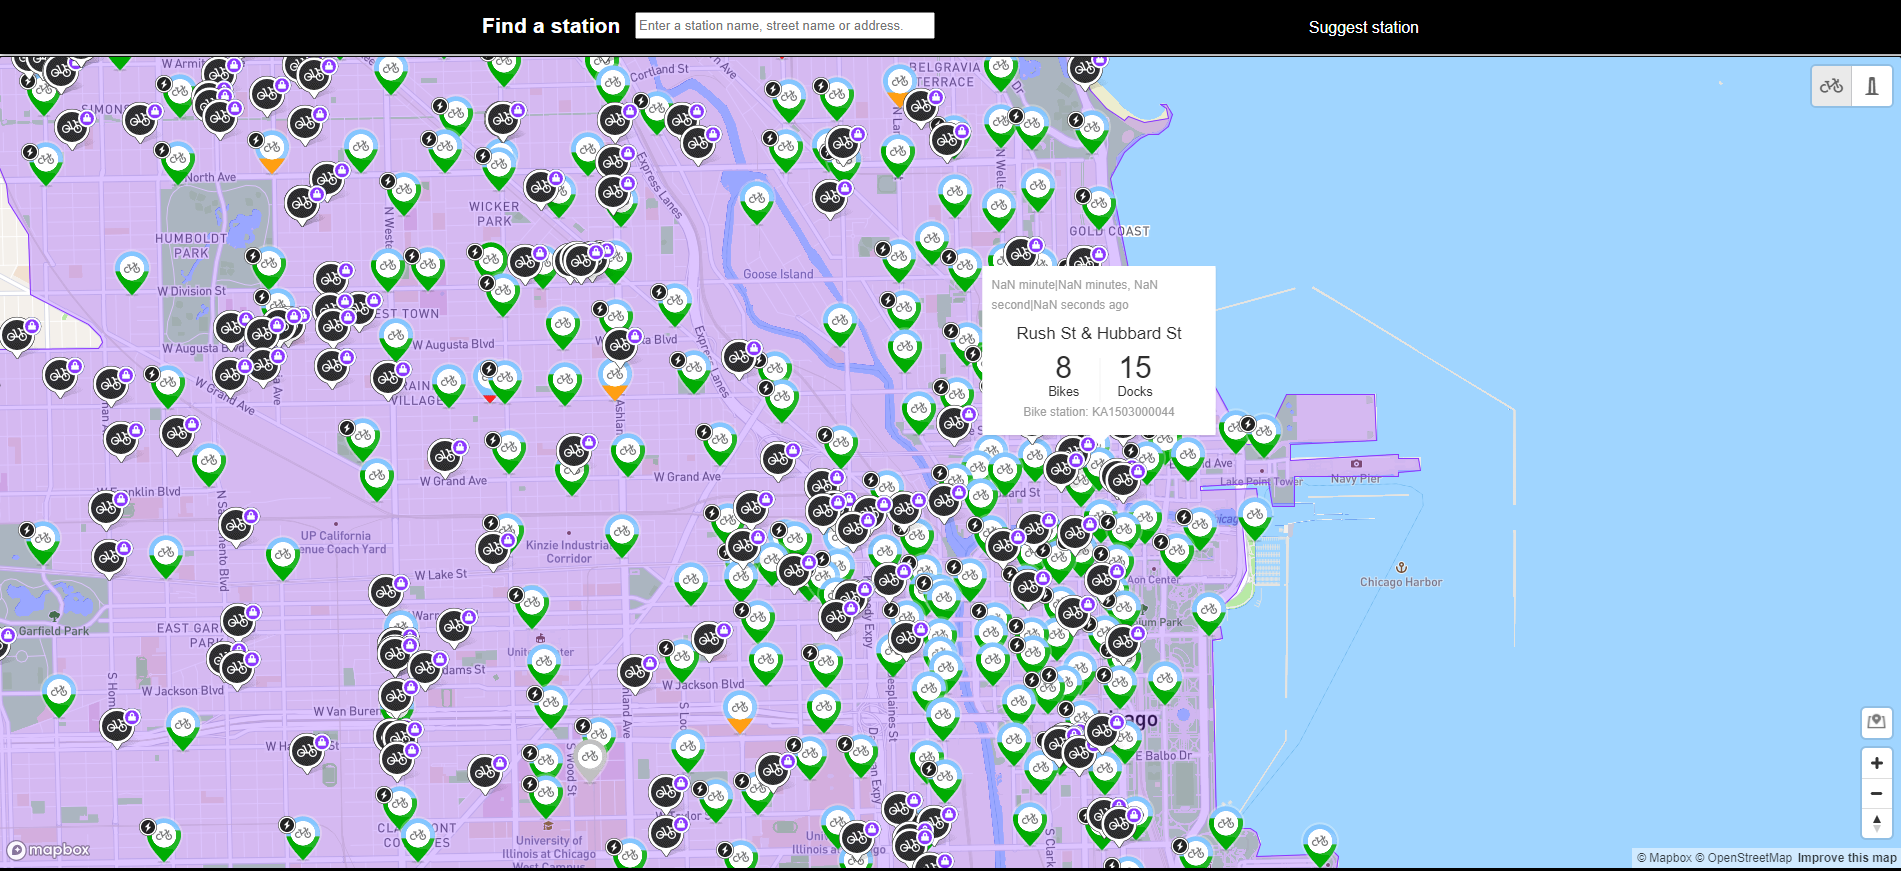
\includegraphics[width=14cm]{images/solution/preprocessing/divvy-map.png}
    \caption{Mapa interactivo de la red de estaciones de alquiler de biciletas en Chicago \cite{chicagomap}}
\end{figure}

\subsection{Preprocesado de datos}

Como bien se ha dicho en la anterior sección, se ha usado un \textit{dataset} público ofrecido por la compañía \textit{Divvy} \cite{divvy}. Este \textit{dataset} contiene el historial con todos los viajes registrados desde el 2004 al 2019 en la ciudad de Chicago. Estos datos se ofrecen divididos por partes: o bien por cuatrimestres o bien por meses. El \textit{dataset} final contiene $26.328.986$ de viajes y por cada viaje, se tienen 12 etiquetas asociados a ellos. En el Apéndice \ref{app:original_dataset} se puede ver una muestra de los datos recogidos en él.
\newline

Para el desarrollo de este proyecto, se han creado cuatro módulos distintos. Cada una de estos módulos tendrá como resultado una estructura de datos guardada en CSV a excepción del módulo del generado de ventanas que contendrán información que será útil para el siguiente módulo. El principal motivo de que los dos primeros módulos tengan como resultado la creación de un fichero es para ahorrar tiempo de cómputo innecesario cada vez que se quiera entrenar un modelo. Como para entrenar a los modelos es necesario multitud de pruebas con diferentes configuraciones, es un proceso que se hubiera repetido continuamente y cuyo resultado siempre hubiese sido el mismo. Por otro lado, el generador de ventanas, modulo que se explicará más adelante, al ser un módulo que es instantáneo y que además genera distintos resultados en función del modelo que se quiera desarrollar no guarda el resultado en algún archivo.


\begin{figure}[H]
    \centering
    
\includegraphics[width=16cm]{images/solution/modules/modules.png}
    \caption{Estructura del proyecto divida por módulos}
\end{figure}

Durante las siguientes secciones se explicarán cada uno de estos módulos en detalle incluyendo diagramas y código.


\subsubsection{\textit{Feature selection} - Unión de \textit{datasets} y filtro de variables}\label{feature-selection}

El \textit{dataset} original \cite{divvy} está divido en años y cada año en múltiples partes. Por lo tanto, la primera tarea de todas ha sido la unión de cada una de estas partes en un único fichero. El formato de archivo ofrecido por \textit{Divvy} es en un CSV como es normal, y por ello se ha usado principalmente la función \verb|read_csv| de pandas que convierte un CSV a un \verb|DataFrame|. Por otro lado, cada parte tenía su propia nomenclatura de columnas por lo que ha sido necesario crear una única nomenclatura para poder trabajar con un único fichero y por ello han sido renombradas algunas columnas. Una vez realizado el renombrado de columnas, el \verb|DataFrame| será anexionado a otro que contendrá todos los datos y que será el que se usará para los siguientes pasos.

\begin{displayquote}
"Un \verb|DataFrame| es una estructura de datos etiquetada en 2 dimensiones con columnas de tipos potencialmente diferentes. Se puede pensar en ello como una hoja de cálculo o una tabla SQL. Generalmente es el objeto más comúnmente usado en la librería de \textit{pandas}." \cite{pandas}
\end{displayquote}

Un ejemplo de \verb|DataFrame| que se ha visto con anterioridad podría ser la tabla \ref{tab:houses}. Para poder inicializar un \verb|DataFrame| se puede realizar desde un diccionario de Python, donde cada clave sea el \verb|string| que identifica a la columna y cada valor sea un vector con la misma cantidad de valores que filas quiere que se tenga. Otra forma de inicializar un \verb|DataFrame| es mediante el uso de funciones como \verb|read_csv()|, \verb|read_h5()| o \verb|read_pickle()|.
\newline

El código usado es algo parecido a lo que se muestra a continuación:

\begin{minted}[fontsize=\footnotesize]{python}
import pandas as pd

# Path to the csv files
csv_filenames = ["trips-2014-Q1", "trips-2014-Q2-Q3", 
                 "trips-2014-Q4", "trips-2015-Q1-Q2",
                 # ...
                 "trips-2019-Q3-Q4"]
csv_paths = [f"/path/to/{file}.csv" for file in csv_filenames]

# This will be the final DataFrame
df = pd.DataFrame()

# For every CSV do
for path in csv_paths:
    
    # CSV to DataFrame
    df_temp = pd.read_csv(path)
    
    # Parse date as datetime which is always first column
    df_temp[cols[0]] = pd.to_datetime(
        df_temp[cols[0]], 
        format='%Y-%m-%d %H:%M:%S',
        infer_datetime_format=True)
    
    # Rename the columns depending on their
    # current names with a external function
    df_temp = rename_columns(df_temp)
    
    # Merge the DataFrames
    df = pd.concat([df, df_temp], join='outer')

# ...
\end{minted}

Una vez obtenido la variable \verb|df| con todos los viajes, se necesita realizar un filtro de las columnas. En este punto, el \verb|DataFrame| contine 12 valores asociados a cada viaje.

\begin{minted}[fontsize=\footnotesize]{python}
df.columns

'''
Index(['trip_id', 'start_time', 'end_time', 'bikeid', 
       'tripduration', 'from_station_id', 
       'from_station_name', 'to_station_id',
       'to_station_name', 'usertype', 'gender',
       'birthyear'],
      dtype='object')
'''
\end{minted}

De este \verb|DataFrame| solo se seleccionan dos:

\begin{itemize}
    \item \textit{start\_time}: Este dato es necesario porque se quiere predecir el uso de bicicletas a partir de una información temporal. Este valor, dado en segundos usando el formato "Tiempo Unix" \cite{unix_time}, nos permite identificar en qué fecha y hora se inició el viaje. Gracias a ello, se pueden identificar distintos patrones, ya que estos varían durante la época del año. No existen los mismos patrones durante el invierno que durante el verano o incluso, no es lo mismo las 2 de la madrugada que las 2 de la tarde.
    \item \textit{from\_station\_id}: Los modelos que se van a construir predecirán el número de viajes que se inician en cada estación de Chicago de forma independiente. Este valor por tanto, será usado para calcular el número de viajes iniciados en un intervalo en cada estación.
\end{itemize}

El resto de atributos también son útiles para otro tipos de problemas como por ejemplo predecir el destino más probable en función de la estación donde se inicia el viaje, u obtener que conexiones son las más transitadas. Sin embargo, está fuera de los objetivos que se han planteado para este trabajo por lo que solo se usarán las columnas previamente mencionadas.
\newline
 
El dataset resultante por tanto, es el mismo dataset original pero con solo las columnas \textit{start\_time} y \textit{from\_station\_id}. En el código esto es fácil de implementar añadiendo solo la siguientes línea:
\begin{minted}[fontsize=\footnotesize]{python}
# ...
    
# Filter the columns that we need
cols = ["start_time", "from_station_id"]
df = df[cols]

# Save the DataFrame in a CSV
df.to_csv("trips.csv", index=False)
\end{minted}

Se podrían haber usado más columnas que ayudasen a la predicción, sin embargo, por falta de tiempo y porque los resultados obtenidos eran de por sí bastante buenos, no se ha visto la necesidad de añadirlos.
\newline

Gráficamente este módulo realiza lo siguiente:
\begin{figure}[H]
    \centering
    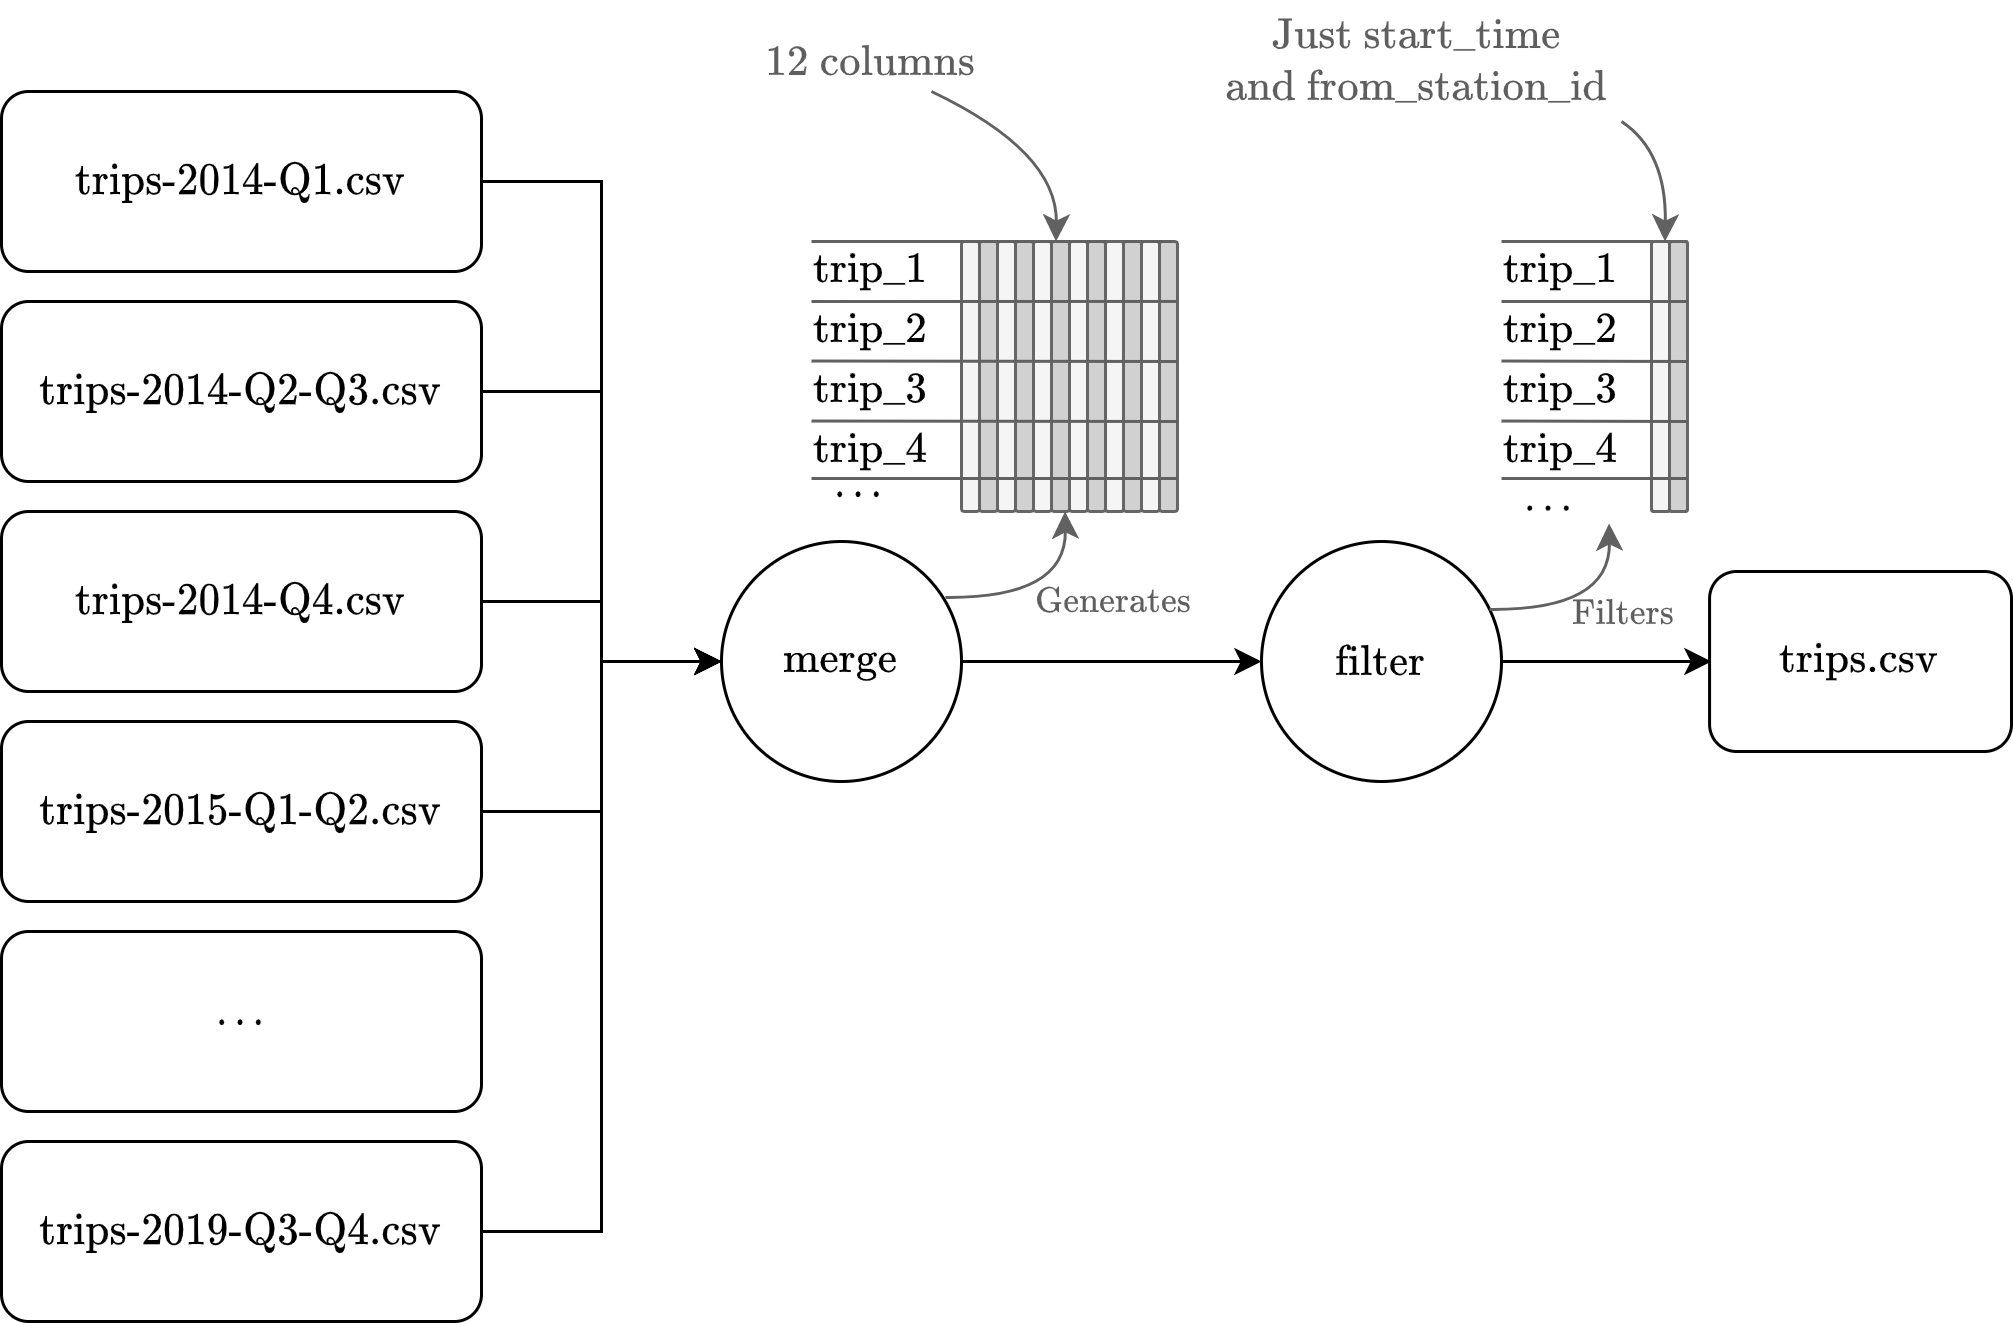
\includegraphics[width=12cm]{images/solution/modules/feature-selection.png}
    \caption{Estructura del módulo \textit{feature-selection}.}
\end{figure}
\subsubsection{Definición de entradas y salidas de las redes neuronales}\label{inputs-outputs}

Antes de continuar explicando los pasos llevados a cabo hay que diseñar que \textit{dataset} se necesita para entrenar a las redes neuronales. Uno de los principales requisitos en el diseño de redes neuronales es la correcta especificación del vector de entrada y salida de la red neuronal. La cantidad de variables y el tipo de variables que se usarán en la red es una de las principales claves para que el modelo funcione de forma satisfactoria. En este apartado se explicará tanto la estructura del vector de entrada como la estructura del vector de salida acompañado de ejemplos gráficos.
\newline

Los modelos con los que trabajaremos tendrán como entrada valores que representan la fecha y la hora representados con los siguientes atributos: \textit{hour} (h), \textit{day\_of\_week}(d) y \textit{month}(m). Es decir, los viajes se agruparan por intervalos, creando de este modo una nueva columna que se denominará \textit{quantity\_$j$} (q), siendo $j$, el índice de la estación. En total hay $633$ estaciones en la ciudad de Chicago. Por lo que para cada intervalo, la red neuronal contará con $636$ valores de entrada. Se pueden ver ejemplos gráficos en la Figura \ref{fig:models-design-1} y \ref{fig:models-design-2}.
\newline

Si se quiere usar más intervalos para que la red entrene, el vector resultante tendrá un número de elementos múltiplo de $636$. Por ejemplo, si se quieren usar 5 intervalos como vector de entrada, entonces la red tendrá una primera capa con $636 \times 5 = 3180$ unidades o neuronas. Por otro lado, se podrían usar más variables conteniendo información importante como puede ser el calendario laboral o variables relacionadas con la meteorología, las cuales influyen en los patrones de comportamiento de la red de bicicletas.
\newline

Por ejemplo, un lunes no laboral, la cantidad de bicicletas alquiladas en un parque será mayor que cualquier otro lunes de otra semana. U otro ejemplo, si un día las condiciones meteorológicas nos son favorables para el uso de bicicleta, la cantidad de bicicletas alquiladas se reducirán considerablemente. Este tipo de variables son algún ejemplo que se podría añadir al \textit{dataset} y así poder mejorar la precisión del modelo pero por falta de tiempo y por simplicidad no se han añadido. Además, los resultados obtenidos de por sí se han considerado bastante buenos y por lo tanto, no se ha visto la necesidad de invertir tiempo en este apartado aunque sería un buen estudio como mejoraría estos modelos con dichos cambios.
\newline

Por otra parte, la salida de la red será un vector que contenga la predicción para todas las estaciones de la red. Es decir, se calculará un vector donde cada valor será la predicción de alguna de las estaciones de la red en un intervalo en concreto. La longitud del vector por lo tanto vendrá dado por el número de estaciones con las que se trabaje, que en total son $633$ multiplicado por la cantidad de intervalos que se quieren predecir, es decir, el vector resultante tendrá $633 \times \text{n\_stations}$ valores. 
\newline

En los modelos autoregresivos, a pesar de ser modelos capaces de predecir múltiples intervalos si fuese neceario, la salida de estos modelos siempre serán de un intervalo. Esto es debido a que es necesario calcular todos los intervalos de forma independiente pues el modelo autoregresivo usa su propia predicción como vector de entrada. Se puede ver más información sobre esto en la Sección \ref{window_ar} y \ref{model_ar}.
\newline

A continuación, se pueden ver gráficamente varios ejemplos de distintas configuraciones de red usando diferentes combinaciones para la cantidad de intervalos de entrada y salida:


\begin{figure}[H]
    \centering
    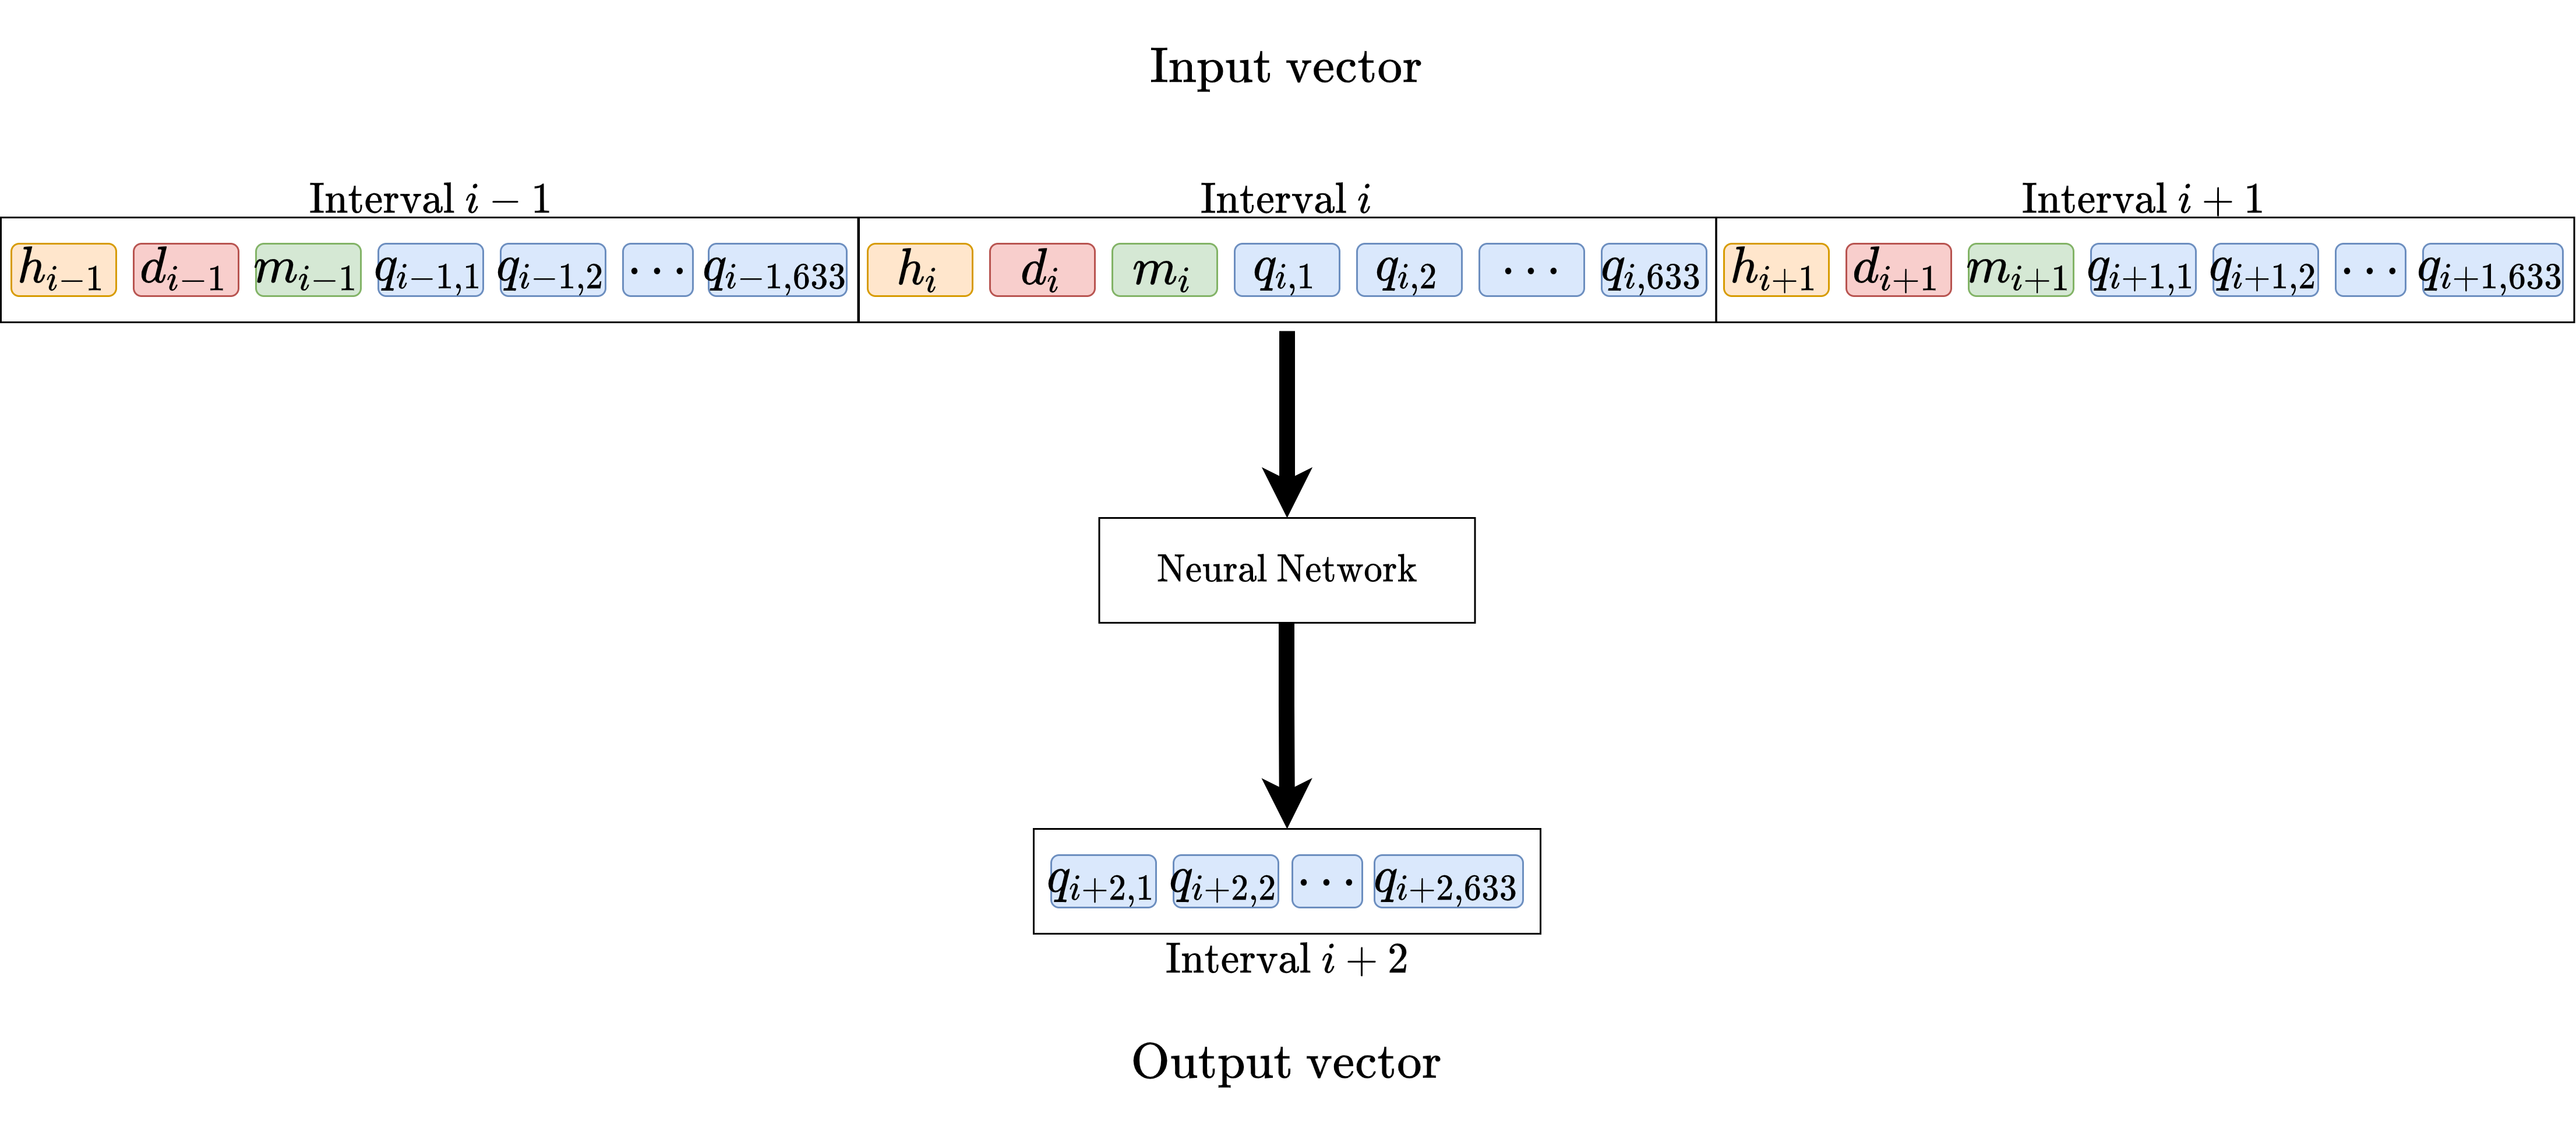
\includegraphics[width=14cm]{images/solution/preprocessing/models-design-1.png}
    \caption{Ejemplo de red neuronal que usa 3 intervalos de entrada y predice 1 intervalo}
    \label{fig:models-design-1}
\end{figure}

\begin{figure}[H]
    \centering
    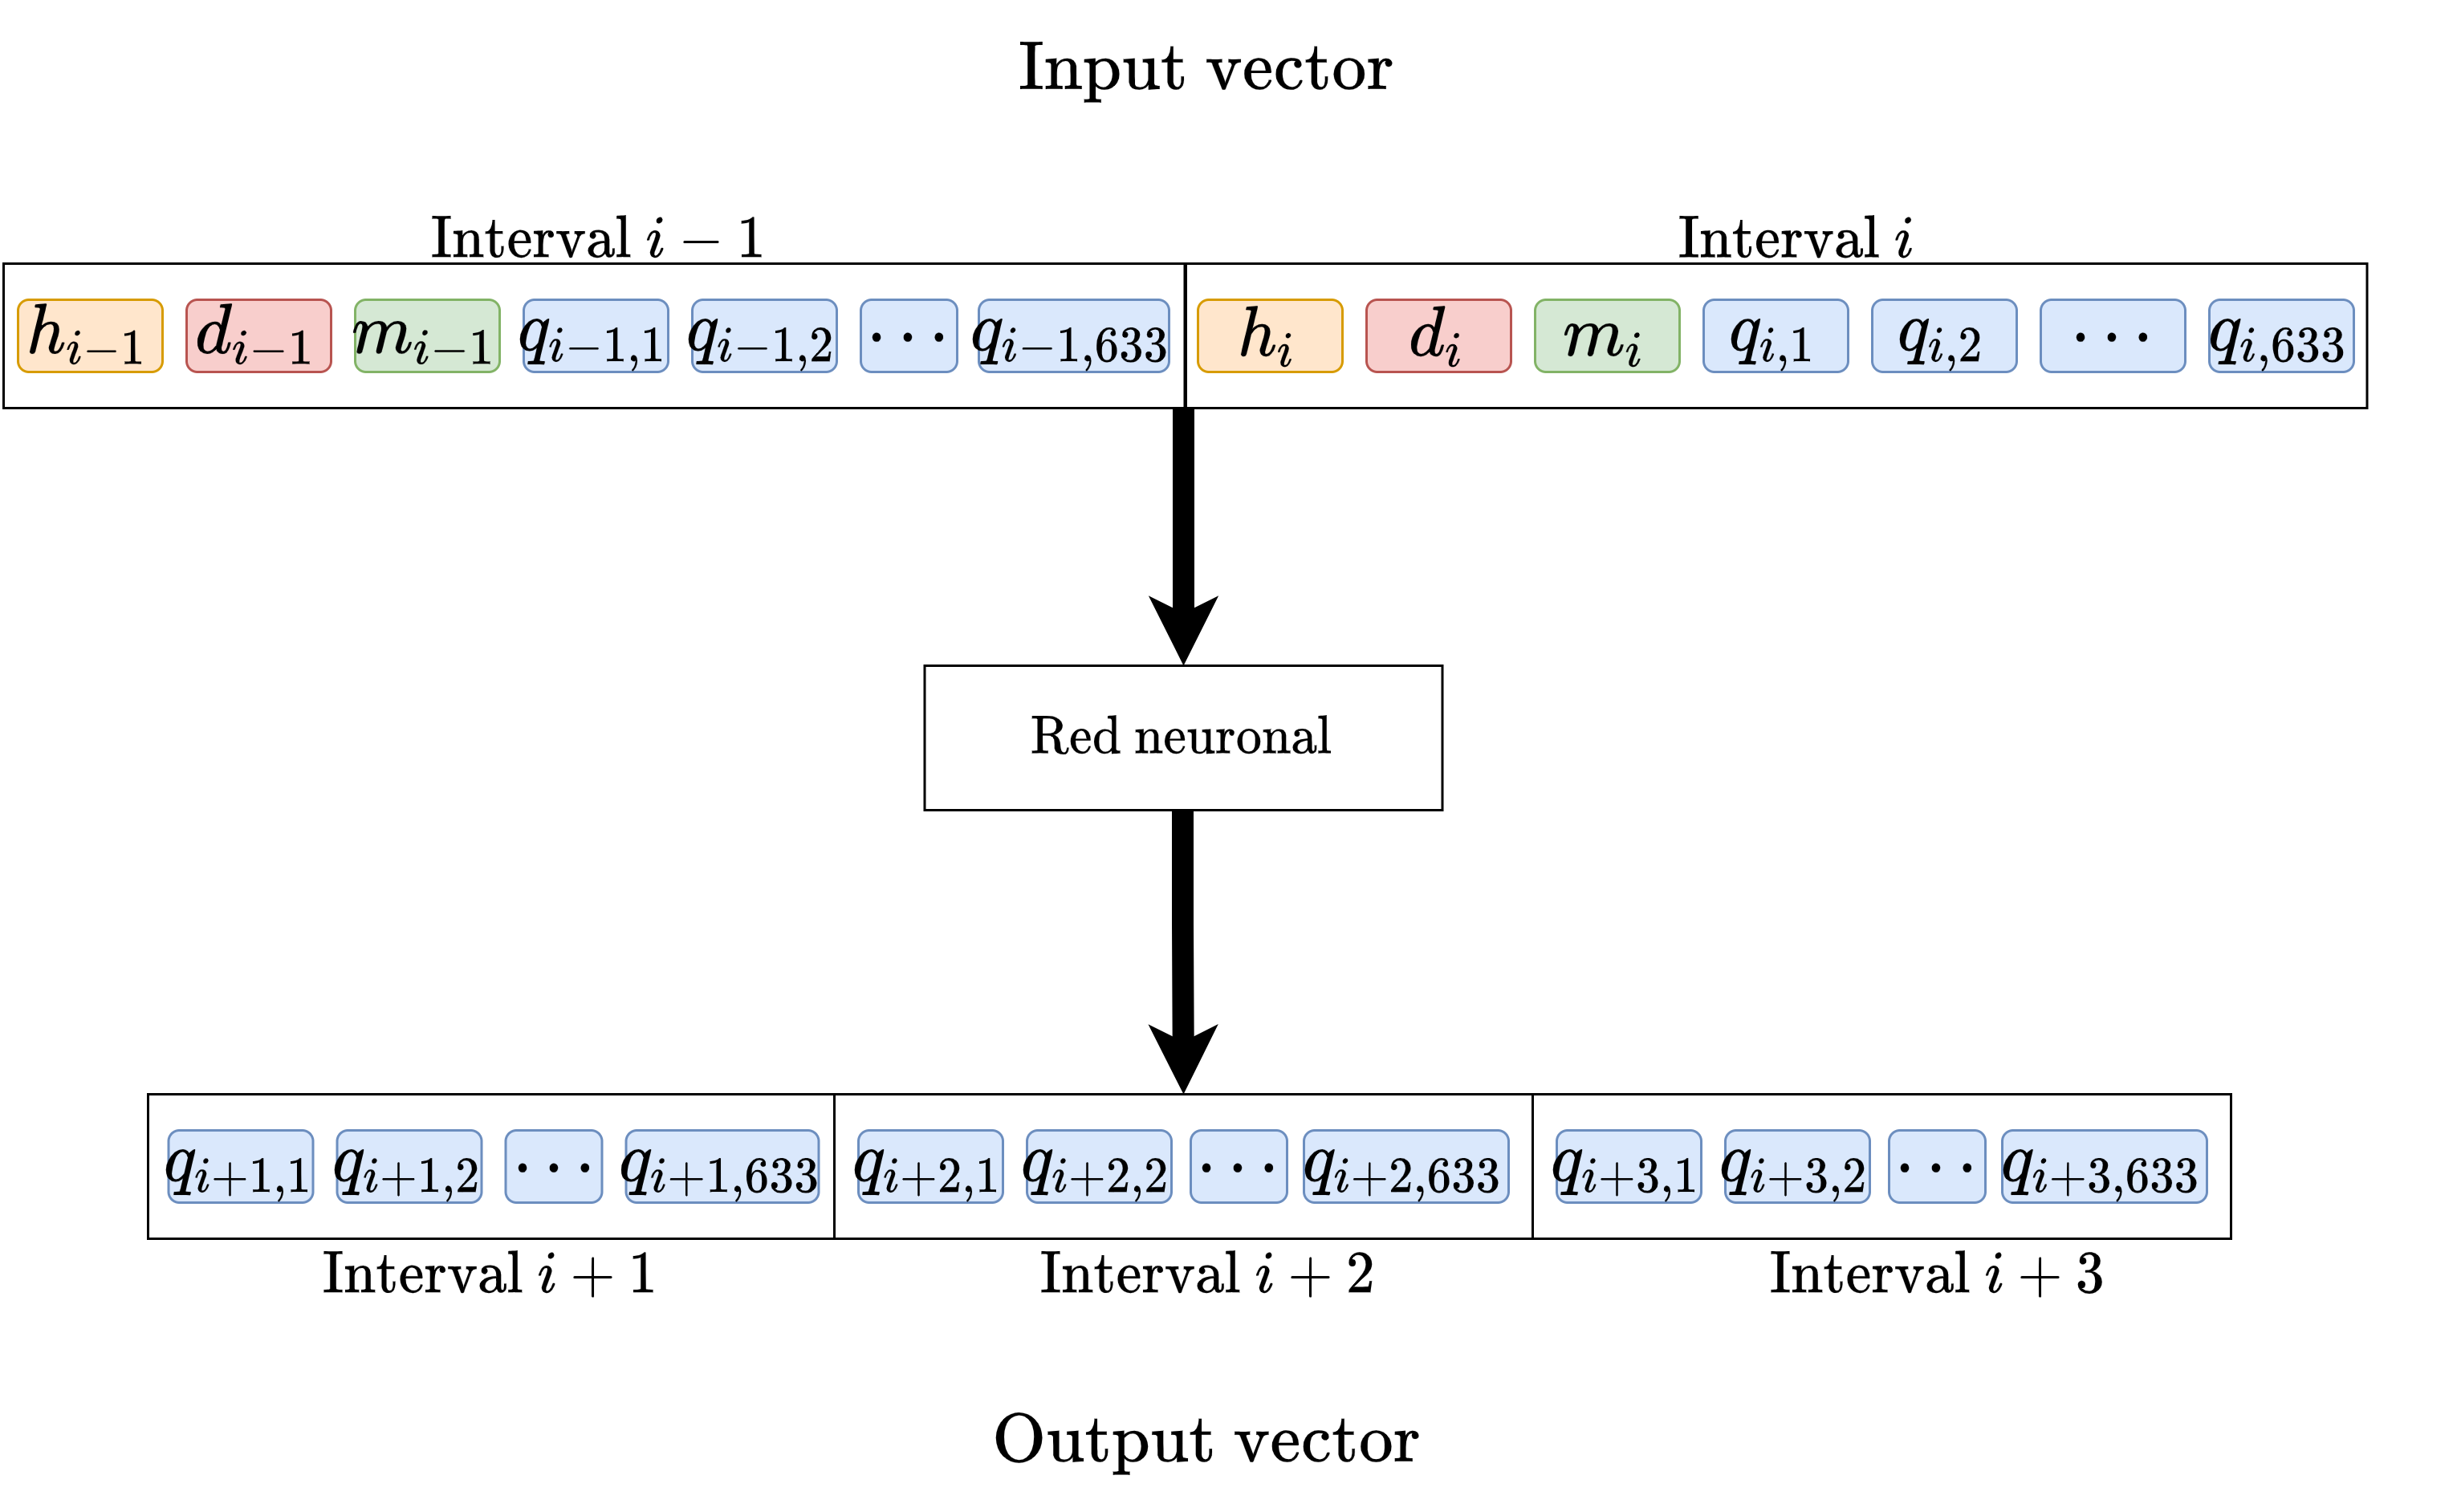
\includegraphics[width=14cm]{images/solution/preprocessing/models-design-2.png}
    \caption{Ejemplo de red neuronal que usa 2 intervalos de entrada y predice 3 intervalos}
        \label{fig:models-design-2}
\end{figure}



Esta estructura, nos permite trabajar con un número variable de estaciones siendo los modelos fácilmente exportables a otras ciudades y otras redes donde la cantidad de estaciones sea distinta. O incluso, si se quisiese trabajar con una única estación se podría realizar sin ningún problema, puesto que cada estación es representada con su propia columna. El código desarrollado para que los modelos funcionen es fácilmente reutilizable para un conjunto de estaciones más pequeñas u otras ciudades o incluso otros problemas de la misma índole, solo haría falta modificar el módulo de \textit{feature-selection} y preprocesamiento.

\subsubsection{Modificando el \textit{dataset} para la red neuronal}\label{dataset-creation}

El \textit{dataset} que se tiene en este punto es un \textit{dataset} que tiene tantas filas como viajes haya habido entre el 2014 y 2019. Por cada fila, se tienen dos atributos: \textit{from\_station\_id} y \textit{start\_time}. 
\newline

En este módulo se quiere modificar dicho \textit{dataset} para obtener un \textit{dataset} que contenga los vectores que puedan ser usados como vectores de entrada en la red. Es decir, se quiere crear un \textit{dataset} que contenga en cada fila los intervalos y en cada columna los datos de dicho intervalo: \textit{hour}, \textit{day\_of\_week}, \textit{month} y \textit{quantity\_$j$}. Al finalizar todos los pasos de este módulo, los datos se guardarán en un archivo llamado \small{\verb|intervals.csv|} y se puede ver una muestra de estos datos en el Apéndice \ref{app:intervals_dataset}.
\newline

Primeramente, el código de este módulo, carga los datos del anterior módulo del archivo CSV \small{\verb|trips.csv|}:
\begin{minted}[fontsize=\footnotesize]{python}
import pandas as pd

# Read CSV as DataFrame an use datetime as index
df = pd.read_csv("/path/to/trips.csv", index="start_time")
\end{minted}

Para poder obtener este dataset, se han tenido que programar una serie de pasos:
\begin{enumerate}
    \item \underline{Agrupar los viajes por intervalos}: Este paso tiene como objetivo agrupar la cantidad de viajes que se inician en cada una de las estaciones en intervalos. Se han estudiado diferentes tamaños de intervalos, como por ejemplo, intervalos de 15 ó 30 minutos, pero finalmente, se ha elegido 1 hora porque se reduce de forma considerable la cantidad de datos y sigue siendo un intervalo válido y no muy amplio.
    \newline
    
    Para este paso lo que se ha realizado ha sido agrupar los distintos viajes en intervalos en función de la columna \textit{from\_station\_id} y \textit{start\_time}. Por ejemplo, teniendo el siguiente \textit{dataset} quese puede ver en la Tabla \ref{tab:starttime_withsid} que contiene ejemplos de viajes, se quiere obtener otro que agrupe por tiempo y por estación como se puede ver en el Tabla \ref{tab:intervals_example}. Para ello primero se agrupara por estación y por intervalo y en el siguiente paso se pivotarán para convertir filas a columnas.
    \newline
    
    Como ejemplo, supongamos que en la variable \small{\verb|df|} se tiene el siguiente \small{\verb|DataFrame|}:

    \begin{table}[H]
    \footnotesize
    \centering
    \begin{tabular}{c|rr}
        \toprule
          \textit{start\_time} & \textit{from\_station\_id}  \\
        \midrule
        
        10:10 - 12/2/2018 & 48\\
        10:28 - 12/2/2018 & 15\\
        10:56 - 12/2/2018 & 15\\
        11:03 - 15/2/2018 & 15\\
        11:12 - 15/2/2018 & 48\\
        11:15 - 15/2/2018 & 15\\
        11:18 - 15/2/2018 & 15\\
        11:31 - 15/2/2018 & 15\\
        11:44 - 15/2/2018 & 48\\
        11:49 - 15/2/2018 & 15\\
        22:00 - 16/2/2018 & 15\\
        22:15 - 16/2/2018 & 48\\
        22:37 - 16/2/2018 & 193\\
        22:56 - 16/2/2018 & 48\\
        \bottomrule
        
    \end{tabular}
    \cprotect\caption{Ejemplo de \textit{dataset} original de \textit{Divvy} que está en \small{\verb|trips.csv|}}
    \label{tab:starttime_withsid}
    \end{table}
    
    Se deben de agrupar los viajes por estación, usando \small{\verb|group_by()|},  \small{\verb|resample()|} y \small{\verb|size()|}. Se puede conseguir esta agrupación usando las siguientes líneas de código:
    
    \begin{minted}[fontsize=\footnotesize]{python}
INTERVAL = "1H"  # It could be also 15Min

df = df.groupby('from_station_id') \
       .resample(INTERVAL, on='start_time') \
       .size() \    # Resampling using the sum rule
       .to_frame()  # Converts it to DataFrame
    \end{minted}
    
    El resultado de este proceso usando el ejemplo de tabla \ref{tab:starttime_withsid} se puede ver en la siguiente tabla:
    
    \begin{table}[H]
    \footnotesize
    \centering
    \begin{tabular}{c|rr}
        \toprule
          \textit{start\_time} & \textit{from\_station\_id} & \textit{quantity}  \\
        \midrule
        
        10:00 - 12/2/2018 & 15 & 2\\
        10:00 - 12/2/2018 & 48 & 1\\
        10:00 - 12/2/2018 & 193 & 0\\
        11:00 - 15/2/2018 & 15 & 5\\
        11:00 - 15/2/2018 & 48 & 2\\
        11:00 - 15/2/2018 & 193 & 0\\
        22:00 - 16/2/2018 & 15 & 1\\
        22:00 - 16/2/2018 & 48 & 2\\
        22:00 - 16/2/2018 & 193 & 1\\
        \bottomrule
    \end{tabular}
    \cprotect\caption{Ejemplo del \textit{dataset} agrupados por estaciones y por intervalos.}
    \label{tab:justintervals}
    \end{table}
    
    

    \item \underline{Pivotar por intervalos}: Este paso tiene como objetivo agrupar todos los intervalos en uno solo, aumentando por tanto la cantidad de columnas reduciendo la cantidad de filas. Es decir, se quiere tener que por cada fila represente un intervalo y por cada columna una estación. Usando el mismo ejemplo del paso anterior, el \small{\verb|DataFrame|} final quedaría de la siguiente manera:
    \begin{table}[H]
    \footnotesize
    \centering
    \begin{tabular}{c|rrr}
        \toprule
        \textit{start\_time} & \textit{quantity\_15} & \textit{quantity\_48} & \textit{quantity\_193}  \\
        \midrule
        10:00 - 12/2/2018 & 2 & 1 & 0 \\
        11:00 - 15/2/2018 & 5 & 2 & 0 \\
        22:00 - 16/2/2018 & 1 & 2 & 1 \\
        
        \bottomrule
    \end{tabular}
    \cprotect\caption{Ejemplo de \textit{dataset} que contiene los intervalos.}
    \label{tab:intervals_example}
    \end{table}
    
    Principalemente, el código usado para este paso hace uso de la función de \textit{pandas} denominada \small{\verb|pivot()|}:
    \begin{minted}[fontsize=\footnotesize]{python}
# Prepare the new columns names for each station
df["quantity_index"] = "quantity_" + \
                        df["from_station_id"].astype("str")

# We don't need from_station_id anymore
df = df.drop(columns=["from_station_id"])

# Make the pivot around quantity_index column and
# set the value of the column the same value as
# quantity from before saving quantity from
df = df.pivot(columns='quantity_index', values='quantity')

# If station any interval didn't have any trips for
# a station, then fill it with 0
return df.fillna(0)
    \end{minted}
    
    \item \underline{Obtener la variables de tiempo}: La columna \textit{start\_time} es una lista con \textit{timestamps} y por lo tanto tiene información más de la necesaria (año, mes, día, hora, minuto, segundo...). La única información temporal que se necesita son un subconjunto de dichos valores. En concreto de los valores que se han creído ser útiles son: la hora, el día de la semana (no es lo mismo un lunes que un sábado) y el mes (no es lo mismo un mes de invierno que de verano). Estos son los valores más simples que se han usado pero eso no quita que se puedan usar otros datos que aportan más información como por ejemplo: día del mes, año o el minuto. 
    \newline
    
    Usando las variables de esta forma y no pasando el \textit{timestamp} directamente a la red, el modelo puede aprender patrones en función de variables más simples como la hora, el día de la semana o el mes, y no con un número de 64 bits que apenas aporta información alguna puesto que la red lo tomaría como valores ascendentes sin ningún tipo de criterio.
    
    Para crear las nuevas columnas con los atributos que se han explicado anteriormente se han usado las siguientes líneas de código:
    \begin{minted}[fontsize=\footnotesize]{python}
# Index and start_time column is the same

df['hour'] = df.index.hour              # Number between 0-23
df['day_of_week'] = df.index.dayofweek  # Number between 0-6
df['month'] = df.index.month            # Number between 1-12
    \end{minted}
    
    Al final de este paso existirán por tanto las siguientes columnas para cada uno de los intervalos: \textit{start\_time}, \textit{hour}, \textit{day\_of\_week}, \textit{month} y una columna por cada estación. La columna \textit{start\_time} no se borra pues es la columna usada como índice y ayuda a la hora de entender la información con la que se trabaja. Pero no será usada por la red neuronal.
    \newline
    
    Usando el mismo ejemplo que los pasos anteriores, la tabla quedaría de la siguiente manera:
    \begin{table}[H]
    \footnotesize
    \centering
    \begin{tabular}{c|rrr|rrr}
        \toprule
        \textit{start\_time} & \textit{quantity\_15} & \textit{quantity\_48} & \textit{quantity\_193} & \textit{hour} & \textit{day\_of\_week} & \textit{month} \\
        \midrule
        10:00 - 12/2/2018 & 2 & 1 & 0 & 10 & 0 & 2 \\
        11:00 - 15/2/2018 & 5 & 2 & 0 & 11 & 3 & 2 \\
        22:00 - 16/2/2018 & 1 & 2 & 1 & 22 & 4 & 2 \\
        
        \bottomrule
    \end{tabular}
    \cprotect\caption{Ejemplo de \textit{dataset} final que será usada por la red neuronal.}
    \label{tab:intervals_example}
    \end{table}
    
    
    En este punto también se estudió la posibilidad de guardar la información de las variables temporales en forma de señal con valores entre los rangos $[-1, 1]$ usando seno y coseno \cite{reddit_time}. Esto permite que el modelo tenga acceso a la información temporal con valores continuos y no discretos como se puede ver en la figura \ref{fig:hour-stepvssignal} a continuación. Los resultados que se obtuvieron con ambas técnicas fueron similares, por lo que por simplicidad se dejo con valores discretos.
    
   \begin{figure}[H]
  \centering
  \subfloat[Hora con valores continuos de $-1$ a $1$]{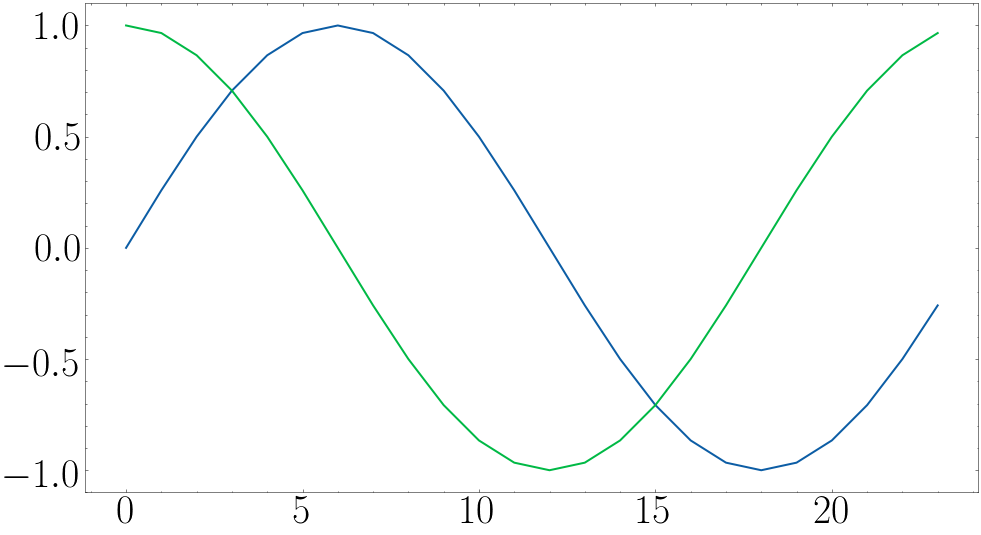
\includegraphics[width=0.4\textwidth]{images/solution/modules/hour_signal.png}\label{fig:f1}}
  \hfill
  \subfloat[Hora con valores discretos de $0$ a $23$]{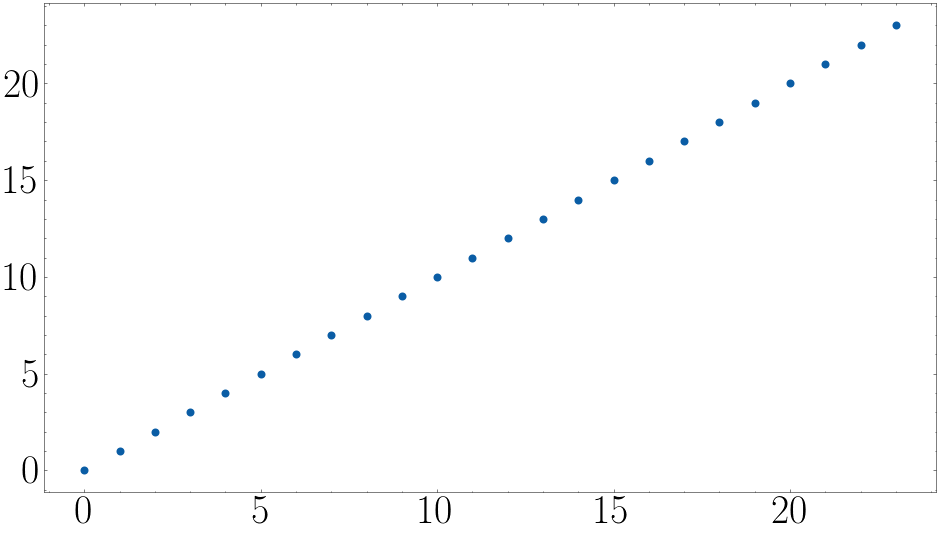
\includegraphics[width=0.4\textwidth]{images/solution/modules/hour_steps.png}\label{fig:f2}}
  \caption{Posibles formas de representar la variable \textit{hour}.}
  \label{fig:hour-stepvssignal}
\end{figure}
    
\end{enumerate}


El \small{\verb|DataFrame|} obtenido por este módulo se guarda en un fichero CSV llamado \small{\verb|intervals.csv|} que será usado por los siguientes módulos cuyo contenido tendrá una estructura similar a la que se muestra en la Tabla \ref{tab:intervals_example}.

\begin{minted}[fontsize=\footnotesize]{python}
# Save df in a CSV file
df.to_csv("path/to/intervals.csv")
\end{minted}
\subsection{Generador de ventanas}\label{window-generator}

El primer paso de este módulo es cargar el \small{\verb|DataFrame|} generado en el anterior paso y dividirlo en tres partes: entrenamiento, validación y test. En concreto se han usado los datos del año 2017 para el entrenamiento, los datos del 2018 para la validación y los datos del 2019 para el test. A continuación se muestran las líneas de código usadas que realiza dicha división:
\begin{minted}[fontsize=\footnotesize]{python}
from datime import datetime


def small_dataset(df, from_date, to_date):
    sub_df = df[(df.index >= from_date) & (df.index <= to_date)]
    
    # Just making sure intervals are sorted
    sub_df = sub_df.sort_values(by="start_time") 
    
    return sub_df


'''
Splits the df into 3 parts depending on the year of the input
'''
def split_dataset(df, train_year=2017, validation_year=2018,
                      test_year=2019):
    dfs = []
    
    for year in [train_year, validation_year, test_year]:
        # 1st of Jan at 00:00
        from_date = datetime(year, 1, 1, 0)           
        
        # 31st of Dec at 23:59
        to_date = datetime(year, 12, 31, 23, 59, 59)
        
        dfs.append(small_dataset(df, from_date, to_date))

    return dfs
    
df = pd.read_csv("/path/to/intervals.csv")
train_df, val_df, test_df = split_dataset(df)
\end{minted}
Estas tres variables (\small\verb|train_df|, \small\verb|val_df| y \small\verb|test_df|) serán usadas para las distintas fases que tiene el entrenamiento de una red neuronal como se ha explicado en la sección \ref{training}.
\newline

El módulo de generador de ventanas está basado en el código de un tutorial oficial de la librería de Tensorflow \cite{windowgenerator}. Básicamente este generador permite agrupar los intervalos de forma variable y permite ajustar al modelo a las necesidades que se necesiten. Los modelos de este trabajo harán un conjunto de predicciones basadas en una ventana de muestras consecutivas de los datos. Principalmente la ventana se puede ajustar con tres variables:

\begin{itemize}
    \item Número de intervalos de entrada (\textit{inputs}): Permite establecer la cantidad de intervalos que tendrá el modelo como valores de entrada. En este trabajo como se ha explicado en la anterior sección se está usando un intervalo de un hora. Por lo que si se quiere que el modelo tenga datos un día previo para predecir, indicaremos al modelo que se quiere tener 24 intervalos previos. Hay que recalcar que es sumamente importante que los datos de la ventana estén ordenados y que sean intervalos contiguos.
    \newline
    
    \item Número de intervalos de salida (\textit{labels}): Permite establecer la cantidad de intervalos que se quieren predecir, es decir, la cantidad de intervalos que el modelo devolverá. En este trabajo por cada modelo se han probado distintas configuraciones cuyos resultados se mostrarán más adelante. Cabe destacar que cuánto mayor sea este valor y por lo tanto mayor cantidad de predicciones que el modelo realizará, el modelo se espera que sea menos preciso. Se denomina \textit{labels} (etiquetas en español), puesto que son los intervalos que se van a usar para predecir las etiquetas de \textit{quantity}.
    \newline
    
    \item Desplazamiento (\textit{offset}): Es una variable que permite establecer un valor entre los datos de entrada y los datos de salida. Esto es útil porque se puede preparar modelos que dados 24 intervalos de entrada, por ejemplo, se intente prever el mismo intervalo pero de un día futuro.
\end{itemize}

A continuación se muestran algunos ejemplos de ventanas con distintas configuraciones.:

\begin{figure}[H]
    \centering
    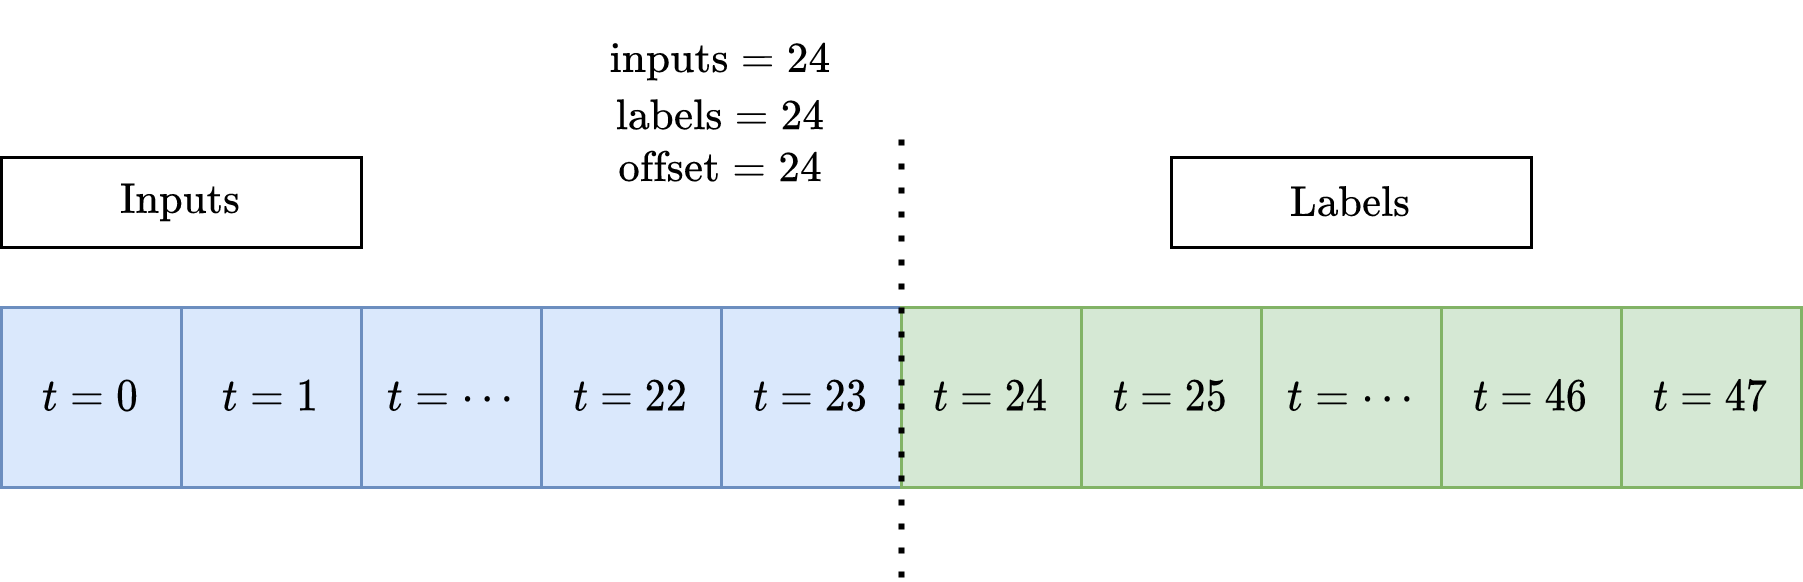
\includegraphics[width=12cm]{images/solution/modules/windows/windows-1.png}
    \caption{Ventana con un múltiples entradas y múltiples salidas}
\end{figure}


\begin{figure}[H]
    \centering
    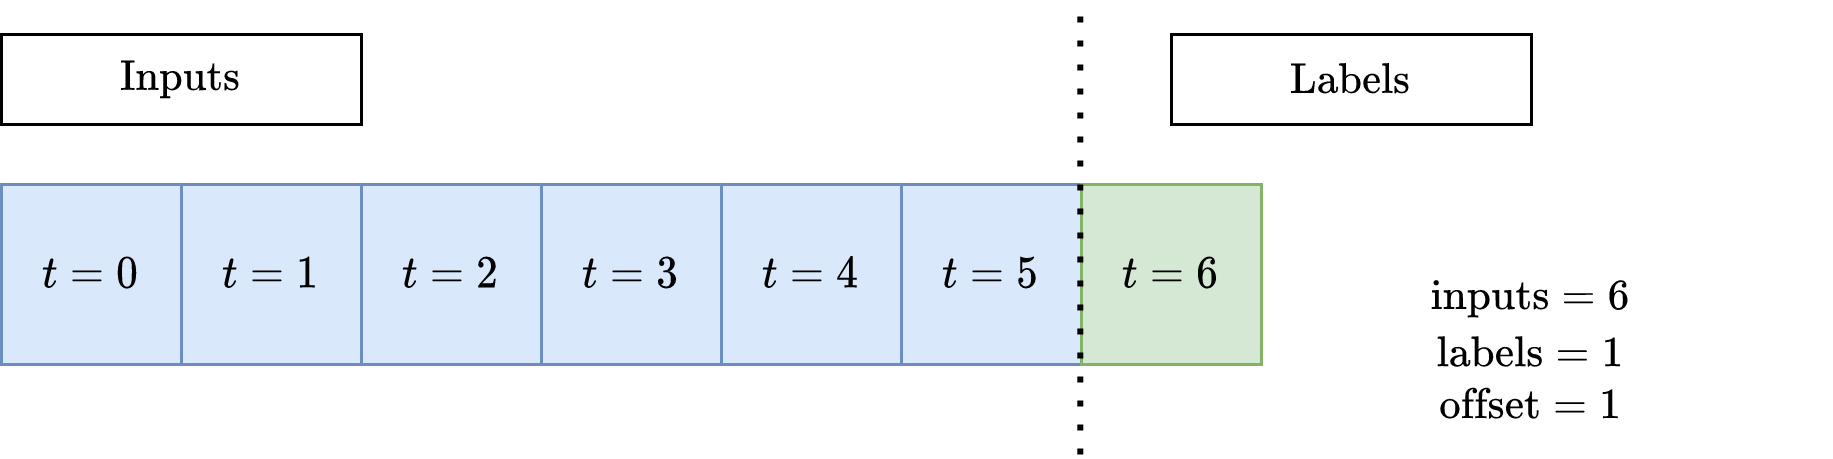
\includegraphics[width=12cm]{images/solution/modules/windows/windows-2.png}
    \caption{Ventana con un único intervalo de salida}
\end{figure}



\begin{figure}[H]
    \centering
    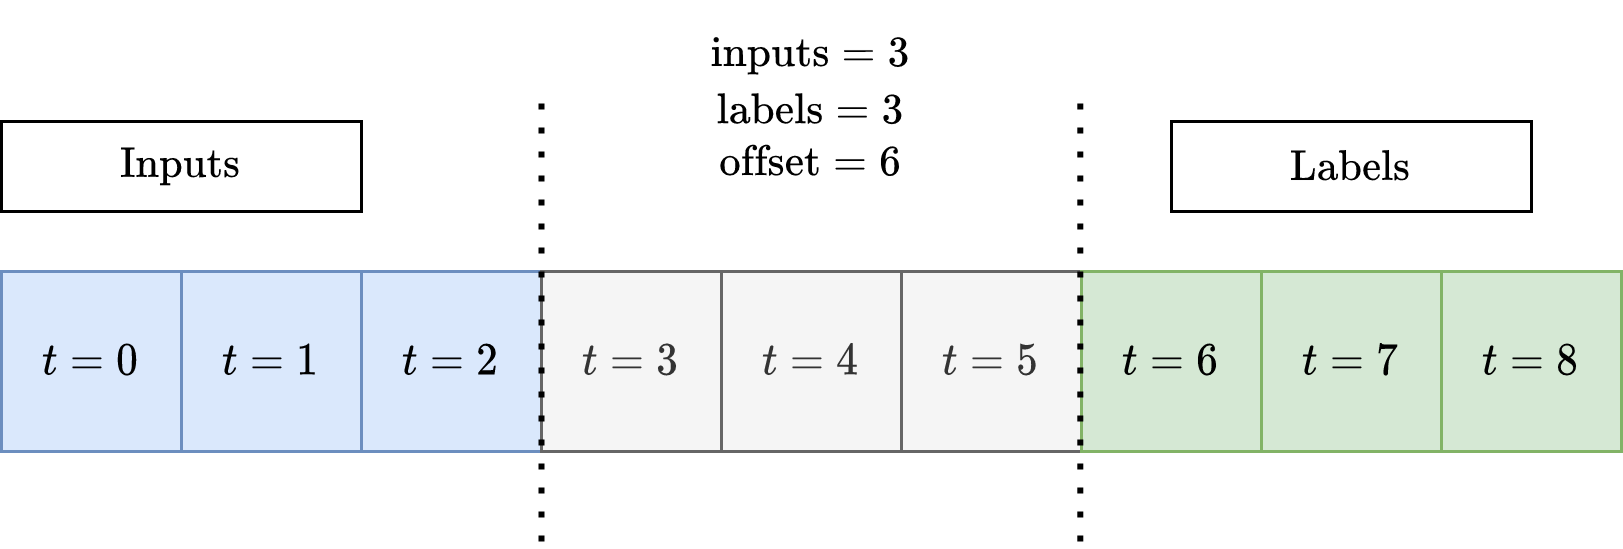
\includegraphics[width=12cm]{images/solution/modules/windows/windows-3.png}
    \caption{Ventana con \textit{offset}}
\end{figure}

Las cajas representan intervalos. El color azul representa que serán intervalos que el modelo usará como de entrada, es decir, cada caja azul tiene asociado un vector con \textit{hour}, \textit{day\_of\_week}, \textit{month} y la cantidad de viajes iniciados para todas las estaciones en dicho intervalo. Esto, como se ha explicado en la sección \ref{inputs-outputs}, se transformará en un vector de una única dimensión. Las cajas verdes por otro lado representa los intervalos que la red va las redes neuronales van a predecir. Por cada intervalo se creará un vector con tantos elementos como estaciones haya en el sistema siendo cada valor la predicción para cada estación. Como se verá más adelante, en las redes se incluirá una capa que permite la transformación de un vector a una matriz con lo que se conseguirá que la salida de las redes neuronales sea una matriz, donde cada fila es un intervalo y cada columna es una estación y cuyos valores serán las predicciones.
\newline


Las predicciones por otro lado se pueden realizar de dos formas distintas:

\begin{itemize}
    \item Predicción única: Dado un conjunto de datos de entrada se realizarán todas las predicciones a partir de esos datos.
    
    \begin{figure}[H]
    \centering
    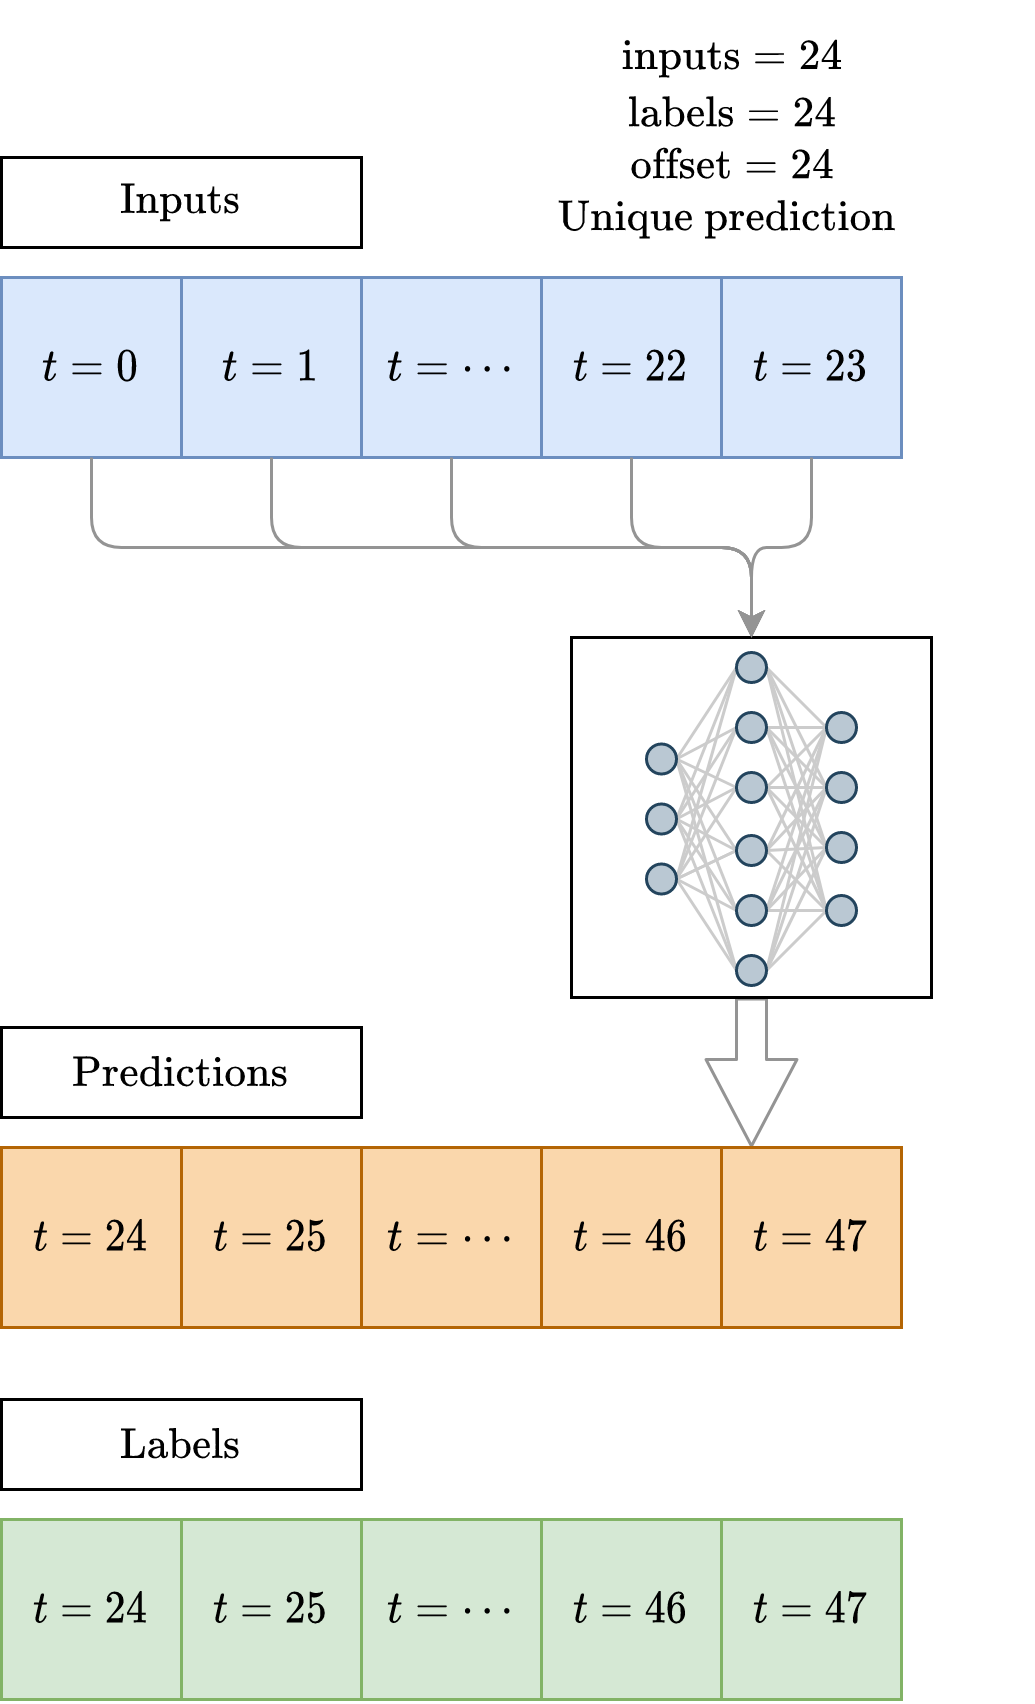
\includegraphics[width=7cm]{images/solution/modules/windows/windows-predictions-one-shot.png}
    \caption{Predicciones únicas}
    \end{figure}

    \item Predicción auto-regresiva \label{window_ar}: Se realizará primero la predicción más próxima en el futuro. Dicho valor será usado junto con el resto de valores de entrada (excepto el intervalo más pasado) para poder calcular la siguiente predicción. Visto gráficamente:
    \begin{figure}[H]
    \centering
    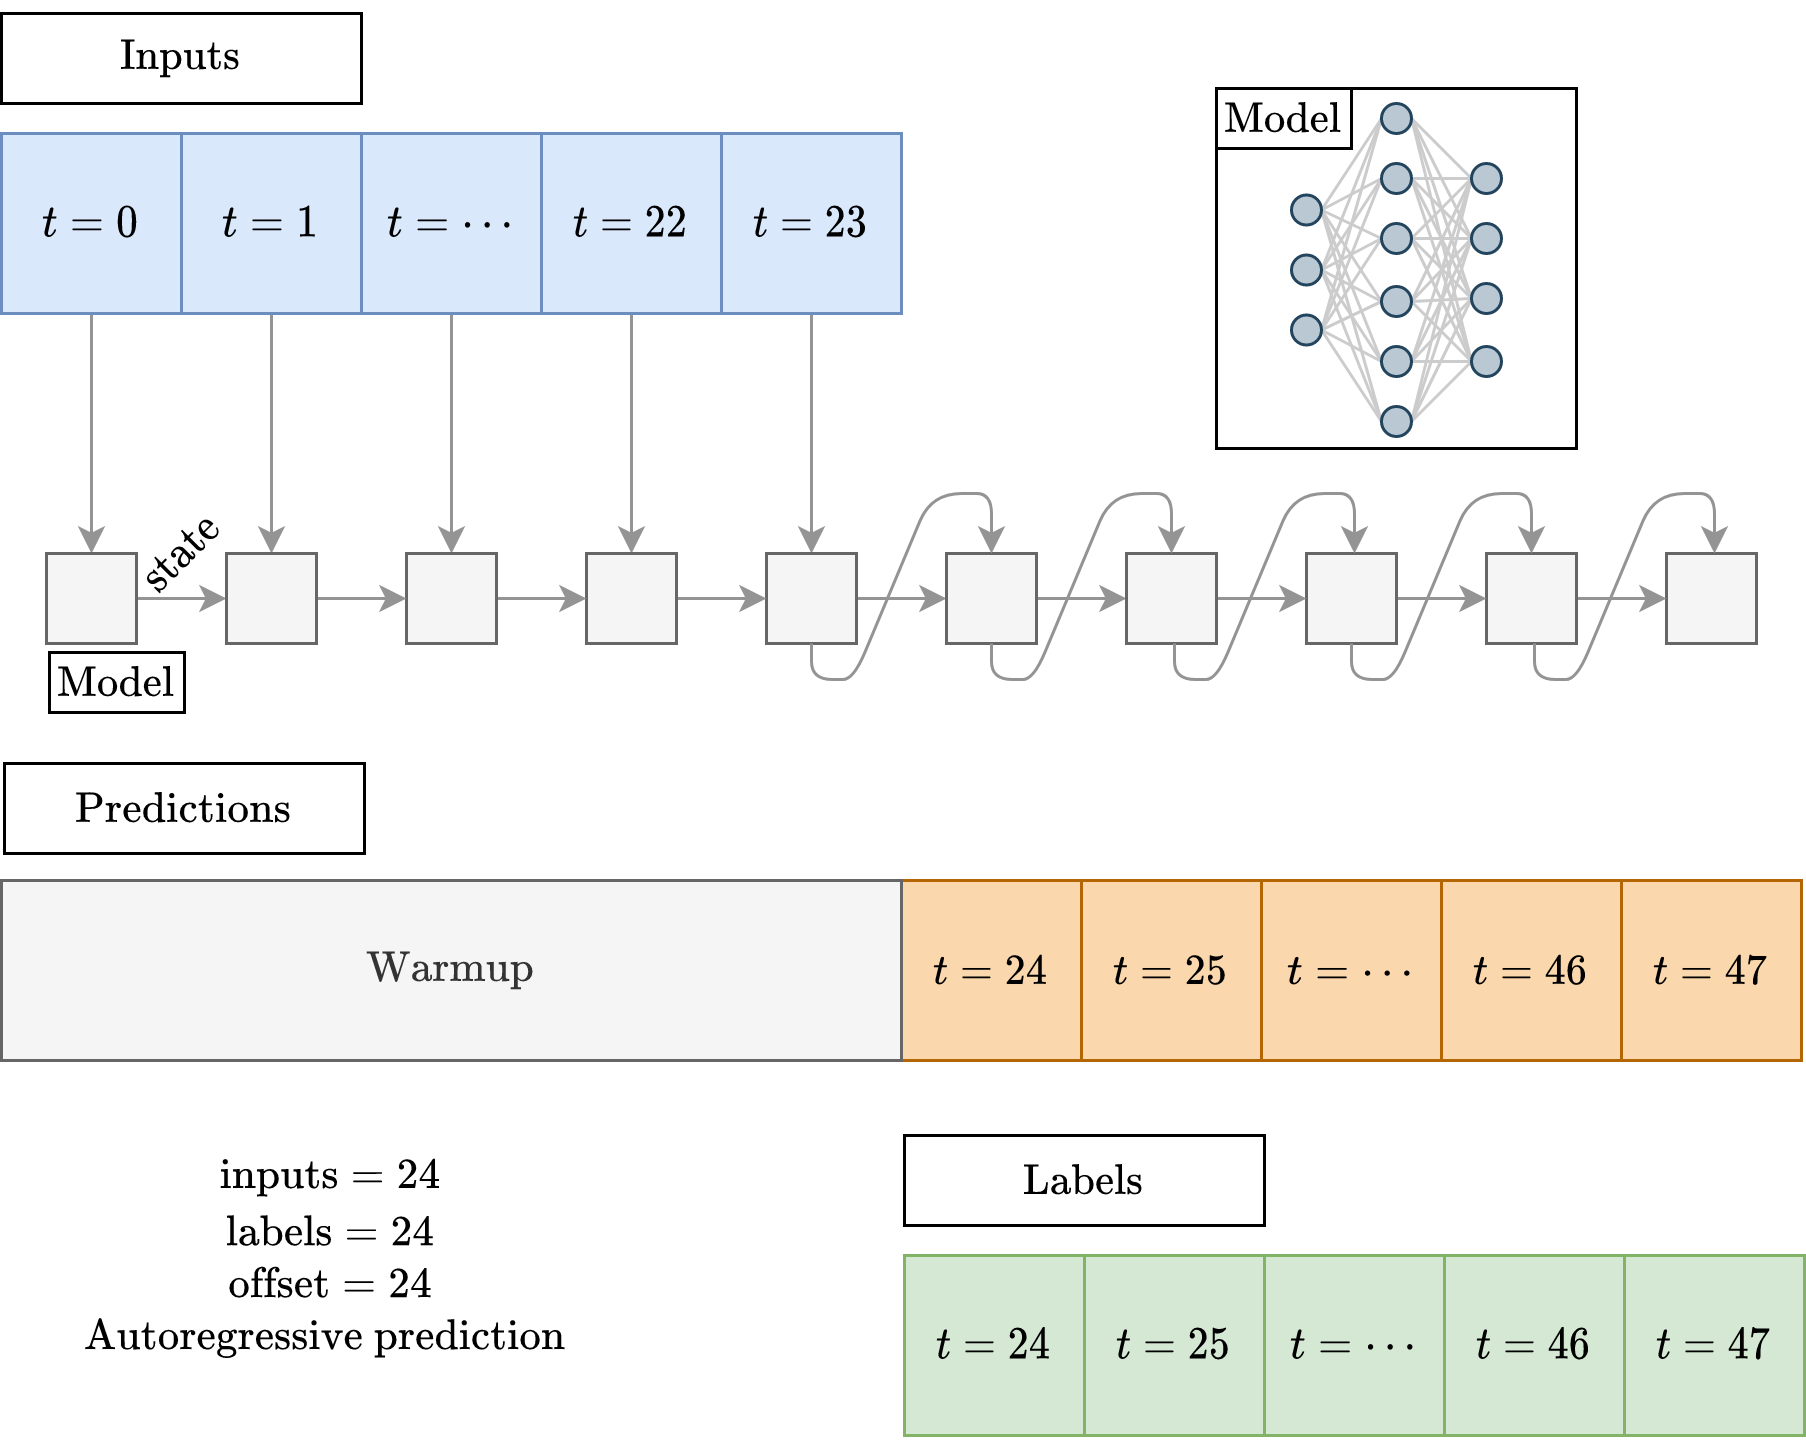
\includegraphics[width=12cm]{images/solution/modules/windows/windows-predictions-ar.png}
    \caption{Predicción auto-regresivas}
    \end{figure}
\end{itemize}

Una vez que se tengan las ventanas, hay que hacer que la ventana se pueda deslizar y de ese modo generar un nuevos vectores que servirán para el entrenamiento. Pongamos por ejemplo, que se dispone de un \textit{dataset} con 7 intervalos. Se quiere entrenar a un modelo que reciba 3 intervalos de entrada y 1 de salida. Por lo que el modelo se entrenará con un lote (\textit{batch}) de tamaño 4. Visto gráficamente, el funcionamiento de una ventana deslizante:

\begin{figure}[H]
    \centering
    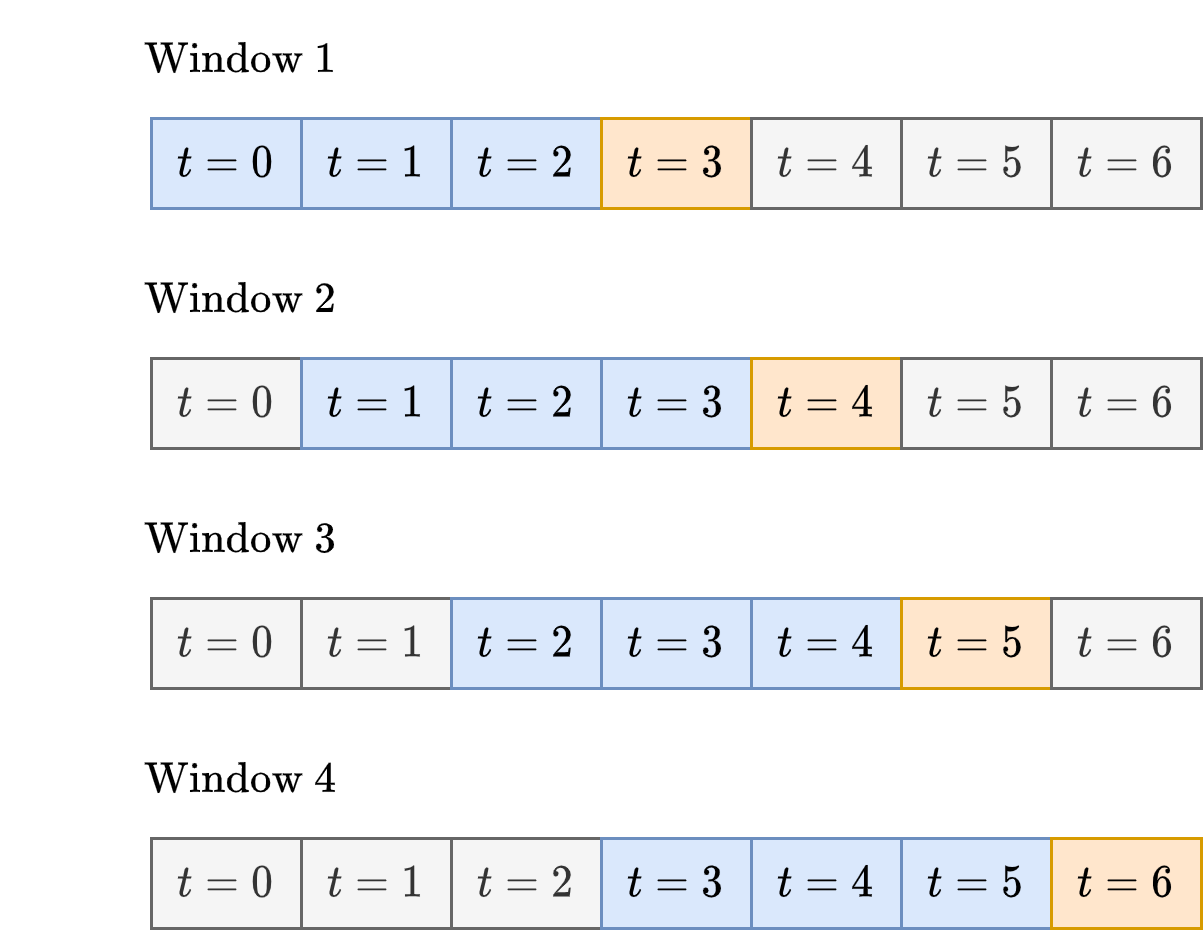
\includegraphics[width=7cm]{images/solution/modules/windows/sliding-windows.png}
    \caption{Funcionamiento de una ventana deslizante.}
\end{figure}


\subsubsection{Código del generador de ventanas}\label{window-generator-code}

Para este módulo se ha generado una clase que se encarga de crear objetos y se basa en gran parte en el tutorial oficial de \textit{Tensorflow} \cite{tensorflow2015-whitepaper} que ha sido modificado para suplir las necesidades del proyecto.
\newline

A continuación se van se explican todas los métodos usadas en la clase por partes.

\begin{itemize}
    \item Índices y \textit{offsets}:  El método \small{\verb|__init__|} (constructor en \textit{Python}) incluye toda la lógica necesaria para los índices de entrada y de etiqueta. También toma los \small{\verb|DataFrames|} de entrenamiento, validación y test como entrada. Estos serán convertidos a \small{\verb|tf.data.Datasets|} de ventanas más tarde. Por último, recibe el índice de la columna donde se encuentra la información temporal. Este índice es un valor igual a $-3$, pues como se puede ver en la tabla \ref{tab:intervals_example}, las tres últimas columnas son las que contienen información sobre la hora, día de la semana y mes.

\begin{minted}[fontsize=\scriptsize]{python}
import tensorflow as tf
import numpy as np


class WindowGenerator():
    def __init__(self, input_width, label_width, shift,
                 train_df, val_df, test_df=None,
                 label_columns_index=-3):

        # Store the datasets
        self.train_df = train_df
        self.val_df = val_df
        self.test_df = test_df

        # Gets the indexes of the label column.
        self.label_columns_index = label_columns_index
        self.label_columns = train_df.columns[:label_columns_index]
                                     .tolist()
        self.label_columns_indices = {name: i for i, name in
                                      enumerate(self.label_columns)}
    
        # Dict of name of column as key and index as value
        self.column_indices = {name: i for i, name in
                               enumerate(train_df.columns)}

        # Work out the window parameters.
        self.input_width = input_width
        self.label_width = label_width
        self.shift = shift
        
        # Handle the indexes and offsets as shown in the diagrams
        # above.
        self.total_window_size = input_width + shift

        self.input_slice = slice(0, input_width)
        self.input_indices = np.arange(self.total_window_size)[
            self.input_slice]

        self.label_start = self.total_window_size - self.label_width
        self.labels_slice = slice(self.label_start, None)
        self.label_indices = np.arange(self.total_window_size)[
            self.labels_slice]
\end{minted}

\item División de la ventana entre \textit{input} y \textit{label}: Dada una lista de intervalos consecutivas, el método \small{\verb|split_window()|} convertirá en una ventana de entradas y una ventana de etiquetas.

\begin{minted}[fontsize=\scriptsize]{python}
def split_window(self, features):
    inputs = features[:, self.input_slice, :]
    labels = features[:, self.labels_slice, :]

    if self.label_columns is not None:
        labels = tf.stack(
            [labels[:, :, self.column_indices[name]]
                for name in self.label_columns],
            axis=-1)

    # Slicing doesn't preserve static shape information, so set
    # the shapes manually. This way the `tf.data.Datasets` are
    # easier to inspect.
    inputs.set_shape([None, self.input_width, None])
    labels.set_shape([None, self.label_width, None])
    return inputs, labels
\end{minted}


\item Creación de los \small{\verb|tf.data.Datasets|}: Finalmente este método small{\verb|make_dataset()|} tomará un \small{\verb|DataFrame|} de intervalos y lo convertirá en un \small{\verb|tf.data.Dataset|} de pares (\small{\verb|input_window|}, \small{\verb|label_window|}). Y como se puede ver a continuación se han creado \textit{batches} de tamaño $32$.


\begin{minted}[fontsize=\scriptsize]{python}
def make_dataset(self, data):
    if data is None:
        print("Data is None")
        return

    data = np.array(data, dtype=np.float32)
    ds = tf.keras.preprocessing.timeseries_dataset_from_array(
        data=data,
        targets=None,
        sequence_length=self.total_window_size,
        sequence_stride=1,
        shuffle=True,
        batch_size=32,)

    ds = ds.map(self.split_window)

    return ds
\end{minted}

\item La clase \small{\verb|WindowGenerator|} contiene los \small{\verb|DataFrame|} de entrenamiento, validación y test. Por lo que al final, se añaden las propiedades para acceder a ellos que son de tipo \small{\verb|tf.data.Datasets|} usando el método anterior \small\verb|make_dataset|:
\begin{minted}[fontsize=\scriptsize]{python}
@property
def train(self):
  return self.make_dataset(self.train_df)

@property
def val(self):
  return self.make_dataset(self.val_df)

@property
def test(self):
  return self.make_dataset(self.test_df)
\end{minted}
\end{itemize}

\newpage
\section{Modelos usados}

En esta sección se explican los modelos que se han desarrollado. Se ha creado un modelo \textit{baseline} y cuatro redes neuronales con cuatro arquitecturas distintas. Los resultados de estos modelos se pueden ver en la Sección \ref{results}.
\newline

\subsection{Modelo base}\label{baseline_model}
Antes de definir las redes neuronales de este trabajo, se ha realizado un estudio de otros trabajos y resultados similares que se puede observar en la sección \ref{similar_projects}. Esto permite poder usar los resultados de otros proyectos como punto de referencia, sabiendo si el desarrollo de esta práctica está mejorando los resultados obtenidos por otros proyectos o no. Además de tener los puntos de referencias de otros proyectos, se ha definido un modelo base.
\newline

Un modelo base es un modelo trivial que se suele desarrollar cuando se quiere resolver un problema de predicción o clasificación para saber si el resto de modelos que se van a desarrollar mejoraran el resultado. En este proyecto, el modelo base desarrollado no tiene lógica y simplemente devuelve el valor que hubo con una semana de anterioridad como predicción.  
\newline

A continuación se puede ver gráficamente las predicciones del modelo respecto a los valores reales:
\begin{figure}[H]
    \centering
    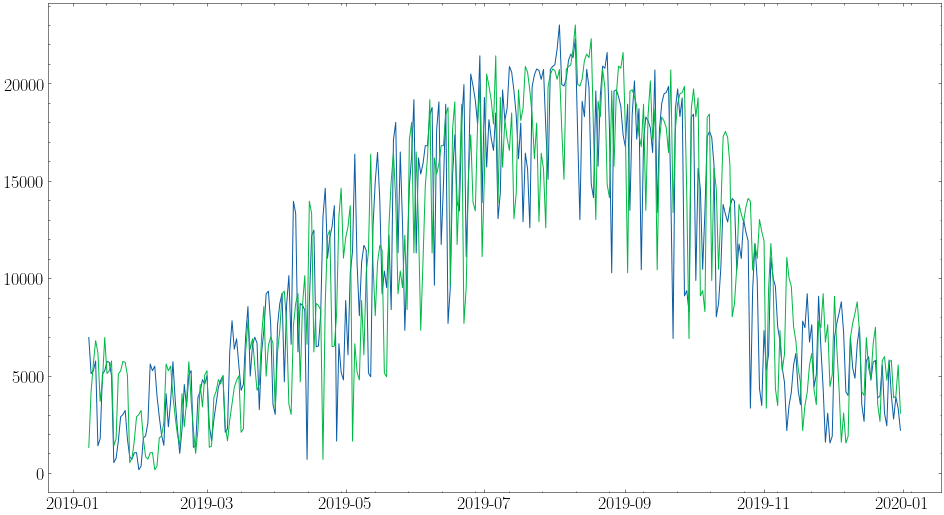
\includegraphics[width=16cm]{images/solution/predictions/baseline-predictions.png}
    \caption{Predicciones del modelo básico}
    \label{fig:baseline-predictions}
\end{figure}

Se puede observar que las predicciones son los mismo valores reales pero desplazados una semana. Una vez desarrollado este modelo, se han calculado las métricas que se muestran en la sección \ref{results} junto con el resto de los resultados de los otros modelos.

\subsection{Modelos con redes neuronales}
\subsubsection{Modelo denso}


Este modelo es un modelo con solo capas de tipo \textit{forward-pass}. Tiene otras dos capas pero que no implementan lógica asociada a lo que es la red neuronal en sí, sino que son capas de traducción de matriz a vector y viceversa como se explicará a continuación. Gráficamente la red que se ha definido es la siguiente:
\begin{figure}[H]
    \centering
    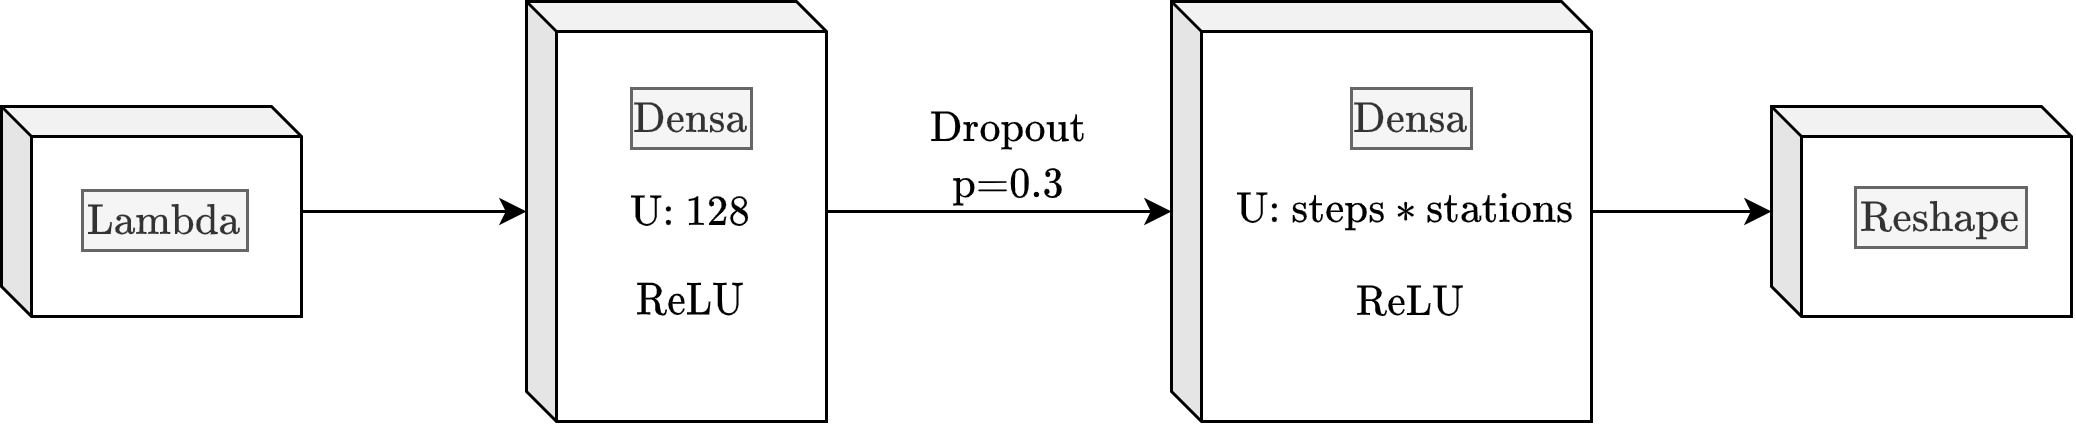
\includegraphics[width=12cm]{images/solution/models/dense.png}
    \caption{Modelo denso}
    \label{fig:dense-model}
\end{figure}

La primera capa oculta tiene 128 unidades. La cantidad de neuronas que tiene una capa oculta es un parámetro que se ha puesto de forma pseudoaleatoria. Se han realizado distintas combinaciones probando distintas cantidades de unidades y 128 es el que mejor resultado a dado. La segunda capa oculta tiene la misma cantidad de unidades que valores tiene que devolver el modelo, que es un valor calculado por la multiplicación entre el número de estaciones con las que se está trabajando, 633, por el número de intervalos que se quieren calcular. Por ejemplo, si se quiere calcular un único intervalo para todas las estaciones, el vector de dicha capa será de $633$ elementos, si se quiere calcular dos intervalos, el número de elementos del vector será $1266 = 2 \times 633$ y así sucesivamente. Esta capa es común a todos los modelos que se explicarán de aquí en adelante.
\newline

La última capa es una capa de tipo \textit{Reshape}. Esta capa no tiene ni función de activación ni parámetros que ajustar porque lo único que hace es ajustar el vector de la capa anterior a una matriz más comprensible y con la que se puede trabajar de forma más cómoda con el dataset. Básicamente, devolverá un vector de vectores, donde cada elemento será un intervalo y cada intervalo tendrá la predicción para cada estación. Siguiendo la misma lógica, la primera capa es de tipo \textit{Lambda} y se encarga de realizar la tarea opuesta, dada una matriz obtener un vector. Las capas \textit{Lambda} son capas en las que el usuario define una función que se quiera ejecutar.
\newline

El código de este modelo se ha definido como se muestra a continuación:

\begin{minted}[fontsize=\scriptsize]{python}
from tensorflow.keras.models import Sequential
from tensorflow.keras.layers import Reshape, Dense, Dropout, Lambda

# `steps` is a variable which has the number of intervals to be predict
steps = 0 

# `stations` is the number of stations in the bike network
stations = 0

dense_model = Sequential([
    # Matrix to vector
    Lambda(lambda x: x[:, -1:, :]), 
    
    # Input layer
    Dense(128, activation="relu"),

    Dropout(0.3),
    
    # Ouput layer
    Dense(steps * stations),
                  
    # Vector to matrix
    Reshape([steps, stations])
])
\end{minted}


Los resultados del modelo se pueden ver junto al resto de resultados en la sección \ref{results}.
\subsubsection{Modelo recurrente básico}

Este modelo es el mismo modelo que el denso pero añadiendo una nueva capa recurrente simple explicada en la sección \ref{rnn_theory}. La capa recurrente simple es una capa que nos permite usar información de otros intervalos anteriores que serán usados para la predicción final. Esta capa recurrente tiene 100 unidades y gráficamente el modelo se puede representar de la siguiente forma:
\begin{figure}[H]
    \centering
    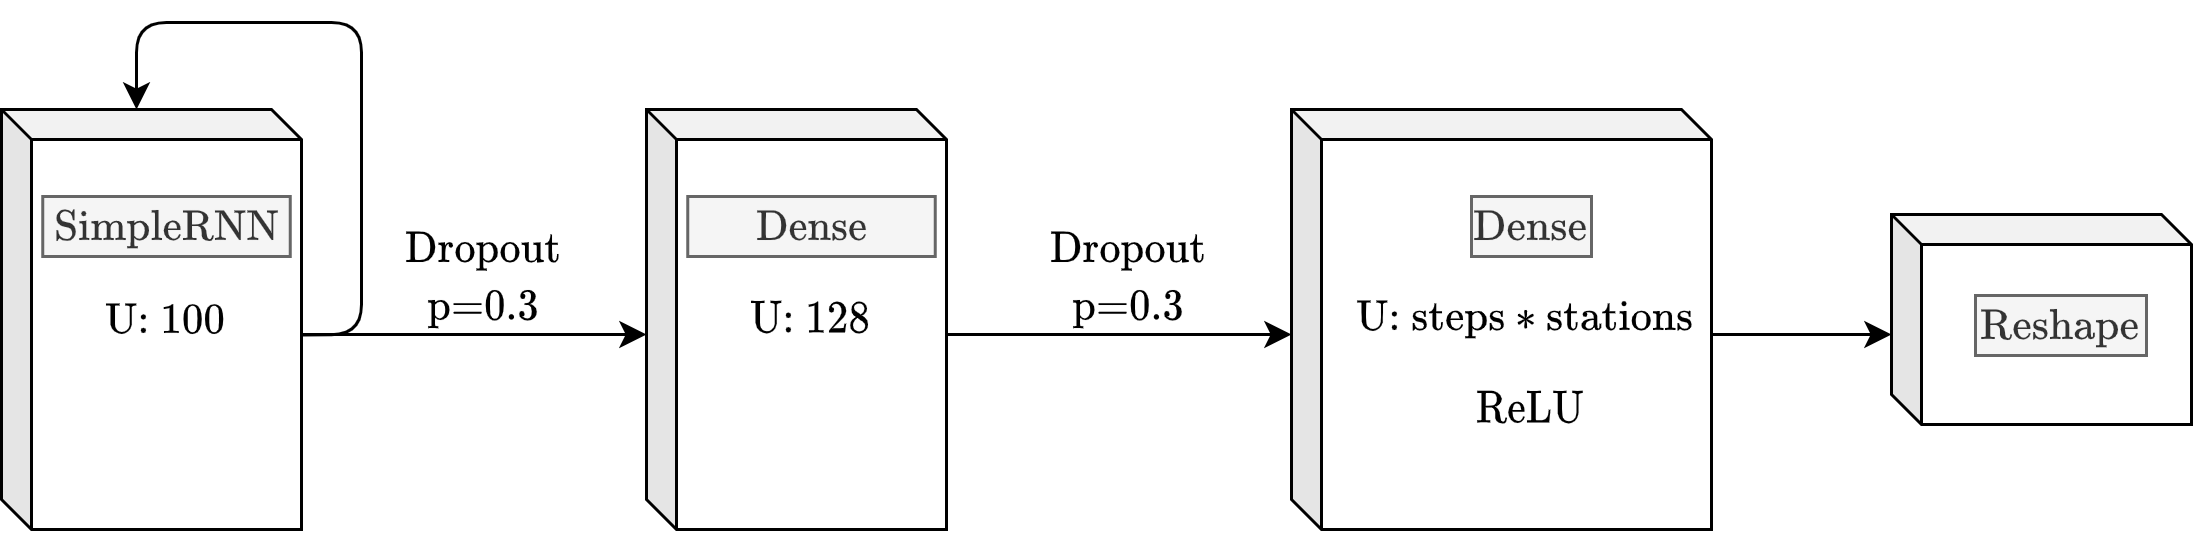
\includegraphics[width=12cm]{images/solution/models/simpleRnn.png}
    \caption{Modelo recurrente básico}
    \label{fig:dense-model}
\end{figure}

Como se puede observar es una extensión del modelo denso explicado en la sección anterior pero añadiendo una nueva capa de tipo \textit{SimpleRNN}. El código de este modelo se ha definido como se muestra a continuación:
\begin{minted}[fontsize=\scriptsize]{python}
from tensorflow.keras.models import Sequential
from tensorflow.keras.layers import Reshape, Dense, Dropout, Lambda, SimpleRNN

# `steps` is a variable which has the number of intervals to be predict
steps = 0 

# `stations` is the number of stations in the bike network
stations = 0

rnn_model = Sequential([
    # Matrix to vector
    Lambda(lambda x: x[:, -1:, :]),
    
    SimpleRNN(100, return_sequences=True),
    
    Dropout(0.3),
    Dense(128),
    Dropout(0.3),
    
    # Ouput layer
    Dense(steps * stations),
    
    # Vector to matrix
    Reshape([steps, stations])
])
\end{minted}


Los resultados del modelo se pueden ver junto al resto de resultados en la sección \ref{results}.
\subsubsection{Modelo recurrente LSTM}

Este modelo es igual que el modelo recurrente básico pero sustituyendo la capa recurrente por una capa LSTM la cual es más compleja y permite que la red aprenda más patrones que están distribuidos en el tiempo como se explicó en la sección \ref{lstm_theory}. Esta capa recurrente tiene 128 unidades y gráficamente el modelo se puede representar de la siguiente forma:
\begin{figure}[H]
    \centering
    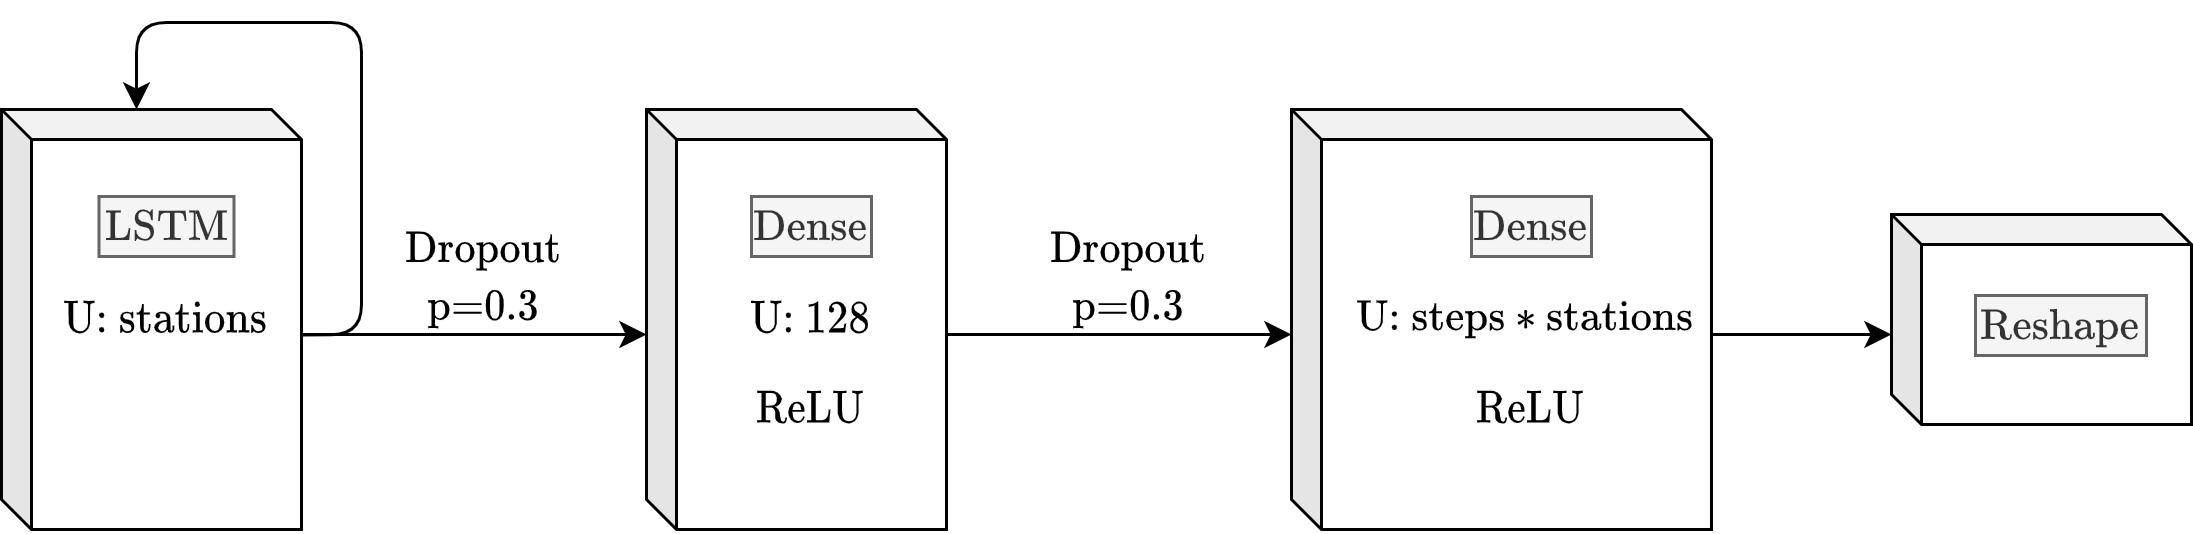
\includegraphics[width=12cm]{images/solution/models/LSTM.png}
    \caption{Modelo recurrente LSTM}
    \label{fig:dense-model}
\end{figure}

Como se puede observar es el mismo modelo pero sustituyendo la capa \textit{SimpleRNN} por una \textit{LSTM}. El código de este modelo se ha definido como se muestra a continuación:
\begin{minted}[fontsize=\scriptsize]{python}
from tensorflow.keras.models import Sequential
from tensorflow.keras.layers import Reshape, Dense, Dropout, Lambda, LSTM

# `steps` is a variable which has the number of intervals to be predict
steps = 0 

# `stations` is the number of stations in the bike network
stations = 0

lstm_model = Sequential([
    # LSTM layer
    LSTM(stations, return_sequences=False),
    
    Dropout(0.3),
    Dense(128, activation="relu"),
    
    # Output layer
    Dropout(0.3),
    Dense(steps * stations, activation="relu"),
    
    # Vector to matrix
    Reshape([steps, stations])
])
\end{minted}

Los resultados del modelo se pueden ver junto al resto de resultados en la sección \ref{results}.
\subsubsection{Modelo autoregresivo (AR)}\label{model_ar}


Un modelo autoregresivo es otro tipo de redes neuronal recurrente. Esta red tiene como peculiaridad que el resultado obtenido se usa como valor de entrada para el calculo de la siguiente iteración. El modelo generado gráficamente es el siguiente:
\begin{figure}[H]
    \centering
    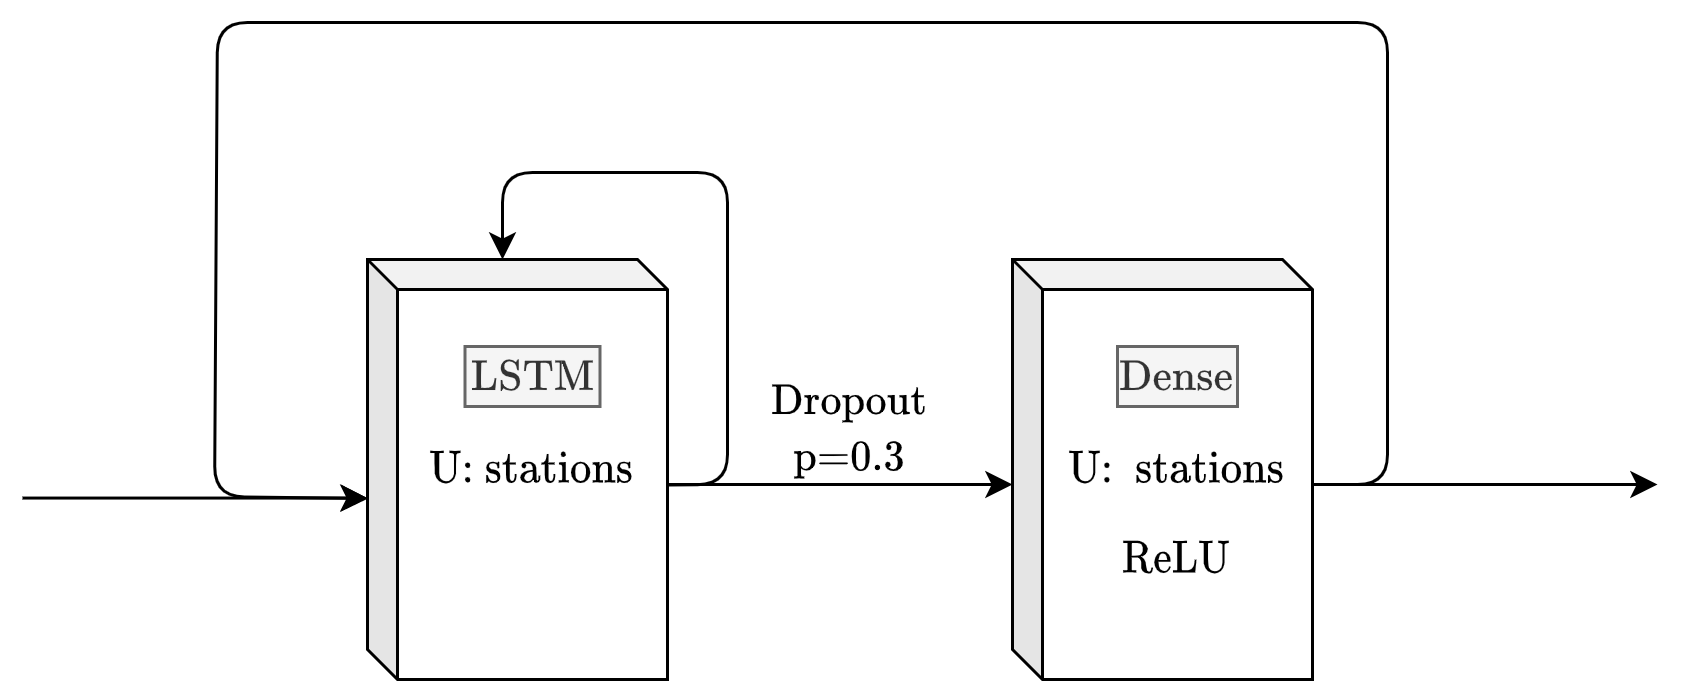
\includegraphics[width=10cm]{images/solution/models/AR.png}
    \caption{Modelo recurrente Autoregresivo}
    \label{fig:dense-model}
\end{figure}

El modelo tiene una capa LSTM junto con una capa densa. La salida de esta capa que es la predicción del modelo se reintroduce en el modelo para predecir el resto de predicciones.
\newline

\textit{Tensorflow} no dispone de un modelo en su librería que supliese las necesidades que buscábamos, por esa razón, se ha tenido que implementar este modelo usando otra técnica. Se ha creado una clase nueva que hereda de \small\verb|tf.keras.Model| y la cual tiene tres métodos: \small\verb|__init__|, \small\verb|warmup| y \small\verb|call|. De esta forma se pueden generar modelos que puedan tener arquitecturas singulares y distintas a las \textit{pass-forward}. Para la implementación se ha seguido la documentación de \textit{Tensorflow} \cite{tensorflow2015-whitepaper} y \textit{Keras} \cite{keras}.
\newline

La clase usada para definir el modelo autoregresivo ha sido el siguiente:
\begin{minted}[fontsize=\scriptsize]{python}
import tensorflow as tf
from tensorflow.keras.layers import LSTMCell, RNN, Dense

class AutoRegressive(tf.keras.Model):
    def __init__(self, lstm_units, steps, stations):
        super().__init__()
        self.steps = steps
        self.stations = stations
        self.lstm_units = lstm_units
        
        # First LSTM layer
        self.lstm_cell = LSTMCell(lstm_units)
        # Also wrap the LSTMCell in an RNN to simplify the `warmup` method.
        self.lstm_rnn = RNN(self.lstm_cell, return_state=True)
        
        # Ouput layer
        self.dense = Dense(stations, activation="relu")

    def warmup(self, inputs):
        # inputs.shape => (batch, time, features)
        # x.shape => (batch, lstm_units)
        x, *state = self.lstm_rnn(inputs)

        # predictions.shape => (batch, features)
        prediction = self.dense(x)
        return prediction, state

    def call(self, inputs, training=None):
        # Use a TensorArray to capture dynamically unrolled outputs.
        predictions = []

        # Initialize the lstm state
        prediction, state = self.warmup(inputs)

        # Insert the first prediction
        predictions.append(prediction)

        # Run the rest of the prediction steps
        for n in range(1, self.steps):
            # Use the last prediction as input.
            x = prediction
            
            # Concat with timestamp variables
            x = tf.concat([x, inputs[:,-1,-3:]], 1)
            
            # Execute one lstm step.
            x, state = self.lstm_cell(x, states=state, training=training)
                                      
            # Convert the lstm output to a prediction.
            prediction = self.dense(x)
            
            # Add the prediction to the output
            predictions.append(prediction)

        # predictions.shape => (time, batch, features)
        predictions = tf.stack(predictions)
        
        # predictions.shape => (batch, time, features)
        predictions = tf.transpose(predictions, [1, 0, 2])
        
        return predictions
\end{minted}


Para crear un nuevo modelo simplemente se genera una nueva instancia de la siguiente manera:
\begin{minted}[fontsize=\scriptsize]{python}
AutoRegressive(lstm_units=stations, steps=steps, stations=stations)
\end{minted}

Los resultados del modelo se pueden ver junto al resto de resultados en la sección \ref{results}.
\subsection{Ventanas}

Como se ha explicado en la sección \ref{window-generator}, se pueden generar predicciones en función de los argumentos de entrada. Es decir, se puede crear un modelo que dado una cantidad $X$ de intervalos, pueda predecir una cantidad $Y$ de intervalos. Se quería comparar diferentes ajustes que se pueden realizar a las ventanas y ver los resultados obtenidos. En definitiva, se ha creado un modelo distinto para cada uno de los tamaños de ventana.
\newline

De aquí en adelante, se hará referencia a las configuración de ventana con tuplas, donde el primer término es el tamaño de intervalos de entrada y el segundo elemento el tamaño de intervalos que el modelo predice. Por ejemplo dada la siguiente tupla 12-5, quiere decir que el modelo desarrollado usa una ventana con 12 intervalos de entrada y 5 intervalos de salida.
\newline

En total se han usado 15 configuraciones de ventana distintas: 3-1, 5-1, 8-1, 8-3, 8-5, 12-1, 12-3, 12-5, 24-1, 24-3, 24-5, 36-8, 36-12, 48-12, 48-24. Como se han desarrollado 4 arquitecturas de neuronales diferentes, al final se han desarrollado 60 modelos más el modelo básico. 

\subsection{Entrenamiento, validación y test de las redes neuronales}


Una vez creado los modelos, se ha codificado una función para automatizar el proceso de entrenamiento, validación y test de cada uno de los modelos y de además de obtener las métricas que se necesitarán para poder estudiar y comparar los distintos modelos. El código es el siguiente:

\begin{minted}[fontsize=\scriptsize]{python}

MAX_EPOCHS = 150

'''
Compiles and train model

@param model which will be training
@param window with the Datasets used
@param max_epoch for training
@param should_stop if detects overfitting the stops with a patience of 10
@param lr (learning rate) of the model
'''
def compile_and_fit(model, window, max_epochs=MAX_EPOCHS, should_stop=False, lr=0.001):
    model.compile(
        loss=tf.losses.Huber(),
        optimizer=tf.optimizers.Adam(lr=lr),
        metrics=[MeanSquaredLogarithmicError(), MeanSquaredError(), MeanAbsoluteError(),
                RootMeanSquaredError(), RootMeanSquaredLogarithmicError])
    
    # Define the callbacks for the training proccess
    # PlotLossesKeras plots training and validation for every epoch in real time
    # early_stopping allows to stop if detects overfitting
    cbs = [PlotLossesKeras()] + ([EarlyStopping(monitor='val_loss',
                                                      patience=10,
                                                      mode='min')] if should_stop else [])
    
    model.fit(window.train, epochs=max_epochs,
                        validation_data=window.val,
                        callbacks=cbs,
                        verbose=2)
    
'''
Computes metrics and returns it as DataFrame
'''
def get_metrics(model, window):
    train_metrics = model.evaluate(window.train)
    val_metrics = model.evaluate(window.val)
    test_metrics = model.evaluate(window.test)

    metrics_names = model.metrics_names
    metrics_names[0] = "huber"
    metrics = pd.DataFrame({
        "names": metrics_names,
        "train": train_metrics,
        "val": val_metrics,
        "test": test_metrics,
    })

    return metrics


windows_sizes=[(3, 1), (5, 1), (8, 1), (8, 3), (8, 5), (12, 1), 
                (12, 3), (12, 5), (24, 1), (24, 3), (24, 5)]

'''
Given a model it will train with different windows sizes

@param model which will be training
@param max_epoch for training
@param lr (learning rate) of the model
@param windows_sizes a list of tuples containing window sizes as (input, output)
'''
def model_generator(model, lr, max_epochs=150, windows_sizes=windows_sizes):
    # Loads and splits the DataFrames
    df = load_dataset()
    train_df, val_df, test_df = split_dataset(df)
    
    # For every windo
    for w in windows_sizes:
        # Create the windoe
        input_width, steps = r
        window = WindowGenerator(input_width=input_width,
                                 label_width=steps,
                                 shift=steps,
                                 train_df=train_df,
                                 val_df=val_df,
                                 test_df=test_df)

        
        # Train model
        compile_and_fit(
            model, window, lr=lr, should_stop=True, max_epochs=max_epochs)
        
        # Save metrics
        metrics = get_metrics(model, window)
        filename = "/path/to/results/{model.get_name()}" + \
                    "-{input_width}-{steps}.csv"
        metrics.to_csv(filename)
\end{minted}


Como se puede ver en el código, dado un modelo, la función se encarga de entrenar dicho modelo pero con distintas configuraciones de ventana y posteriormente guarda las métricas en un CSV. 
\newpage
\section{Resultados}\label{results}

En esta sección se mostrarán todos los resultados obtenidos con los diferentes modelos. En total se han desarrollado 4 modelos (1 modelo básico y 3 redes neuronales). Estos modelos se han ido iterando desde un modelo básico hasta modelos más complejos. Dicho proceso de mejora se ve reflejado en las métricas obtenidas.

\subsection{Métricas usadas}
En total se han usado 6 métricas distintas para medir el rendimiento de los modelos. Además, uno de esas métricas, la pérdida de Huber (ver sección \ref{huber_loss}) se ha usado además como función de coste.

\subsubsection{Pérdida de Huber}

Como se explica en la Sección \ref{huber_loss}, está función de pérdida no prioriza los datos atípicos sino que trata a todos los datos de forma similar. Esto es muy útil, para el problema que queremos resolver.

En el dataset que estamos usando, un dato que no siga el patrón (\textit{outlier}) no significa que sea un error que se deba de tener en cuenta como puede ocurrir en otros tipos de problemas. Por ejemplo, en una estación de bicicletas justo en frente de una facultad recibe una gran demanda un jueves a las 17 mientras que el resto de jueves no ha tenido tanta demanda para dicho intervalo. Esto se debe a un acontecimiento único, por ejemplo un examen en dicha facultad para ese día. Este dato, al ser un dato válido y no un error como tal, la red no aprenderá de inmediato que los jueves habrá dicha demanda sino que harán faltas múltiples días en los que se repita para que la red comience a ajustarse a dichos datos y por eso la pérdida de Huber se adapta bien a este tipo de problema. La ecuación de la pérdida de Huber es la siguiente:

\begin{equation}
\centering
    \begin{split}
    \text{Huber} = \left\{ 
        \begin{array}{cl} 
            MSE & \text{si }|\hat{y}-y| \le \delta, \\
            MAE & \text{e.o.c.}
        \end{array}\right.
    \end{split}
\end{equation}

Para la implementación del código se ha usado la propia implementación de la librería de \textit{Keras}:

\begin{minted}{python}
from tf.losses import Huber
\end{minted}

\subsubsection{MAE}

El error absoluto medio (MAE) es una de las métricas más básicas y rápidas de calcular. Se calcula usando la media entre las diferencias entre los valores reales y los valores predichos como se puede ver a continuación:

\begin{equation}
\centering
    \begin{split}
        \text{MAE} = \frac{1}{n} \sum_{i=1}^n |y_i - \hat{y_i}|
    \end{split}
\end{equation}

Para hacer uso de esta ecuación en \textit{Keras}, se puede importar de la siguiente forma:


\begin{minted}{python}
from tf.metrics import MeanAbsoluteError
\end{minted}

\subsubsection{MSE y RMSE}

Estas dos métricas indican básicamente los mismo. El MSE es un valor que se obtiene al calcular la media entre todos los valores obtenidos al aplicar el cuadrado a la diferencia entre el valor real y el valor predicho como se puede ver a continuación:

\begin{equation}
\centering
    \begin{split}
        \text{MSE} = \frac{1}{n} \sum_{i=1}^n (\hat{y_i} - y_i)^2
    \end{split}
\end{equation}

Por otro lado, RMSE es la raíz cuadrada del RMSE como se puede observar a continuación:

\begin{equation}
\centering
    \begin{split}
        \text{RMSE} = \sqrt{MSE}
    \end{split}
\end{equation}

Para poder hacer cálculo de MSE y RMSE se pueden importar desde \textit{tensorflow}.

\begin{minted}{python}
from tf.losses import MeanSquaredError
from tf.metrics import RootMeanSquaredError
\end{minted}

\subsubsection{MSLE y RMSLE}

Esta métrica se usa porque hay multitud de proyectos, entre ellos, la competición de \textit{Kaggle} (ver sección \ref{kaggle_competition}) que usan estas métricas y de esa forma poder comparar los resultados. La explicación del MSLE se puede ver en la sección \ref{MSLE_loss}. RMSLE es igual que MSLE pero aplicándole una raíz cuadrada:

\begin{equation}
\centering
    \begin{split}
        \text{MSLE} &= \frac{1}{n} \sum_{i=1}^n \left(\log{\left(\frac{y_i + 1}{\hat{y_i} + 1}\right)}\right)^2 \\
        \text{RMSLE} &= \sqrt{MSLE}
    \end{split}
\end{equation}

Para poder hacer cálculo de MSLE se puede importar la función de \textit{Keras}. Esta función además nos sirve para poder definir la función RMSLE como se muestra a continuación:

\begin{minted}{python}
from tf.keras.losses import MeanSquaredLogarithmicError
def RootMeanSquaredLogarithmicError(y_true, y_pred):
    msle = MeanSquaredLogarithmicError(y_true, y_pred)
    return tf.keras.backend.sqrt(msle)
\end{minted}


\subsection{Modelo básico}
El modelo básico como se ha explicado en la sección \ref{baseline_model}, devuelve la cantidad de bicicletas que se iniciaron para un intervalo la anterior semana a la cual se quiere predecir el dato. Calculando todas las métricas, los resultados de este modelo son son los siguientes:

\begin{table}[H]
    \centering
    \begin{tabular}{l|rr}
    \toprule
    Métricas &      val &      test \\
    \midrule
    MSLE &  0.221549 &  0.239364 \\
    MSE &  3.383871 &  3.699979 \\
    MAE &  0.603720 &  0.647458 \\
    HUBER &  0.462739 &  0.499985 \\
    RMSE &  1.913998 &  1.914635 \\
    RMSLE &  0.470690 &  0.489248 \\
    \bottomrule
    \end{tabular}
    \caption{Métricas obtenidas del modelo básico.}
\end{table}

Estos valores son los que se usarán como referencia para poder comparar los modelos que se desarrollen y comprobar que se está consiguiendo una mejora.



\subsection{Redes neuronales}

A continuación se muestran los resultados de todos los modelos que se han entrenado para estudiar como se comporta en función del tamaño de la ventana deslizante. Todos los modelos tienen los mismo hyperparámetros que se han explicado en la sección \ref{models}. A continuación se puede ver una tabla con todos los resultados obtenidos. Las columnas representan los modelos usados, los cuales todos tienen las métricas obtenidas tanto para el \textit{dataset} de \textit{validation} como el \textit{dataset} de \textit{testing}. Las filas están dividas tanto por las métricas usadas como por el tamaño de ventana para cada modelo. En total se han desarrollado 44 modelos (11 tamaños de ventanas distinos por 4 modelos de redes neuronales):


\begin{longtable}{ll|rr|rr|rr|rr}
\toprule
      &          & \multicolumn{2}{l}{Dense} & \multicolumn{2}{l}{RNN} & \multicolumn{2}{l}{LSTM} & \multicolumn{2}{l}{AR} \\
      &          & val & test & val & test & val & test & val\_ar & test\_ar \\
\midrule
\multirow{15}{*}{HUBER} & (3, 1) &     0.344 &      0.380 &   0.334 &    0.374 &    0.474 &     0.508 &  0.290 &   0.321 \\
      & (5, 1) &     0.375 &      0.411 &   0.347 &    0.388 &    0.476 &     0.510 &  0.296 &   0.330 \\
      & (8, 1) &     0.410 &      0.445 &   0.352 &    0.389 &    0.477 &     0.512 &  0.291 &   0.324 \\
      & (8, 3) &     0.348 &      0.380 &   0.331 &    0.369 &    0.293 &     0.329 &  0.295 &   0.331 \\
      & (8, 5) &     0.373 &      0.411 &   0.346 &    0.385 &    0.301 &     0.342 &  0.303 &   0.342 \\
      & (12, 1) &     0.435 &      0.472 &   0.378 &    0.418 &    0.472 &     0.506 &  0.288 &   0.320 \\
      & (12, 3) &     0.344 &      0.379 &   0.334 &    0.370 &    0.294 &     0.330 &  0.302 &   0.338 \\
      & (12, 5) &     0.371 &      0.409 &   0.346 &    0.386 &    0.303 &     0.340 &  0.307 &   0.344 \\
      & (24, 1) &     0.460 &      0.495 &   0.434 &    0.474 &    0.472 &     0.507 &  0.290 &   0.323 \\
      & (24, 3) &     0.353 &      0.386 &   0.332 &    0.370 &    0.295 &     0.331 &  0.300 &   0.335 \\
      & (24, 5) &     0.363 &      0.401 &   0.347 &    0.386 &    0.301 &     0.341 &  0.311 &   0.348 \\
      & (36, 8) &     0.355 &      0.399 &   0.358 &    0.397 &    0.299 &     0.338 &  0.317 &   0.358 \\
      & (36, 12) &     0.362 &      0.403 &   0.373 &    0.409 &    0.306 &     0.348 &  0.335 &   0.385 \\
      & (48, 12) &     0.367 &      0.408 &   0.370 &    0.409 &    0.306 &     0.347 &  0.327 &   0.369 \\
      & (48, 24) &     0.374 &      0.414 &   0.385 &    0.423 &    0.311 &     0.353 &  0.337 &   0.374 \\
\hline \multirow{15}{*}{MSLE}  & (3, 1) &     0.136 &      0.154 &   0.130 &    0.149 &    0.235 &     0.253 &  0.115 &   0.131 \\
      & (5, 1) &     0.153 &      0.171 &   0.140 &    0.160 &    0.240 &     0.258 &  0.117 &   0.134 \\
      & (8, 1) &     0.177 &      0.195 &   0.143 &    0.162 &    0.242 &     0.261 &  0.115 &   0.131 \\
      & (8, 3) &     0.134 &      0.151 &   0.129 &    0.148 &    0.114 &     0.131 &  0.118 &   0.135 \\
      & (8, 5) &     0.149 &      0.170 &   0.136 &    0.156 &    0.117 &     0.135 &  0.123 &   0.142 \\
      & (12, 1) &     0.198 &      0.217 &   0.157 &    0.177 &    0.233 &     0.251 &  0.117 &   0.132 \\
      & (12, 3) &     0.132 &      0.150 &   0.129 &    0.147 &    0.114 &     0.131 &  0.123 &   0.140 \\
      & (12, 5) &     0.148 &      0.169 &   0.136 &    0.157 &    0.118 &     0.135 &  0.124 &   0.142 \\
      & (24, 1) &     0.217 &      0.235 &   0.194 &    0.217 &    0.234 &     0.252 &  0.118 &   0.134 \\
      & (24, 3) &     0.137 &      0.154 &   0.130 &    0.149 &    0.115 &     0.132 &  0.122 &   0.139 \\
      & (24, 5) &     0.144 &      0.164 &   0.138 &    0.157 &    0.117 &     0.136 &  0.129 &   0.148 \\
      & (36, 8) &     0.144 &      0.167 &   0.142 &    0.163 &    0.119 &     0.138 &  0.128 &   0.148 \\
      & (36, 12) &     0.148 &      0.169 &   0.148 &    0.166 &    0.121 &     0.141 &  0.138 &   0.162 \\
      & (48, 12) &     0.150 &      0.172 &   0.150 &    0.170 &    0.121 &     0.141 &  0.135 &   0.156 \\
      & (48, 24) &     0.154 &      0.175 &   0.155 &    0.175 &    0.122 &     0.142 &  0.139 &   0.158 \\
\hline 
\multirow{15}{*}{MSE} & (3, 1) &     2.518 &      2.802 &   2.513 &    2.831 &    4.958 &     5.302 &  1.623 &   1.793 \\
      & (5, 1) &     3.228 &      3.526 &   2.678 &    3.022 &    5.017 &     5.375 &  1.684 &   1.899 \\
      & (8, 1) &     3.885 &      4.144 &   2.755 &    3.018 &    5.028 &     5.392 &  1.622 &   1.826 \\
      & (8, 3) &     2.792 &      3.012 &   2.454 &    2.736 &    1.740 &     2.025 &  1.692 &   1.976 \\
      & (8, 5) &     3.185 &      3.550 &   2.730 &    3.031 &    1.890 &     2.284 &  1.839 &   2.155 \\
      & (12, 1) &     4.278 &      4.593 &   3.237 &    3.514 &    5.017 &     5.358 &  1.582 &   1.785 \\
      & (12, 3) &     2.746 &      3.017 &   2.557 &    2.830 &    1.784 &     2.081 &  1.810 &   2.052 \\
      & (12, 5) &     3.171 &      3.510 &   2.692 &    2.998 &    1.929 &     2.240 &  1.895 &   2.187 \\
      & (24, 1) &     4.653 &      4.974 &   4.393 &    4.749 &    5.032 &     5.389 &  1.604 &   1.818 \\
      & (24, 3) &     2.831 &      3.069 &   2.448 &    2.724 &    1.751 &     2.038 &  1.749 &   2.002 \\
      & (24, 5) &     2.990 &      3.330 &   2.701 &    2.980 &    1.872 &     2.222 &  2.122 &   2.403 \\
      & (36, 8) &     2.724 &      3.146 &   2.928 &    3.220 &    1.743 &     2.111 &  2.014 &   2.404 \\
      & (36, 12) &     2.880 &      3.225 &   3.210 &    3.475 &    1.870 &     2.272 &  2.327 &   2.842 \\
      & (48, 12) &     2.965 &      3.333 &   3.098 &    3.372 &    1.855 &     2.246 &  2.093 &   2.476 \\
      & (48, 24) &     3.081 &      3.431 &   3.377 &    3.653 &    1.950 &     2.350 &  2.357 &   2.649 \\
\hline \multirow{15}{*}{MAE} & (3, 1) &     0.508 &      0.550 &   0.519 &    0.565 &    0.699 &     0.738 &  0.468 &   0.504 \\
      & (5, 1) &     0.546 &      0.587 &   0.543 &    0.592 &    0.674 &     0.713 &  0.475 &   0.515 \\
      & (8, 1) &     0.594 &      0.636 &   0.542 &    0.586 &    0.672 &     0.711 &  0.469 &   0.508 \\
      & (8, 3) &     0.524 &      0.563 &   0.521 &    0.565 &    0.469 &     0.512 &  0.455 &   0.498 \\
      & (8, 5) &     0.546 &      0.591 &   0.535 &    0.581 &    0.477 &     0.524 &  0.461 &   0.506 \\
      & (12, 1) &     0.642 &      0.685 &   0.561 &    0.609 &    0.702 &     0.741 &  0.444 &   0.481 \\
      & (12, 3) &     0.519 &      0.560 &   0.520 &    0.562 &    0.469 &     0.512 &  0.458 &   0.501 \\
      & (12, 5) &     0.545 &      0.590 &   0.537 &    0.583 &    0.478 &     0.522 &  0.463 &   0.506 \\
      & (24, 1) &     0.677 &      0.718 &   0.629 &    0.674 &    0.704 &     0.743 &  0.446 &   0.485 \\
      & (24, 3) &     0.526 &      0.564 &   0.522 &    0.567 &    0.473 &     0.515 &  0.453 &   0.494 \\
      & (24, 5) &     0.536 &      0.580 &   0.539 &    0.585 &    0.477 &     0.523 &  0.467 &   0.511 \\
      & (36, 8) &     0.548 &      0.599 &   0.551 &    0.598 &    0.477 &     0.523 &  0.475 &   0.523 \\
      & (36, 12) &     0.556 &      0.604 &   0.562 &    0.606 &    0.485 &     0.534 &  0.488 &   0.545 \\
      & (48, 12) &     0.559 &      0.608 &   0.571 &    0.617 &    0.485 &     0.533 &  0.479 &   0.530 \\
      & (48, 24) &     0.570 &      0.618 &   0.582 &    0.626 &    0.491 &     0.539 &  0.490 &   0.534 \\
\hline \multirow{15}{*}{RMSE} & (3, 1) &     1.587 &      1.674 &   1.585 &    1.683 &    2.225 &     2.303 &  1.273 &   1.339 \\
      & (5, 1) &     1.797 &      1.877 &   1.637 &    1.739 &    2.241 &     2.319 &  1.297 &   1.378 \\
      & (8, 1) &     1.972 &      2.037 &   1.660 &    1.738 &    2.244 &     2.322 &  1.274 &   1.351 \\
      & (8, 3) &     1.671 &      1.735 &   1.567 &    1.655 &    1.318 &     1.424 &  1.301 &   1.406 \\
      & (8, 5) &     1.785 &      1.885 &   1.653 &    1.740 &    1.375 &     1.511 &  1.356 &   1.468 \\
      & (12, 1) &     2.070 &      2.143 &   1.796 &    1.876 &    2.238 &     2.317 &  1.258 &   1.337 \\
      & (12, 3) &     1.659 &      1.738 &   1.598 &    1.679 &    1.336 &     1.441 &  1.346 &   1.434 \\
      & (12, 5) &     1.782 &      1.876 &   1.642 &    1.732 &    1.389 &     1.497 &  1.377 &   1.478 \\
      & (24, 1) &     2.157 &      2.230 &   2.096 &    2.179 &    2.243 &     2.321 &  1.266 &   1.348 \\
      & (24, 3) &     1.682 &      1.752 &   1.565 &    1.651 &    1.323 &     1.428 &  1.323 &   1.415 \\
      & (24, 5) &     1.729 &      1.825 &   1.643 &    1.726 &    1.368 &     1.491 &  1.457 &   1.550 \\
      & (36, 8) &     1.649 &      1.772 &   1.712 &    1.795 &    1.320 &     1.453 &  1.419 &   1.550 \\
      & (36, 12) &     1.697 &      1.798 &   1.792 &    1.865 &    1.366 &     1.508 &  1.526 &   1.685 \\
      & (48, 12) &     1.722 &      1.826 &   1.760 &    1.836 &    1.362 &     1.499 &  1.447 &   1.574 \\
      & (48, 24) &     1.755 &      1.853 &   1.837 &    1.911 &    1.397 &     1.533 &  1.535 &   1.627 \\
\hline \multirow{15}{*}{RMSLE} & (3, 1) &     0.367 &      0.391 &   0.360 &    0.385 &    0.484 &     0.501 &  0.339 &   0.360 \\
      & (5, 1) &     0.390 &      0.413 &   0.373 &    0.399 &    0.488 &     0.506 &  0.342 &   0.365 \\
      & (8, 1) &     0.420 &      0.440 &   0.377 &    0.401 &    0.490 &     0.509 &  0.339 &   0.361 \\
      & (8, 3) &     0.365 &      0.388 &   0.359 &    0.384 &    0.337 &     0.362 &  0.343 &   0.367 \\
      & (8, 5) &     0.385 &      0.411 &   0.368 &    0.394 &    0.341 &     0.367 &  0.350 &   0.376 \\
      & (12, 1) &     0.444 &      0.465 &   0.395 &    0.420 &    0.481 &     0.500 &  0.341 &   0.363 \\
      & (12, 3) &     0.362 &      0.387 &   0.358 &    0.383 &    0.337 &     0.361 &  0.350 &   0.374 \\
      & (12, 5) &     0.384 &      0.410 &   0.369 &    0.395 &    0.342 &     0.367 &  0.351 &   0.376 \\
      & (24, 1) &     0.464 &      0.484 &   0.439 &    0.464 &    0.482 &     0.501 &  0.343 &   0.366 \\
      & (24, 3) &     0.369 &      0.392 &   0.360 &    0.385 &    0.339 &     0.363 &  0.349 &   0.372 \\
      & (24, 5) &     0.378 &      0.404 &   0.370 &    0.396 &    0.342 &     0.368 &  0.359 &   0.384 \\
      & (36, 8) &     0.379 &      0.408 &   0.377 &    0.403 &    0.344 &     0.370 &  0.357 &   0.385 \\
      & (36, 12) &     0.384 &      0.411 &   0.384 &    0.407 &    0.347 &     0.375 &  0.371 &   0.402 \\
      & (48, 12) &     0.387 &      0.414 &   0.387 &    0.412 &    0.347 &     0.375 &  0.367 &   0.395 \\
      & (48, 24) &     0.392 &      0.418 &   0.394 &    0.418 &    0.350 &     0.377 &  0.372 &   0.397 \\
\bottomrule
\end{longtable}

También se han desarrollado gráficas para poder visualizar las métricas más fácilmente usando usando el dataset de \textit{testing}. En todas las gráficas hay una línea horizontal que representa la métrica obtenida por el modelo base:



\begin{figure}[H]
    \centering
    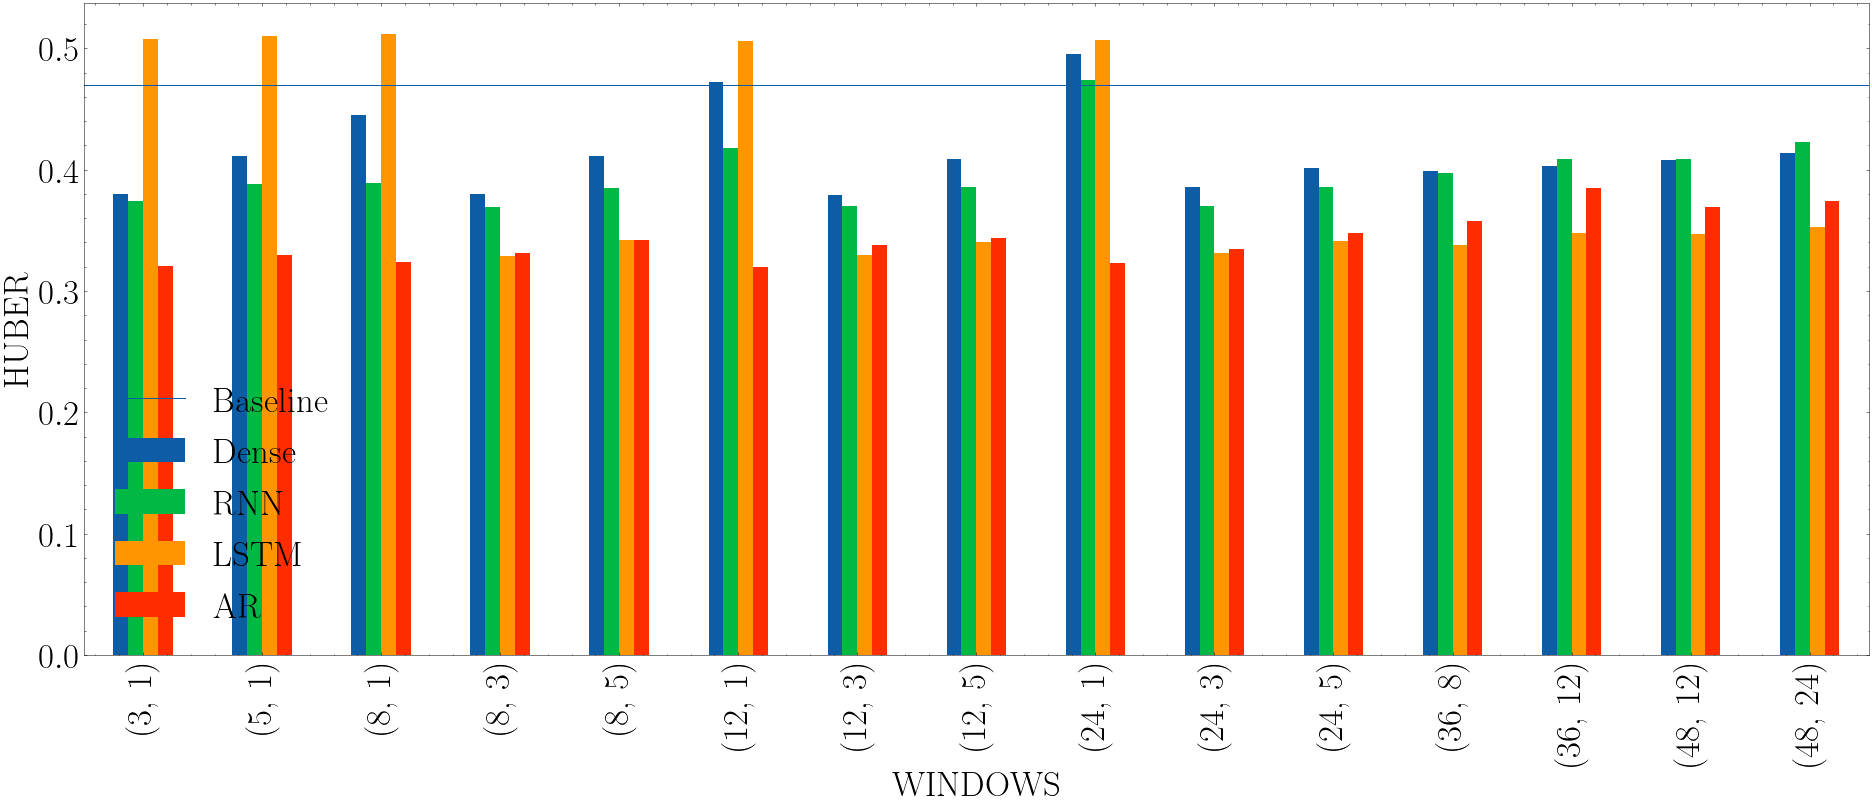
\includegraphics[width=15cm]{images/solution/metrics/HUBER.png}
    \caption{Resultados usando pérdida de Huber}
\end{figure}

\begin{figure}[H]
    \centering
    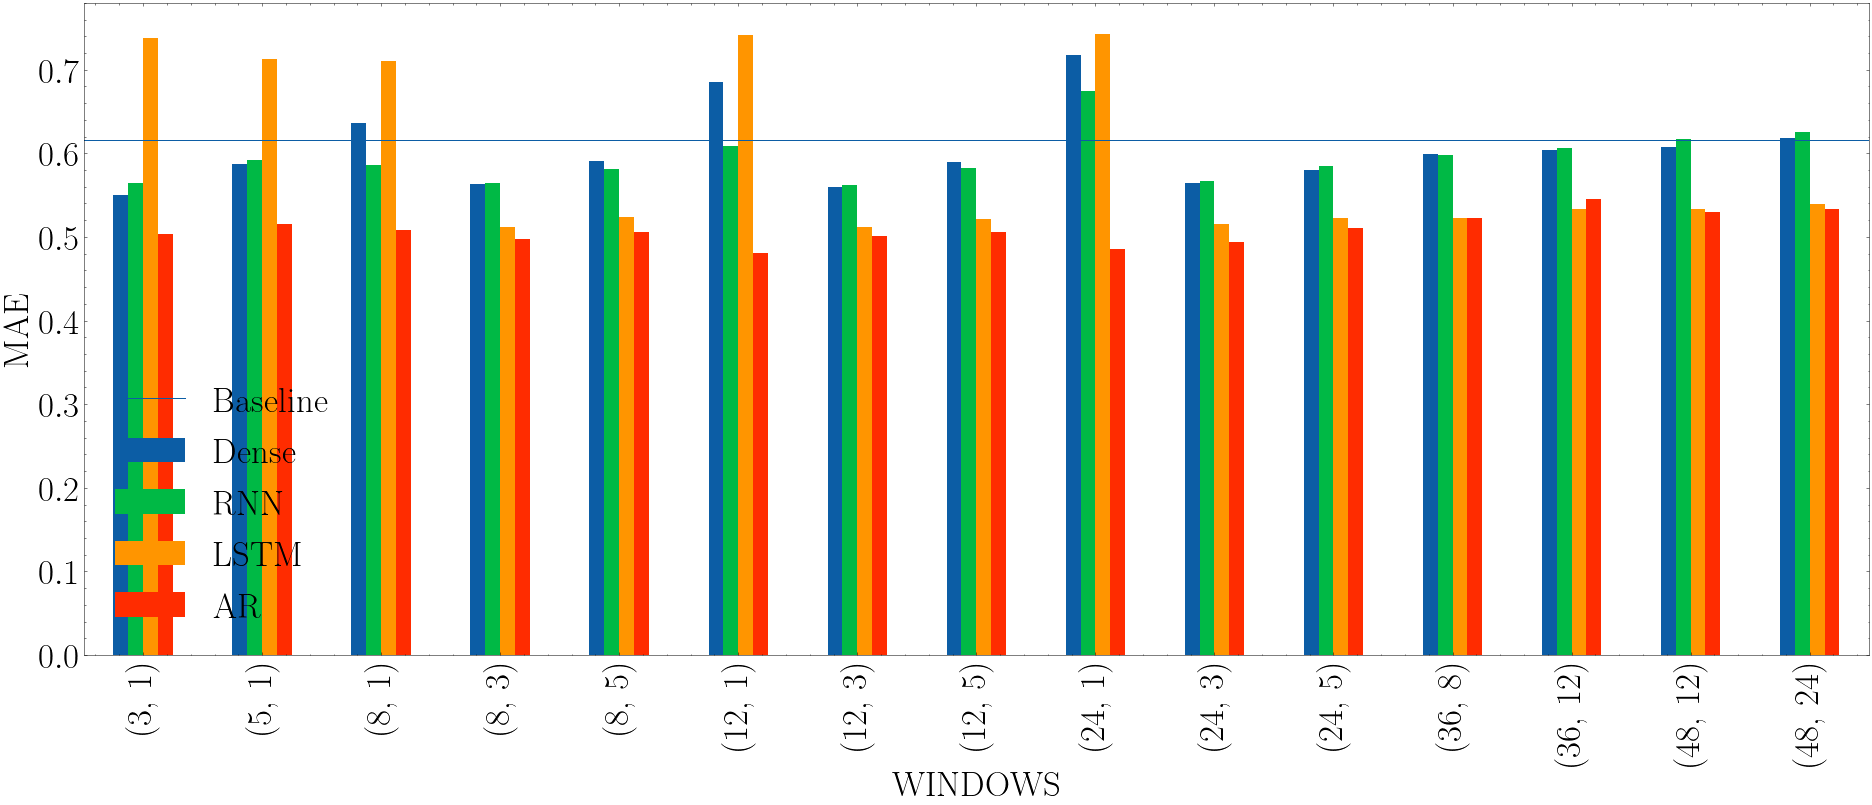
\includegraphics[width=15cm]{images/solution/metrics/MAE.png}
    \caption{Métricas usando MAE}
\end{figure}

\begin{figure}[H]
    \centering
    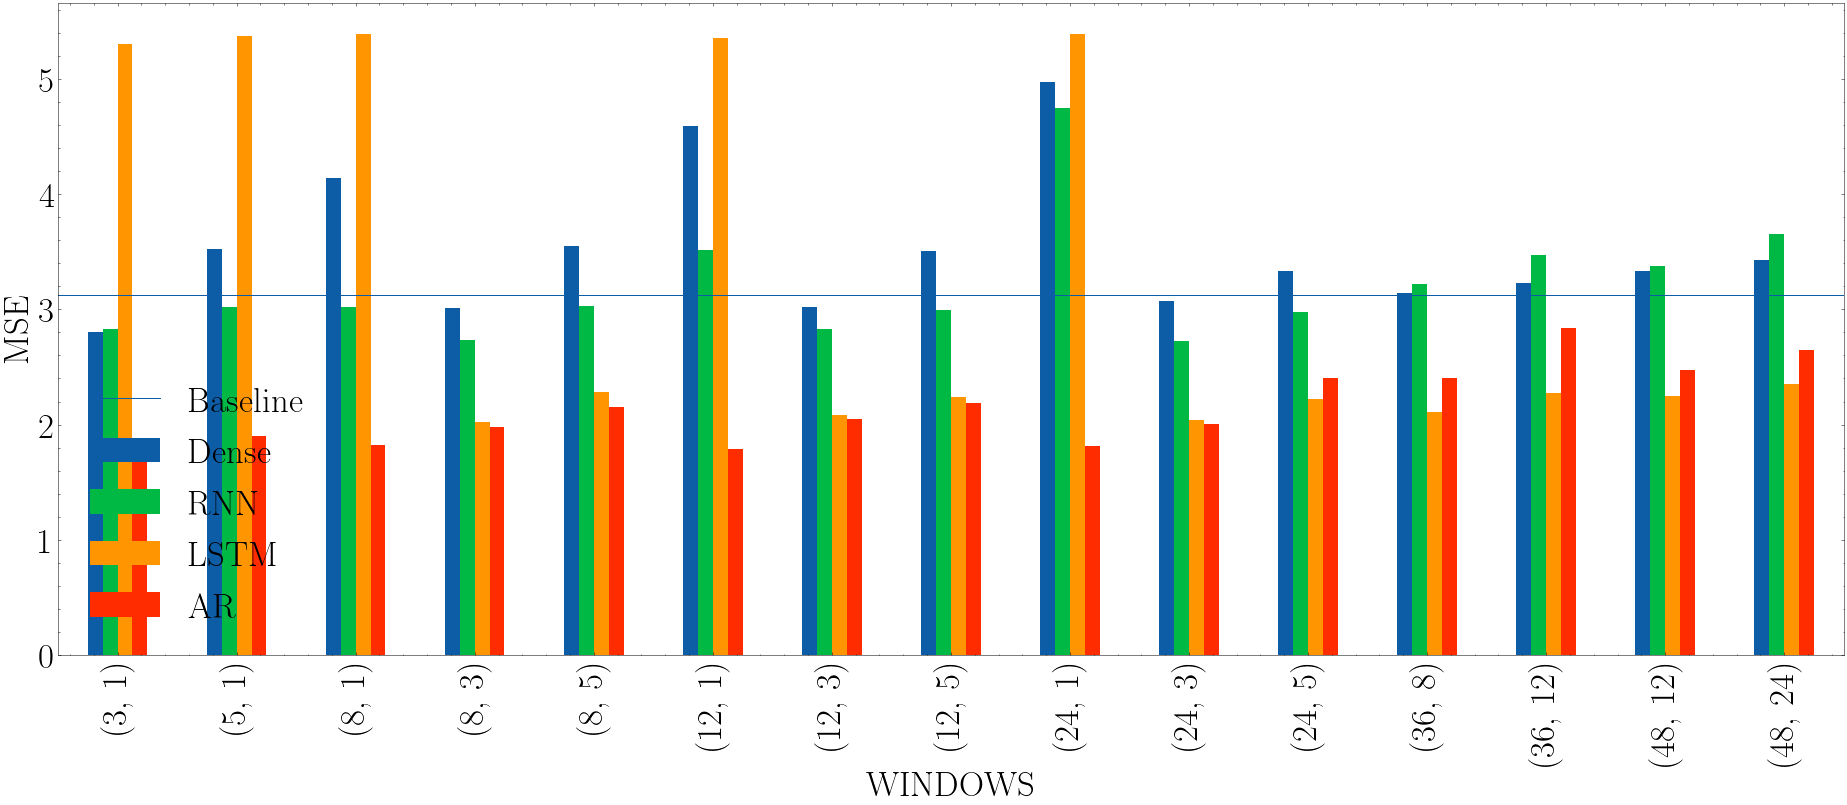
\includegraphics[width=15cm]{images/solution/metrics/MSE.png}
    \caption{Métricas usando MSE}
\end{figure}

\begin{figure}[H]
    \centering
    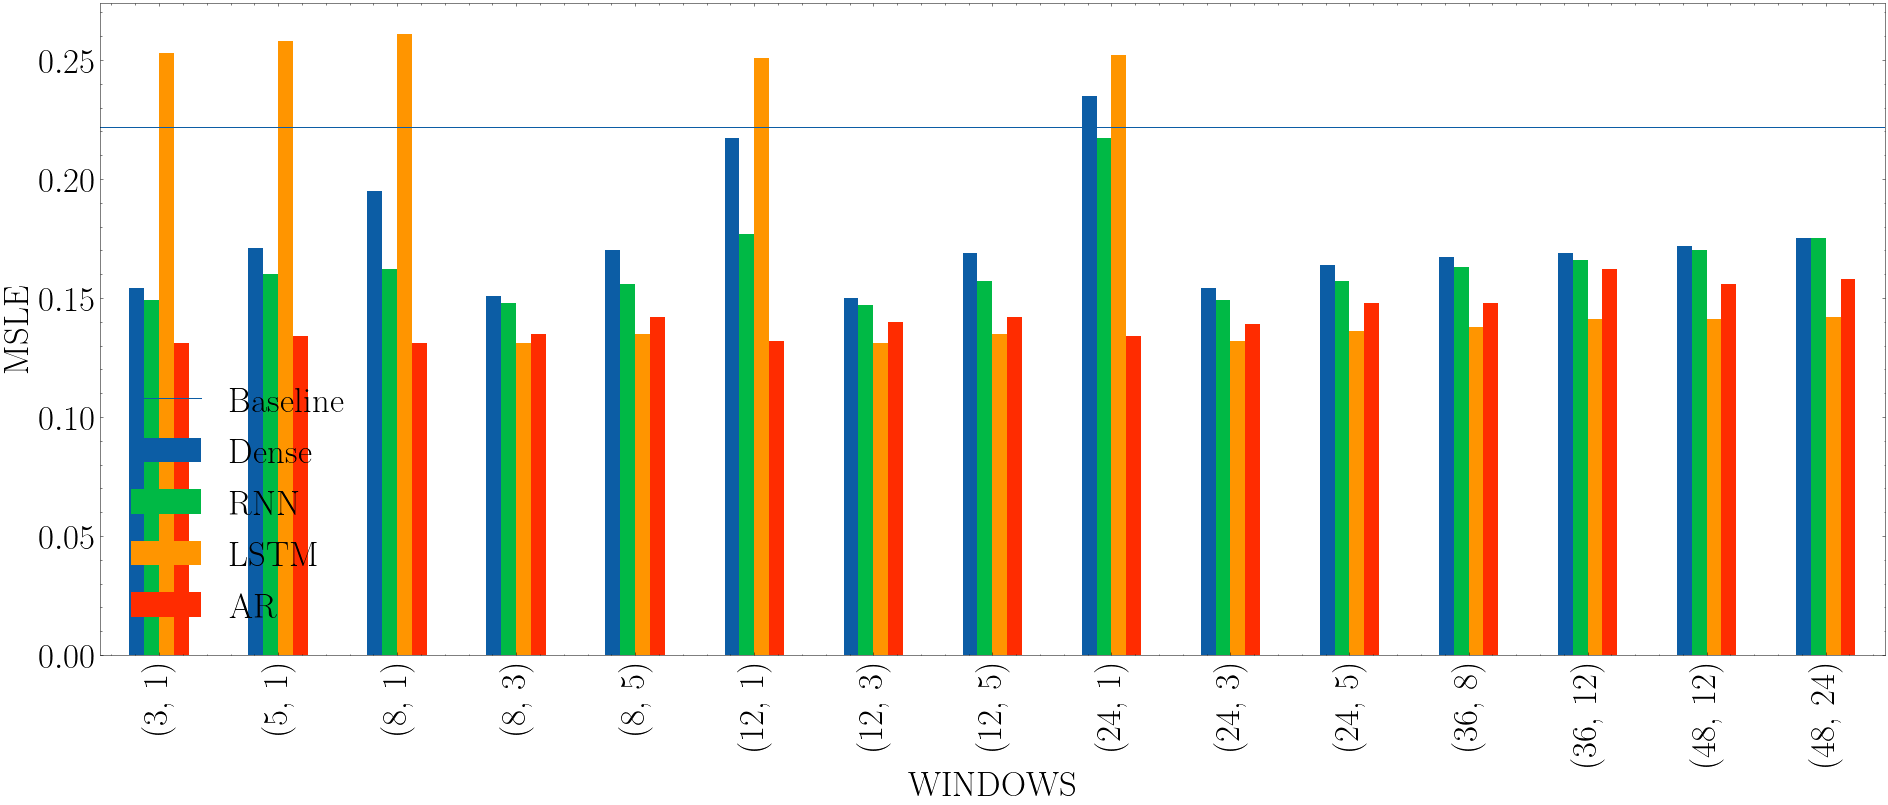
\includegraphics[width=15cm]{images/solution/metrics/MSLE.png}
    \caption{Métricas usando MSLE}
\end{figure}

\begin{figure}[H]
    \centering
    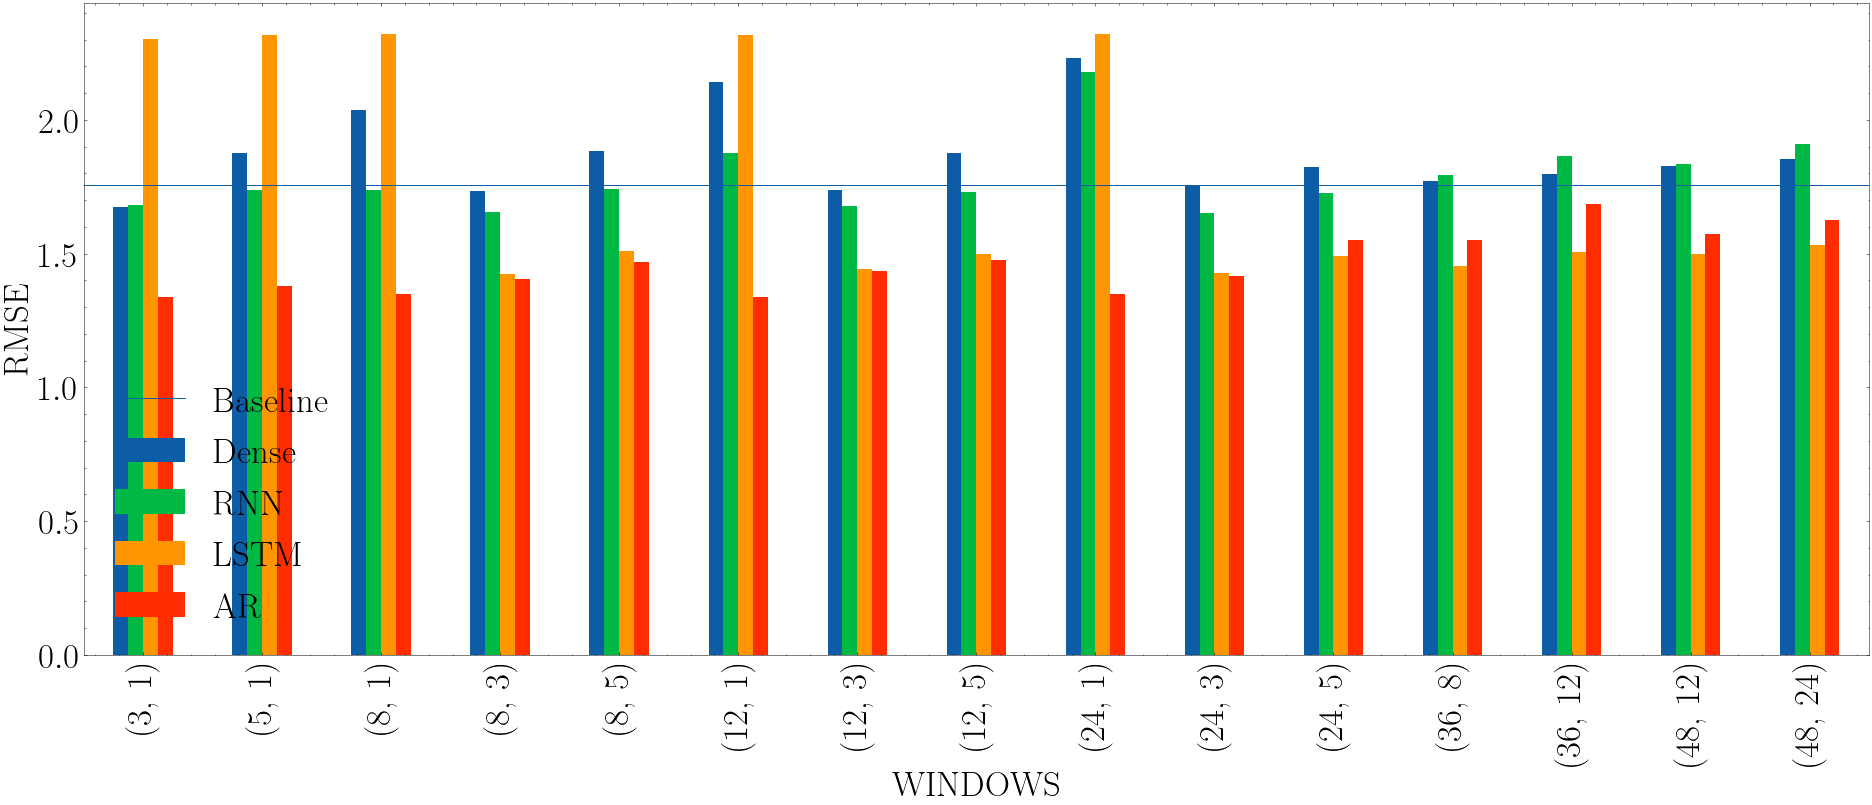
\includegraphics[width=15cm]{images/solution/metrics/RMSE.png}
    \caption{Métricas usando RMSE}
\end{figure}

\begin{figure}[H]
    \centering
\end{figure}

\newpage
\section{Problemas encontrados}

Durante el desarrollo de este trabajo no hemos encontrado con distintos problemas tanto a la hora de desarrollar las redes neuronales como al preprocesado necesario para poder crear el \textit{dataset}.

\subsection{Estructura del dataset}
Toda red neuronal tiene como requisito tener una arquitectura bien definida antes de poder ser creada. Entre otros parámetros, hay que definir tanto la entrada como la salida con la que el modelo trabajará. Al principio del desarrollo, al entrenar las primeras redes de prueba, obteníamos valores muy malos para lo que estábamos esperando. Todo ello era consecuencia de la mala definición que se había llevado a cabo para entrenar las redes.
\newline

Principalmente el error se encontraba en qué estaba contemplando desde el principio que una red pudiese aceptar una matriz como entrada, lo cual, no es cierta dicha afirmación. Una red siempre tiene que trabajar con vectores para las variables $x$ e $y$.
\newline

Posteriormente, desarrollé una estructura que tenía más sentido y con la cual la red obtenía mejores resultados. El problema de esta solución fue el tiempo de entrenamiento cuando se intentaba entrenar a una red básica. Era inviable seguir con esta estructura de datos.
\newline

Finalmente, tras varias reuniones con el tutor y con ayuda de un estudiante de doctorado llegamos a la conclusión que la mejor forma de entrenar a la red neuronal era con la estructura de datos que se ha explicado con anterioridad en este trabajo. Esta solución a pesar de ser muy intuitiva y fácil de entender, me ha costado una gran cantidad de tiempo llegar a ella.


\subsection{Desarrollo del preprocesado}
Para poder desarrollar una estructura de datos con que se puedan generar los modelos de las redes neuronales, es necesario previamente reestructurar el \textit{dataset} que usamos a un \textit{dataset} con el que se puedan generar las ventanas necesarias.
\newline

Para ello es necesario usar algún tipo de librería que facilite este proceso. En este trabajo se ha decidido usar \verb|DataFrame| de \textit{pandas} junto con otras librerías como \textit{numpy} o \textit{tensorflow}, las cuales eran mi primera vez usándolas pero que me he podido adaptar con facilidad.
\newline

A pesar de ello, me he encontrado con más problemas de los esperados a la hora de usar estas librerías y los cuales me han ralentizado el desarrollo. Además, muchas de las funciones que han sido desarrolladas no estaba seguro de si realizaban la tarea que se les encomendaba y por ello, he dedicado también parte de tiempo a escribir algunos test unitarios para asegúrame que el código era bueno.
\newline

Muchos de estos problemas tienen su origen a la hora de trabajar con más de 3 dimensiones. A partir de ese punto, es mucho más complejo para el cerebro humano poder tratar estructuras de este estilo y es importante realizar un estudio y un pseudocódigo de lo que se quiere hacer previamente. Esto sin duda alguna trataré de aplicarlo a proyectos futuros: dedicar más tiempo al diseño.

\subsection{Problema de \textit{overfitting}}

El problema del \textit{overfitting} es un problema común cuando se entrenan redes neuronales. Como se explica en la sección \ref{overfitting}, el \textit{overfitting} aparece tras un período de tiempo en el que la red ya ha aprendido y comienza a memorizar los datos, provocando que no se adapte a nuevas situaciones correctamente y pudiendo incluso emperorar los resultados del modelo.
\newline

Por esa razón, he dedicado parte de mi trabajo al estudio de como evitar el \textit{overfitting}. En un principio se usó la estrategia de trabajar con reguladores, que son ecuaciones con las cuales los pesos de una red se cambian con más lentitud. Pero esta solución, no ha tenido los resultados esperados. Lo que se conseguía con ello, era que el \textit{overfitting} aparecise pero en iteraciones del entrenamiento mucho más avanzadas, por lo que desestimé este el uso de regulizadores.
\newline

Finalmente, en los modelos actuales se han usado dos técnicas para evitar el \textit{overfitting}. En primer lugar, se ha usado una técnica por la cual se elige una tasa de aprendizaje con la cual el modelo converja a la hora del cálculo del gradiente. Esta técnica se basa en usar varios valores de la tasa de aprendizaje y estudiando como el descenso del gradiente se comporta respecto a ello. En segundo lugar, se ha usado la técnica del uso de \textit{Dropout} (ver sección \ref{dropout}), que básicamente activa y desactiva conexiones entre neuronas en la red de forma aleatoria para que ninguna sea prescindible, es decir, que contenga gran parte de conocimiento respecto a los patrones que se quieren predecir.

\newpage
\section{Conclusiones}

Con referencia al propio modelo de regresión y a los resultados obtenidos, se podría afirmar que la las siguientes conclusiones:
1. Las técnicas de aprendizaje de la máquina y específicamente el bosque aleatorio tienen un gran potencial en el campo de la ingeniería civil y el transporte. Si hay una gran cantidad de datos disponibles, los algoritmos de aprendizaje de la máquina pueden ser usados para hacer pronósticos muy precisos.

2. Incluso si se siente un poco contraintuitivo, para el modelo inicial (sólo bosque aleatorio) y el bosque aleatorio sin tendencia; predicción del recuento total utilizando dos modelos separados para usuarios ocasionales y registrados y sumándolos da una precisión muy similar a la de ...prediciéndolo con un solo modelo. Sin embargo, estos dos enfoques no son exactamente los lo mismo. El modelo que prevé por separado los usuarios registrados y los usuarios ocasionales puede utilizarse para entender mejor el comportamiento de cada tipo de usuario. Por otro lado, el modelo único es la mitad de lo que cuesta computacionalmente entrenar y optimizar. La elección entre estas dos opciones deben hacerse dependiendo del objetivo del modelo.

3. Un defecto importante del algoritmo de bosque aleatorio es su incapacidad para captar las tendencias que se muestran en los datos de capacitación si el conjunto de pruebas tiene valores más altos o más bajos para la variable que impulsa la tendencia que los del conjunto de trenes. Esto puede solucionarse desviando la tendencia si la tendencia puede observarse fácilmente o si se conoce previamente su causa, como se muestra en este proyecto. Esto se aplica a las tendencias monótonas crecientes o decrecientes en general, no sólo a las tendencias temporales.

4. Las variables meteorológicas adicionales construidas utilizando las existentes para tener en cuenta las fluctuaciones meteorológicas durante el día no ayudan a mejorar la precisión del modelo

Traducción realizada con la versión gratuita del traductor www.DeepL.com/Translator

Después de evaluar la exactitud del modelo a través de las conclusiones del modelo de regresión, el Se puede abordar la posible utilidad de esos resultados. Ambos conjuntos de conclusiones han sido separadas porque estas conclusiones son en cierto modo consecuencia de las primeras.
Los métodos de predicción y en particular los alimentados por datos e ingeniados con el aprendizaje de la máquina han demostrado ser una herramienta muy útil en el funcionamiento de un sistema de compartición de bicicletas.

Los modelos descritos en este proyecto requieren un poco de tiempo de ajuste para encontrar los parámetros óptimos, pero una vez que esos parámetros se optimizan, se pueden entrenar y desplegar rápidamente. La tendencia a la regresión lineal, en combinación con el modelo de bosque aleatorio, podría utilizarse para predecir la demanda de bicicletas así como la demanda de plazas de aparcamiento en cada estación (utilizando un modelo diferente para cada una de esas demandas). Esto permitiría al operador del sistema de bicicletas compartidas anticipar esas demandas utilizando un sistema de reposicionamiento dinámico, facilitando una de las principales causas de pérdida de clientes para los sistemas de bicicletas compartidas.

Además, estos modelos también podrían aplicarse a los sistemas de incentivos de equilibrio de bicicletas para diseñar el modelo de incentivos, combinando también las plazas de aparcamiento y las demandas de bicicletas para predecir qué las estaciones necesitarán más bicicletas y cuáles no. Además, las técnicas de aprendizaje de las máquinas podría desarrollarse para medir la eficacia del sistema de incentivos.

Este proyecto es un ejemplo excelente de la aplicación de las metodologías analíticas modernas a las problemas de ingeniería y transporte para generar valor mejorando la experiencia de los usuarios del sistema de transporte.



Cosas que he aprendido
Aprendido 

\newpage
\section{Trabajo futuro}\label{future_work}

Gran parte de este proyecto ha sido en el estudio teórico del concepto de las redes neuronales mientras que la aplicación práctica de lo aprendido ha sido la otra parte del tiempo dedicado. En esta parte práctica, principalmente, se ha invertido tiempo tanto en el aprendizaje de las librerías que se usan en la industria como pueden ser \textit{Tensorflow} y \textit{Pandas}, al igual que la dedicación en el entendimiento del problema y estudio de diferentes modelos y estudiar su comportamiento. Con este trabajo por lo tanto ha quedado demostrado que el mejor modelo que ha funcionado ha sido el auto-regresivo.
\newline

Como parte del trabajo futuro se propone mejorar este modelo para minimizar todo lo posible las métricas y proponer un modelo que obtenga resultados parecidos o mejores al estado del arte actual. Para ello, se podría estudiar más en profundidad tanto los parámetros de la red como la tasa de aprendizaje, el optimizador o el error. Pero, añadiendo más información al \textit{dataset} podría ser más útil, puesto que a mayor cantidad de datos, más preciso será el modelo. Se podrían usar por ejemplo variables como si es día festivo o la condiciones meteorológicas. Y esta es una de las principales diferencias que existen entre el \textit{dataset} usado en este proyecto y en otros. El \textit{dataset} usado solo contaba con tres variables sobre la información temporal: \textit{hour}, \textit{day\_of\_month} y \textit{month} y por lo tanto, no cabe duda que añadiendo estas cantidades de variables que aporten información sobre los patrones de alquiler de bicicletas, el modelo mejorase considerablemente.
\newline

Otro aspecto a mejorar de este proyecto sería la explotación de los resultados en algún tipo de herramienta útil a la empresa o a los usuarios. Los modelos entrenados simplemente han sido usados para computar las métricas y posteriormente han sido descartados puesto que no había planes de usarlos en producción. Por el contrario, si hubiese existido algún proyecto haciendo uso de los modelos, estos se podría haber guardado en un fichero y se podría usar en diferentes herramientas. Por ejemplo, una aplicación web que indique al usuario la predicción de bicicletas disponibles para cierta hora o un software que permite a los gestores de logística reubicar las bicicletas de forma más eficiente. Estas y otras aplicaciones podrían usar como módulo principal algún modelo de red neuronal explicado en este proyecto.
\newline





TODO EXLICAR QUE OPTIMIZADOR HA SIDO USADO


\newpage
\printbibliography[heading=bibnumbered] % Última sección, numerada, para la bibliografía
\newpage

\appendix


\section{Muestra del \textit{dataset} original de \textit{Divvy}}\label{app:original_dataset}

\begin{table}[H]
    \centering
    \tiny
    \rotatebox{90}{
   \begin{tabular}{lrllrlrlrlllr}
\toprule
          start\_time &             end\_time & tripduration &  from\_station\_id &                     from\_station\_name &  to\_station\_id &                       to\_station\_name &  gender &  birthyear \\
\midrule
 2019-09-23 16:48:09 &  2019-09-23 17:01:57 &        828.0 &               44 &                State St \& Randolph St &             21 &            Aberdeen St \& Jackson Blvd &     NaN &        NaN \\
 2019-08-19 18:18:41 &  2019-08-19 18:29:20 &        639.0 &              287 &               Franklin St \& Monroe St &            110 &                 Dearborn St \& Erie St &    Male &     1990.0 \\
 2019-01-08 08:42:22 &  2019-01-08 08:53:58 &        696.0 &               66 &                  Clinton St \& Lake St &            161 &                 Rush St \& Superior St &    Male &     1971.0 \\
 2019-05-18 13:27:52 &  2019-05-18 13:53:41 &      1,549.0 &               94 &               Clark St \& Armitage Ave &             35 &               Streeter Dr \& Grand Ave &    Male &     1988.0 \\
 2019-03-01 07:04:37 &  2019-03-01 07:12:09 &        452.0 &              174 &                 Canal St \& Madison St &             48 &            Larrabee St \& Kingsbury St &    Male &     1966.0 \\
 2019-03-13 18:13:48 &  2019-03-13 18:17:25 &        217.0 &              210 &             Ashland Ave \& Division St &            130 &               Damen Ave \& Division St &    Male &     1995.0 \\
 2019-08-11 20:05:13 &  2019-08-11 20:14:25 &        552.0 &               93 &             Sheffield Ave \& Willow St &            143 &             Sedgwick St \& Webster Ave &  Female &     1995.0 \\
 2019-01-24 16:50:10 &  2019-01-24 17:21:20 &      1,870.0 &              525 &              Glenwood Ave \& Touhy Ave &            243 &           Lincoln Ave \& Sunnyside Ave &  Female &     1986.0 \\
 2019-07-27 13:19:12 &  2019-07-27 13:33:34 &        862.0 &               72 &                  Wabash Ave \& 16th St &            197 &             Michigan Ave \& Madison St &    Male &     1995.0 \\
 2019-07-31 21:52:44 &  2019-07-31 22:22:41 &      1,796.0 &               52 &                Michigan Ave \& Lake St &             58 &          Marshfield Ave \& Cortland St &     NaN &        NaN \\
 2019-05-14 10:38:31 &  2019-05-14 10:44:45 &        374.0 &              236 &             Sedgwick St \& Schiller St &             48 &            Larrabee St \& Kingsbury St &    Male &     1986.0 \\
 2019-06-16 19:25:32 &  2019-06-16 19:40:59 &        927.0 &               85 &                 Michigan Ave \& Oak St &            224 &                Halsted St \& Willow St &    Male &     1988.0 \\
 2019-06-10 12:18:33 &  2019-06-10 12:24:33 &        360.0 &               38 &                    Clark St \& Lake St &            197 &             Michigan Ave \& Madison St &    Male &     1993.0 \\
 2019-12-12 09:55:38 &  2019-12-12 10:21:01 &      1,522.0 &              296 &                Broadway \& Belmont Ave &             69 &                Damen Ave \& Pierce Ave &     NaN &        NaN \\
 2019-09-09 09:07:44 &  2019-09-09 09:25:01 &      1,036.0 &               26 &              McClurg Ct \& Illinois St &            620 &  Orleans St \& Chestnut St (NEXT Apts) &  Female &     1992.0 \\
 2019-07-04 09:15:21 &  2019-07-04 10:26:40 &      4,279.0 &               99 &               Lake Shore Dr \& Ohio St &              6 &                        Dusable Harbor &  Female &     1992.0 \\
 2019-11-26 08:21:39 &  2019-11-26 08:34:49 &        790.0 &              376 &             Artesian Ave \& Hubbard St &            217 &        Elizabeth (May) St \& Fulton St &  Female &     1980.0 \\
 2019-07-22 08:09:05 &  2019-07-22 08:16:59 &        473.0 &              138 &            Clybourn Ave \& Division St &            133 &              Kingsbury St \& Kinzie St &    Male &     1984.0 \\
 2019-05-10 18:43:10 &  2019-05-10 18:51:40 &        510.0 &               99 &               Lake Shore Dr \& Ohio St &            180 &                 Ritchie Ct \& Banks St &     NaN &        NaN \\
 2019-04-05 09:38:21 &  2019-04-05 09:48:30 &        609.0 &               46 &                  Wells St \& Walton St &            287 &               Franklin St \& Monroe St &    Male &     1992.0 \\
 2019-07-22 16:50:47 &  2019-07-22 17:01:03 &        616.0 &               91 &          Clinton St \& Washington Blvd &             19 &        Throop (Loomis) St \& Taylor St &    Male &     1997.0 \\
 2019-06-03 21:09:36 &  2019-06-03 21:41:00 &      1,884.0 &              276 &            California Ave \& North Ave &            316 &             Damen Ave \& Sunnyside Ave &    Male &     1976.0 \\
 2019-08-01 19:20:36 &  2019-08-01 19:40:00 &      1,164.0 &              130 &               Damen Ave \& Division St &            124 &              Damen Ave \& Cullerton St &  Female &     1990.0 \\
 2019-07-17 16:24:52 &  2019-07-17 16:39:45 &        893.0 &              157 &        Lake Shore Dr \& Wellington Ave &            268 &            Lake Shore Dr \& North Blvd &    Male &     1997.0 \\
 2019-10-09 15:58:44 &  2019-10-09 16:09:00 &        616.0 &              129 &             Blue Island Ave \& 18th St &            281 &                 Western Ave \& 24th St &    Male &     1988.0 \\
 2019-04-08 11:34:37 &  2019-04-08 11:46:25 &        708.0 &               25 &             Michigan Ave \& Pearson St &            196 &       Cityfront Plaza Dr \& Pioneer Ct &    Male &     1965.0 \\
 2019-06-11 17:40:58 &  2019-06-11 18:13:44 &      1,966.0 &               43 &          Michigan Ave \& Washington St &            254 &       Pine Grove Ave \& Irving Park Rd &     NaN &        NaN \\
 2019-05-25 05:47:49 &  2019-05-25 06:04:43 &      1,014.0 &               66 &                  Clinton St \& Lake St &             97 &                          Field Museum &    Male &     1976.0 \\
 2019-08-18 11:29:24 &  2019-08-18 11:51:34 &      1,330.0 &              199 &                Wabash Ave \& Grand Ave &            161 &                 Rush St \& Superior St &  Female &     1964.0 \\
 2019-09-10 08:31:13 &  2019-09-10 08:37:56 &        403.0 &               85 &                 Michigan Ave \& Oak St &            194 &                Wabash Ave \& Wacker Pl &    Male &     1993.0 \\
 2019-10-25 15:59:12 &  2019-10-25 16:07:03 &        471.0 &              211 &                St. Clair St \& Erie St &            636 &               Orleans St \& Hubbard St &  Female &     1981.0 \\
 2019-08-13 16:01:17 &  2019-08-13 16:05:56 &        279.0 &              121 &       Blackstone Ave \& Hyde Park Blvd &            418 &                   Ellis Ave \& 53rd St &    Male &     1966.0 \\
 2019-07-08 20:05:44 &  2019-07-08 20:13:38 &        473.0 &              156 &             Clark St \& Wellington Ave &            131 &             Lincoln Ave \& Belmont Ave &    Male &     1984.0 \\
 2019-08-11 13:15:22 &  2019-08-11 13:18:36 &        194.0 &               94 &               Clark St \& Armitage Ave &            289 &                 Wells St \& Concord Ln &    Male &     1990.0 \\
 2019-03-12 13:50:21 &  2019-03-12 13:54:03 &        222.0 &               32 &            Racine Ave \& Congress Pkwy &             22 &                    May St \& Taylor St &    Male &     1993.0 \\
 2019-12-07 08:29:06 &  2019-12-07 08:46:15 &      1,028.0 &              141 &                Clark St \& Lincoln Ave &            347 &                Ashland Ave \& Grace St &    Male &     1991.0 \\
 2019-10-03 18:58:44 &  2019-10-03 19:22:45 &      1,440.0 &              365 &          Halsted St \& North Branch St &            117 &              Wilton Ave \& Belmont Ave &    Male &     1987.0 \\
 2019-12-29 10:48:05 &  2019-12-29 10:58:48 &        642.0 &              299 &                Halsted St \& Roscoe St &            220 &                Clark St \& Drummond Pl &    Male &     1983.0 \\
 2019-07-07 00:04:09 &  2019-07-07 00:24:27 &      1,218.0 &              291 &              Wells St \& Evergreen Ave &              7 &           Field Blvd \& South Water St &    Male &     1989.0 \\
 2019-11-06 08:27:59 &  2019-11-06 08:33:24 &        325.0 &              190 &        Southport Ave \& Wrightwood Ave &             67 &         Sheffield Ave \& Fullerton Ave &  Female &     1993.0 \\
 2019-04-13 19:10:09 &  2019-04-13 19:16:08 &        359.0 &              627 &             LaSalle Dr \& Huron St (*) &             23 &               Orleans St \& Elm St (*) &  Female &     1976.0 \\
 2019-09-11 07:52:42 &  2019-09-11 08:05:43 &        781.0 &              331 &             Halsted St \& Clybourn Ave &             48 &            Larrabee St \& Kingsbury St &    Male &     1979.0 \\
 2019-07-10 18:28:05 &  2019-07-10 18:57:29 &      1,764.0 &              268 &            Lake Shore Dr \& North Blvd &             29 &              Noble St \& Milwaukee Ave &    Male &     1996.0 \\
 2019-08-09 10:48:54 &  2019-08-09 12:06:15 &      4,640.0 &              623 &                 Michigan Ave \& 8th St &            268 &            Lake Shore Dr \& North Blvd &     NaN &        NaN \\
 2019-08-08 05:39:47 &  2019-08-08 05:45:06 &        319.0 &              283 &             LaSalle St \& Jackson Blvd &             47 &                  State St \& Kinzie St &    Male &     1975.0 \\
 2019-06-07 17:48:11 &  2019-06-07 18:04:44 &        993.0 &              144 &             Larrabee St \& Webster Ave &            230 &               Lincoln Ave \& Roscoe St &    Male &     1989.0 \\
 2019-07-30 07:51:29 &  2019-07-30 08:06:40 &        910.0 &               13 &            Wilton Ave \& Diversey Pkwy &            359 &             Larrabee St \& Division St &  Female &     1991.0 \\
 2019-11-29 14:14:22 &  2019-12-03 20:45:36 &    369,074.0 &              343 &           Racine Ave \& Wrightwood Ave &             67 &         Sheffield Ave \& Fullerton Ave &  Female &     1960.0 \\
 2019-11-22 09:42:12 &  2019-11-22 10:16:53 &      2,080.0 &              131 &             Lincoln Ave \& Belmont Ave &            283 &             LaSalle St \& Jackson Blvd &    Male &     1976.0 \\
 2019-07-25 16:56:04 &  2019-07-25 16:58:51 &        166.0 &               36 &            Franklin St \& Jackson Blvd &             68 &                Clinton St \& Tilden St &    Male &     1968.0 \\
 2019-04-13 09:13:59 &  2019-04-13 09:16:34 &        155.0 &              229 &             Southport Ave \& Roscoe St &            227 &          Southport Ave \& Waveland Ave &  Female &     1984.0 \\
 2019-08-25 11:03:24 &  2019-08-25 11:37:46 &      2,062.0 &               90 &                       Millennium Park &             35 &               Streeter Dr \& Grand Ave &     NaN &        NaN \\
 2019-04-05 16:46:32 &  2019-04-05 17:00:32 &        840.0 &               68 &                Clinton St \& Tilden St &            138 &            Clybourn Ave \& Division St &    Male &     1990.0 \\
 2019-11-24 20:03:18 &  2019-11-24 20:08:39 &        320.0 &              419 &               Lake Park Ave \& 53rd St &            322 &                 Kimbark Ave \& 53rd St &    Male &     1995.0 \\
 2019-06-20 18:16:05 &  2019-06-20 18:23:50 &        465.0 &              287 &               Franklin St \& Monroe St &             90 &                       Millennium Park &    Male &     1981.0 \\
 2019-06-14 16:29:10 &  2019-06-14 16:40:44 &        694.0 &              182 &                     Wells St \& Elm St &            329 &         Lake Shore Dr \& Diversey Pkwy &    Male &     1992.0 \\
 2019-04-26 14:36:59 &  2019-04-26 15:31:05 &      3,246.0 &              577 &  Stony Island Ave \& South Chicago Ave &             11 &                Jeffery Blvd \& 71st St &  Female &     1992.0 \\
 2019-06-10 17:36:08 &  2019-06-10 17:50:58 &        890.0 &              283 &             LaSalle St \& Jackson Blvd &            182 &                     Wells St \& Elm St &    Male &     1996.0 \\
 2019-08-18 14:41:50 &  2019-08-18 14:51:00 &        549.0 &              330 &              Lincoln Ave \& Addison St &            166 &          Ashland Ave \& Wrightwood Ave &    Male &     1988.0 \\
 2019-05-03 06:07:25 &  2019-05-03 06:16:04 &        519.0 &               23 &               Orleans St \& Elm St (*) &            164 &                 Franklin St \& Lake St &    Male &     1977.0 \\
\bottomrule

\tablefootnote{Se omiten las columnas: \textit{bikeid}, \textit{tripid} y \textit{usertype}}
\end{tabular}}

\caption{Muestras aleatorias del \textit{dataset} original de Divvy}
\end{table}
\section{Muestra del \textit{dataset} de intervalos}\label{app:intervals_dataset}

\begin{table}[H]
    \centering
    \tiny
    \rotatebox{90}{
\begin{tabular}{lrrrrrrrrr}
\toprule
{} &  hour &  day\_of\_week &  month &  quantity\_1 &  quantity\_2 &  quantity\_3 &  quantity\_4 &  quantity\_631 &  quantity\_632 \\
start\_time          &       &              &        &             &             &             &             &               &               \\
\midrule
2019-09-22 03:00:00 &     3 &            5 &      9 &         0.0 &         0.0 &         0.0 &         0.0 &           0.0 &           0.0 \\
2017-01-10 00:00:00 &     0 &            2 &      1 &         0.0 &         0.0 &         1.0 &         0.0 &           0.0 &           0.0 \\
2019-12-01 01:00:00 &     1 &            5 &     12 &         1.0 &         0.0 &         0.0 &         0.0 &           0.0 &           0.0 \\
2018-01-02 17:00:00 &    17 &            1 &      1 &         0.0 &         0.0 &         0.0 &         0.0 &           0.0 &           0.0 \\
2018-11-01 14:00:00 &    14 &            3 &     11 &         0.0 &         0.0 &         4.0 &         1.0 &           0.0 &           0.0 \\
2017-01-23 03:00:00 &     3 &            1 &      1 &         0.0 &         0.0 &         0.0 &         0.0 &           1.0 &           0.0 \\
2018-11-12 16:00:00 &    16 &            7 &     11 &         0.0 &         0.0 &         0.0 &         0.0 &           0.0 &           1.0 \\
2019-12-25 12:00:00 &    12 &            1 &     12 &         0.0 &         0.0 &         0.0 &         0.0 &           0.0 &           0.0 \\
2019-02-01 00:00:00 &     0 &            3 &      2 &         0.0 &         0.0 &         0.0 &         0.0 &           0.0 &           0.0 \\
2017-03-04 08:00:00 &     8 &            6 &      3 &         0.0 &         0.0 &         0.0 &         1.0 &           0.0 &           0.0 \\
2018-03-25 20:00:00 &    20 &            6 &      3 &         1.0 &         0.0 &         0.0 &         0.0 &           1.0 &           2.0 \\
2019-06-08 07:00:00 &     7 &            4 &      6 &         3.0 &         4.0 &         0.0 &         4.0 &           0.0 &           0.0 \\
2017-09-30 19:00:00 &    19 &            6 &      9 &         2.0 &         8.0 &         2.0 &         1.0 &           2.0 &           0.0 \\
2018-08-22 21:00:00 &    21 &            2 &      8 &         0.0 &         0.0 &         2.0 &         1.0 &           3.0 &           0.0 \\
2017-02-22 08:00:00 &     8 &            3 &      2 &         0.0 &         0.0 &         0.0 &         0.0 &           0.0 &           1.0 \\
2017-07-05 18:00:00 &    18 &            3 &      7 &         1.0 &         3.0 &        17.0 &        10.0 &           1.0 &           3.0 \\
2019-07-21 11:00:00 &    11 &            5 &      7 &         0.0 &         1.0 &         5.0 &         5.0 &           0.0 &           0.0 \\
2019-07-27 00:00:00 &     0 &            4 &      7 &         1.0 &         0.0 &         0.0 &         0.0 &           0.0 &           0.0 \\
2018-12-09 21:00:00 &    21 &            6 &     12 &         0.0 &         0.0 &         0.0 &         0.0 &           0.0 &           0.0 \\
2018-04-16 06:00:00 &     6 &            7 &      4 &         1.0 &         0.0 &         0.0 &         0.0 &           0.0 &           0.0 \\
2019-02-27 13:00:00 &    13 &            1 &      2 &         0.0 &         1.0 &         3.0 &         0.0 &           0.0 &           0.0 \\
2019-10-25 02:00:00 &     2 &            3 &     10 &         0.0 &         0.0 &         0.0 &         0.0 &           0.0 &           0.0 \\
2017-12-26 18:00:00 &    18 &            2 &     12 &         0.0 &         0.0 &         0.0 &         0.0 &           0.0 &           0.0 \\
2017-10-29 07:00:00 &     7 &            7 &     10 &         2.0 &         0.0 &         0.0 &         0.0 &           0.0 &           1.0 \\
2018-01-20 11:00:00 &    11 &            5 &      1 &         0.0 &         0.0 &         1.0 &         1.0 &           2.0 &           0.0 \\
2018-06-08 03:00:00 &     3 &            4 &      6 &         0.0 &         0.0 &         0.0 &         0.0 &           0.0 &           0.0 \\
2019-10-29 06:00:00 &     6 &            7 &     10 &         0.0 &         0.0 &         0.0 &         0.0 &           0.0 &           0.0 \\
2019-11-25 11:00:00 &    11 &            6 &     11 &         3.0 &         0.0 &         2.0 &         8.0 &           0.0 &           0.0 \\
2017-06-06 09:00:00 &     9 &            2 &      6 &         1.0 &         3.0 &         1.0 &        10.0 &           2.0 &           2.0 \\
2018-03-16 22:00:00 &    22 &            4 &      3 &         0.0 &         3.0 &         0.0 &         0.0 &           0.0 &           0.0 \\
2019-11-06 10:00:00 &    10 &            1 &     11 &         0.0 &         4.0 &         0.0 &         0.0 &           0.0 &           0.0 \\
2017-06-11 17:00:00 &    17 &            7 &      6 &         1.0 &        11.0 &        21.0 &        10.0 &           4.0 &           3.0 \\
2018-07-21 18:00:00 &    18 &            5 &      7 &         0.0 &         0.0 &         3.0 &         2.0 &           0.0 &           0.0 \\
2019-05-25 11:00:00 &    11 &            4 &      5 &         0.0 &         0.0 &         6.0 &         0.0 &           1.0 &           1.0 \\
2018-03-02 01:00:00 &     1 &            4 &      3 &         5.0 &         0.0 &         0.0 &         0.0 &           0.0 &           0.0 \\
2018-12-21 06:00:00 &     6 &            4 &     12 &         0.0 &         0.0 &         0.0 &         0.0 &           0.0 &           0.0 \\
2019-01-07 06:00:00 &     6 &            6 &      1 &         0.0 &         0.0 &         0.0 &         0.0 &           0.0 &           0.0 \\
2018-05-04 13:00:00 &    13 &            4 &      5 &         1.0 &         0.0 &         5.0 &         2.0 &           3.0 &           3.0 \\
2019-01-25 09:00:00 &     9 &            3 &      1 &         0.0 &         0.0 &         0.0 &         0.0 &           0.0 &           0.0 \\
2019-11-24 19:00:00 &    19 &            5 &     11 &         0.0 &         0.0 &         0.0 &         0.0 &           0.0 &           0.0 \\
2018-10-18 16:00:00 &    16 &            3 &     10 &         1.0 &         2.0 &        14.0 &         5.0 &           0.0 &           0.0 \\
2018-07-14 23:00:00 &    23 &            5 &      7 &         1.0 &         1.0 &         6.0 &         0.0 &           0.0 &           0.0 \\
2017-08-10 02:00:00 &     2 &            4 &      8 &         0.0 &         0.0 &         0.0 &         0.0 &           0.0 &           1.0 \\
2017-04-13 00:00:00 &     0 &            4 &      4 &         0.0 &         0.0 &         0.0 &         0.0 &           3.0 &           0.0 \\
2017-03-23 20:00:00 &    20 &            4 &      3 &         0.0 &         0.0 &         0.0 &         0.0 &           0.0 &           0.0 \\
2018-09-04 16:00:00 &    16 &            1 &      9 &         3.0 &        21.0 &        20.0 &        10.0 &           2.0 &           2.0 \\
2019-04-11 09:00:00 &     9 &            2 &      4 &         0.0 &         0.0 &         0.0 &         1.0 &           0.0 &           0.0 \\
2019-05-25 01:00:00 &     1 &            4 &      5 &         0.0 &         0.0 &         0.0 &         0.0 &           0.0 &           0.0 \\
2018-01-03 11:00:00 &    11 &            2 &      1 &         0.0 &         1.0 &         1.0 &         0.0 &           4.0 &           0.0 \\
2018-04-19 00:00:00 &     0 &            3 &      4 &         4.0 &         0.0 &         0.0 &         0.0 &           0.0 &           0.0 \\
2019-09-27 16:00:00 &    16 &            3 &      9 &         0.0 &         6.0 &        14.0 &         7.0 &           0.0 &           2.0 \\
2017-02-16 01:00:00 &     1 &            4 &      2 &         0.0 &         0.0 &         0.0 &         0.0 &           0.0 &           0.0 \\
2017-05-09 19:00:00 &    19 &            2 &      5 &         0.0 &         2.0 &         1.0 &         3.0 &           0.0 &           1.0 \\
2019-11-26 01:00:00 &     1 &            7 &     11 &         1.0 &         0.0 &         0.0 &         0.0 &           1.0 &           0.0 \\
2018-08-12 05:00:00 &     5 &            6 &      8 &         0.0 &         0.0 &         0.0 &         0.0 &           0.0 &           0.0 \\
\bottomrule
\tablefootnote{Se omiten las todas las estaciones cuyo \textit{id} sea entre $5$ y $631$}

\end{tabular}}

\caption{Muestras aleatorias del \textit{dataset} dividido por intervalos}
\end{table}
% \newpage
\clearpage
\printglossary[type=\acronymtype]
% \printglossary

\newpage


\end{document}